\documentclass[9pt,table,xcolor=dvipsnames]{beamer}% {{{
\setbeamercovered{invisible}
% \includeonlyframes{current}
 %  \documentclass[compress,trans,9pt,table]{beamer}
% \documentclass[compress,9pt,usenames,dvipsnames]{beamer}
% \documentclass[9pt]{beamer}
% \usepackage[utf8]{inputenc}
\setbeamercovered{dynamic}
\usepackage{etex}
\usepackage{amsmath}
\usepackage{graphicx,url,psfrag}
\usepackage{tikz}
\usetikzlibrary{
  arrows,
  arrows.meta,
  calc,
  decorations.fractals,
  decorations.pathreplacing,
  graphs,
  mindmap,
  positioning,
  shapes.geometric,
  through,shapes,patterns,
  trees,
  }
\usepackage{smartdiagram}
\usesmartdiagramlibrary{additions}
\usepackage[center]{subfigure}
\usepackage{enumerate}
\usepackage[makeroom]{cancel}
\usepackage{mathtools}
\newcommand{\Crossme}[1]{\!\!
\tikz [black,x=1.1em,y=1.1em,line width=.4ex]
\draw (-0.5,-0.5) -- (0,0) node {\footnotesize #1} -- (0.5,0.5) (0.5,-0.5) -- (-0.5,0.5);}%
\newcommand{\Checkme}[1]{\!\!
\tikz [x=1.1em,y=1.1em,line width=.4ex]
\draw [black] (0,0.7) -- (0.3,0) --(0.9,1.0) (0.5,0.5) node {\footnotesize #1};}
\beamerdefaultoverlayspecification{<+-| alert@+>} %(this will show line by line)
\beamerdefaultoverlayspecification{<+->} %(this will show line by
\usepackage{arydshln}
% Smiley face\Smiley{} \Frowny{}
\usepackage{marvosym}

% -------------------------------------------------
%  Set directory for figs
% -------------------------------------------------
\usepackage{grffile}
\graphicspath{{../2016-11-29-McGill/figs/}}

% -------------------------------------------------
%  Define colors
% -------------------------------------------------
% Darkmode
\usepackage{dbt}
\def\refcolor{cyan}
\newcommand{\myref}[1]{\small {\em #1}}
% \def\excolor{brown}
\usepackage{color}
\usepackage{xcolor}

\usepackage{makecell}
\usepackage{tabstackengine}
\renewcommand\theadalign{bc}
\renewcommand\theadfont{\bfseries}
\renewcommand\theadgape{\Gape[4pt]}
\renewcommand\cellgape{\Gape[4pt]}


% -------------------------------------------------
%  Define short-hand symbols.
% -------------------------------------------------
\newcommand{\B}{\textbf{B}}
\newcommand{\E}{\mathbb{E}}
\newcommand{\D}{\mathbb{D}}
\newcommand{\W}{\dot{W}}
\newcommand{\ud}{\ensuremath{\mathrm{d} }}
\newcommand{\Ceil}[1]{\left\lceil #1 \right\rceil}
\newcommand{\Floor}[1]{\left\lfloor #1 \right\rfloor}
\newcommand{\sgn}{\text{sgn}}
\newcommand{\Lad}{\text{L}_{\text{ad}}^2}
\newcommand{\SI}[1]{\mathcal{I}\left[#1 \right]}
\newcommand{\SIB}[2]{\mathcal{I}_{#2}\left[#1 \right]}
\newcommand{\Indt}[1]{1_{\left\{#1 \right\} }}
\newcommand{\LadInPrd}[1]{\left\langle #1 \right\rangle_{\text{L}_\text{ad}^2}}
\newcommand{\LadNorm}[1]{\left|\left|  #1 \right|\right|_{\text{L}_\text{ad}^2}}
\newcommand{\Norm}[1]{\left|\left|  #1   \right|\right|}
\newcommand{\Ito}{It\^{o} }
\newcommand{\Itos}{It\^{o}'s }
\newcommand{\spt}[1]{\text{supp}\left(#1\right)}
\newcommand{\InPrd}[1]{\left\langle #1 \right\rangle}
\newcommand{\mr}{\textbf{r}}
\newcommand{\Ei}{\text{Ei}}
\newcommand{\arctanh}{\operatorname{arctanh}}
\newcommand{\ind}[1]{\mathbb{I}_{\left\{ {#1} \right\} }}


\DeclareMathOperator{\esssup}{\ensuremath{ess\,sup}}

\newcommand{\steps}[1]{\vskip 0.3cm \textbf{#1}}
\newcommand{\calB}{\mathcal{B}}
\newcommand{\calC}{\mathcal{C}}
\newcommand{\calD}{\mathcal{D}}
\newcommand{\calE}{\mathcal{E}}
\newcommand{\calF}{\mathcal{F}}
\newcommand{\calG}{\mathcal{G}}
\newcommand{\calK}{\mathcal{K}}
\newcommand{\calH}{\mathcal{H}}
\newcommand{\calI}{\mathcal{I}}
\newcommand{\calL}{\mathcal{L}}
\newcommand{\calM}{\mathcal{M}}
\newcommand{\calN}{\mathcal{N}}
\newcommand{\calO}{\mathcal{O}}
\newcommand{\calT}{\mathcal{T}}
\newcommand{\calP}{\mathcal{P}}
\newcommand{\calR}{\mathcal{R}}
\newcommand{\calS}{\mathcal{S}}
\newcommand{\calV}{\mathcal{V}}
\newcommand{\bbC}{\mathbb{C}}
\newcommand{\bbF}{\mathbb{F}}
\newcommand{\bbN}{\mathbb{N}}
\newcommand{\bbP}{\mathbb{P}}
\newcommand{\bbZ}{\mathbb{Z}}
\newcommand{\myVec}[1]{\overrightarrow{#1}}
\newcommand{\sincos}{\begin{array}{c} \cos \\ \sin \end{array}\!\!}
\newcommand{\CvBc}[1]{\left\{\:#1\:\right\}}
\newcommand*{\one}{{ {\rm 1\mkern-1.5mu}\!{\rm I} }}
\newcommand{\Lip}{\text{Lip}}

\newcommand{\bH}{\ensuremath{\mathrm{H} }}
\newcommand{\Ai}{\ensuremath{\mathrm{Ai} }}

\newcommand{\R}{\mathbb{R}}
\newcommand{\myEnd}{\hfill$\square$}
\newcommand{\ds}{\displaystyle}
\newcommand{\Shi}{\text{Shi}}
\newcommand{\Chi}{\text{Chi}}
\newcommand{\Erf}{\ensuremath{\mathrm{erf} }}
\newcommand{\Erfc}{\ensuremath{\mathrm{erfc} }}
\newcommand{\He}{\ensuremath{\mathrm{He} }}
\newcommand{\Res}{\ensuremath{\mathrm{Res} }}

\newcommand{\mySeparateLine}{\begin{center}
 \makebox[\linewidth]{\rule{0.6\paperwidth}{0.4pt}}
\end{center}}

% The following is to increase the gap in underbrace.
% Followed by https://tex.stackexchange.com/questions/13843/vertical-spacing-with-underbrace-command/13864
\newcommand*\mystrut[1]{\vrule width0pt height0pt depth#1\relax}

% % % Define danger sign
\newcommand*{\TakeFourierOrnament}[1]{{%
\fontencoding{U}\fontfamily{futs}\selectfont\char#1}}
\newcommand*{\danger}{\TakeFourierOrnament{66}}

\theoremstyle{definition}
% \newtheorem{definition}[theorem]{Definition}
% \newtheorem{hypothesis}[theorem]{Hypothesis}
\newtheorem{assumption}[theorem]{Assumption}

\theoremstyle{plain}
% \newtheorem{theorem}{Theorem}
% \newtheorem{corollary}[theorem]{Corollary}
% \newtheorem{lemma}[theorem]{Lemma}
\newtheorem{proposition}[theorem]{Proposition}

\mode<presentation>
{
%      \usetheme{Warsaw}
%     \usetheme{JuanLesPins}
%  \usetheme{Hannover}
%  \usetheme{Montpellier}
   % \useoutertheme{default}
  % or ...

  \setbeamercovered{transparent}
  % or whatever (possibly just delete it)
 \setbeamertemplate{frametitle}{
  \begin{centering}
    \color{lgtblue!70!black}{\insertframetitle}
    \par
  \end{centering}
  }
}
\usefoottemplate{\hfill \insertframenumber{} / 34}
% \inserttotalframenumber

\usepackage[english]{babel}
% or whatever

% \usepackage[latin1]{inputenc}
% or whatever

\usepackage{times}
\usepackage[T1]{fontenc}
% Or whatever. Note that the encoding and the font should match. If T1
% does not look nice, try deleting the line with the fontenc.

% \DeclareMathOperator{\Lip}{Lip}
\DeclareMathOperator{\lip}{l}
% \DeclareMathOperator{\Vip}{\overline{v}}
% \DeclareMathOperator{\vip}{\underline{v}}
% \DeclareMathOperator{\vv}{v}
% \DeclareMathOperator{\BC}{BC}
% \DeclareMathOperator{\CH}{CD}

\usepackage{pgfpages}
% \setbeameroption{show notes}
% \setbeamertemplate{note page}[plain]
% \setbeameroption{second mode text on second screen=right}
% \setbeameroption{show notes on second screen=right}
%

\AtBeginSection[]
  {
     \begin{frame}<beamer>
     \frametitle{Plan}
     \tableofcontents[currentsection]
     \end{frame}
  }
% }}}
\title{Comparison principles for stochastic heat equation}% {{{

% \subtitle
% {Research Plan} % (optional)

\author{Le Chen\\
Emory University
}
% - Use the \inst{?} command only if the authors have different
%   affiliation.
\institute[Emory University]
{%
% \vspace{3em}
\pgfuseimage{Emory}
 }
 \vfill
% - Use the \inst command only if there are several affiliations.
% - Keep it simple, no one is interested in your street address.

% \date[Talk at Karlsruhe] % (optional)
% {\today }
\date[Columbus]{
{
% \pgfuseimage{Emory}\\
Stochastic Webinar}\\[1em]
\footnotesize
Beijing Institute of Technology\\[0.5em]
Institute of Applied Mathematics, AMMS, CAS\\[1em]
Dec. 11th 2020\\
}

% This is only inserted into the PDF information catalog. Can be left
% out.

% If you have a file called "university-logo-filename.xxx", where xxx
% is a graphic format that can be processed by latex or pdflatex,
% resp., then you can add a logo as follows:

\pgfdeclareimage[height=2cm]{Emory}{figs/Emory-neg.png}

% Delete this, if you do not want the table of contents to pop up at
% the beginning of each subsection:
% \AtBeginSubsection[]
% {
%   \begin{frame}<beamer>{Outline}
%     \tableofcontents[currentsection,currentsubsection]
%   \end{frame}
% }


% If you wish to uncover everything in a step-wise fashion, uncomment
% the following command:

% \beamerdefaultoverlayspecification{<+->}

\begin{document}
% }}}
% {{{ 0.
\begin{frame}[noframenumbering]
  \titlepage
\end{frame}
% }}}
% {{{ 1.
\begin{frame}{Outline}
  \tableofcontents
  % You might wish to add the option [pausesections]
\end{frame}
% }}}
\section{Introduction to SHE}
% {{{ 3.
\begin{frame}[fragile]
% \begin{center}
% 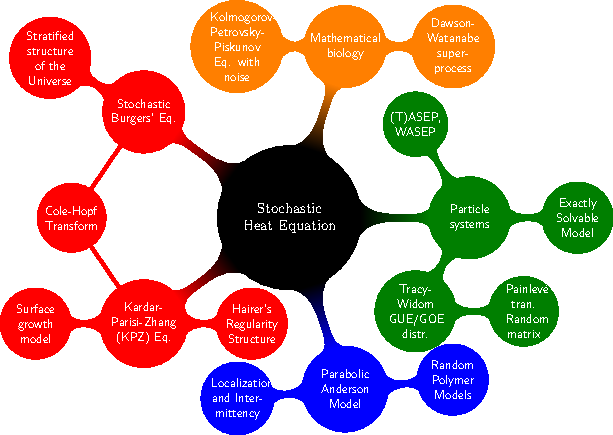
\includegraphics[scale=1.1]{figs/SHE_Mindmap2.pdf}
% \end{center}
\tikzset{
  set angles for level/.style={level #1/.append style={sibling angle=360/\the\tikznumberofchildren}},
  level/.append style={set angles for level=#1}}
\tikzset{level 1 concept/.append style={font=\sf, sibling angle=90,level distance = 25mm}}
\tikzset{level 2 concept/.append style={font=\sf, sibling angle=45,level distance = 15mm}}
\tikzset{level 3 concept/.append style={font=\sf, sibling angle=45,level distance = 15mm}}
\tikzset{every node/.append style={scale=0.6}}
 \tikzset{
    invisible/.style={opacity=0},
    visible on/.style={alt={#1{}{invisible} }},
    alt/.code args={<#1>#2#3}{%
      \alt<#1>{\pgfkeysalso{#2}}{\pgfkeysalso{#3}} % \pgfkeysalso doesn't change the path
    },
  }
\begin{center}
 \begin{tikzpicture}[scale=1.26]
  \path[mindmap,concept color=black,text=white]
    node[concept,visible on=<1->] {Stochastic\\ Heat Equation\\ $u(t,x)$}
    [clockwise from=0]
    child[concept color=green!50!black,visible on=<6->] {
      node[concept] {Particle systems} [clockwise from=120,sibling angle=30]
      child { node[concept] {(T)ASEP, \\ WASEP}
       }
       child { node[concept] {Exactly Solvable Model}}
       child { node[concept] {Tracy-Widom GUE/GOE distr. }[clockwise from=0,sibling angle=30]
       child { node[concept] {Painlev\'e tran.\\
       Random matrix}}
       }
    }
    child[concept color=blue,visible on=<7->] {
      node[concept] {Parabolic Anderson Model}
      [clockwise from=5]
      child { node[concept] {Random Polymer Models} }
      child { node[concept] {Localization and Intermittency} }
    }
    child[concept color=red,visible on=<2->] { node[concept] (KPZ) {Kardar-Parisi-Zhang (KPZ) Eq.}
    [clockwise from=180,sibling angle=-90]
    child { node[concept] {Surface growth model} }
    child { node[concept] {Hairer's Regularity Structure} }
    }
    child[concept color=red,visible on=<3->] { node[concept] (Burgers) {Stochastic Burgers' Eq.}
    [clockwise from=150]
    child { node[concept] {Stratified structure of the Universe} }}
    child[concept color=orange,visible on=<5->] { node[concept] {Mathematical biology}[clockwise from=0]
    child { node[concept] { Dawson-Watanabe superprocess}}
    child { node[concept] {Kolmogorov-Petrovsky-Piskunov Eq. with noise}}
    };
  \node[circle,extra concept,text=white,concept color=red,visible on=<4->] (additional) at ($(Burgers)!0.5!(KPZ)+(-1,0)$) {Cole-Hopf \\Transform\\
  $\log u(t,x)$};
  \draw[ultra thick,red,visible on=<4->] (additional) -- (KPZ);
  \draw[ultra thick,red,visible on=<4->] (additional) -- (Burgers);
\end{tikzpicture}
\end{center}
\end{frame}
% }}}
% {{{ 4.
\begin{frame}
\[\left(\displaystyle\frac{\partial}{\partial t}
-\frac{1}{2}\Delta \right) u(t,x) =
\rho(u(t,x))  \dot{W}(t,x)\]
\vspace{-1.8em}
 \begin{center}
  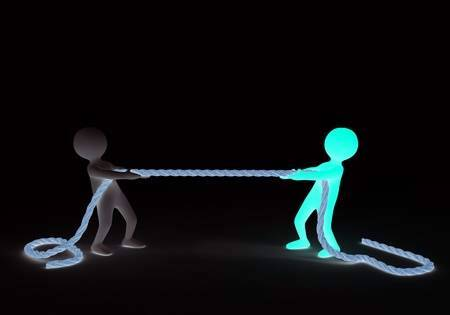
\includegraphics[scale=0.35]{figs/picture-tug-war2-neg.jpg}
  \vfill
  \begin{tabular}{ c c c  }
%   \hline
   $\Delta$ &  & $\rho(u)\dot{W}$ \\[0.5em]
   \hline\\
  Smoothing &  & Roughening \\
%   \hline
\end{tabular}
 \end{center}
\end{frame}
% }}}
% {{{ 5.
\begin{frame}
  \frametitle{\small
  $\left(\frac{\partial}{\partial t}-\frac{\partial^2}{\partial x^2}\right)u(t,x)=\lambda u(t,x) \W(t,x)$,
  $x\in [-	1/2,1/2]$ with $u(0,x)=\cos(\pi x)$\\
  \visible<3->{Bearded SHE}}
  \pause
  \centering
  \visible<2->{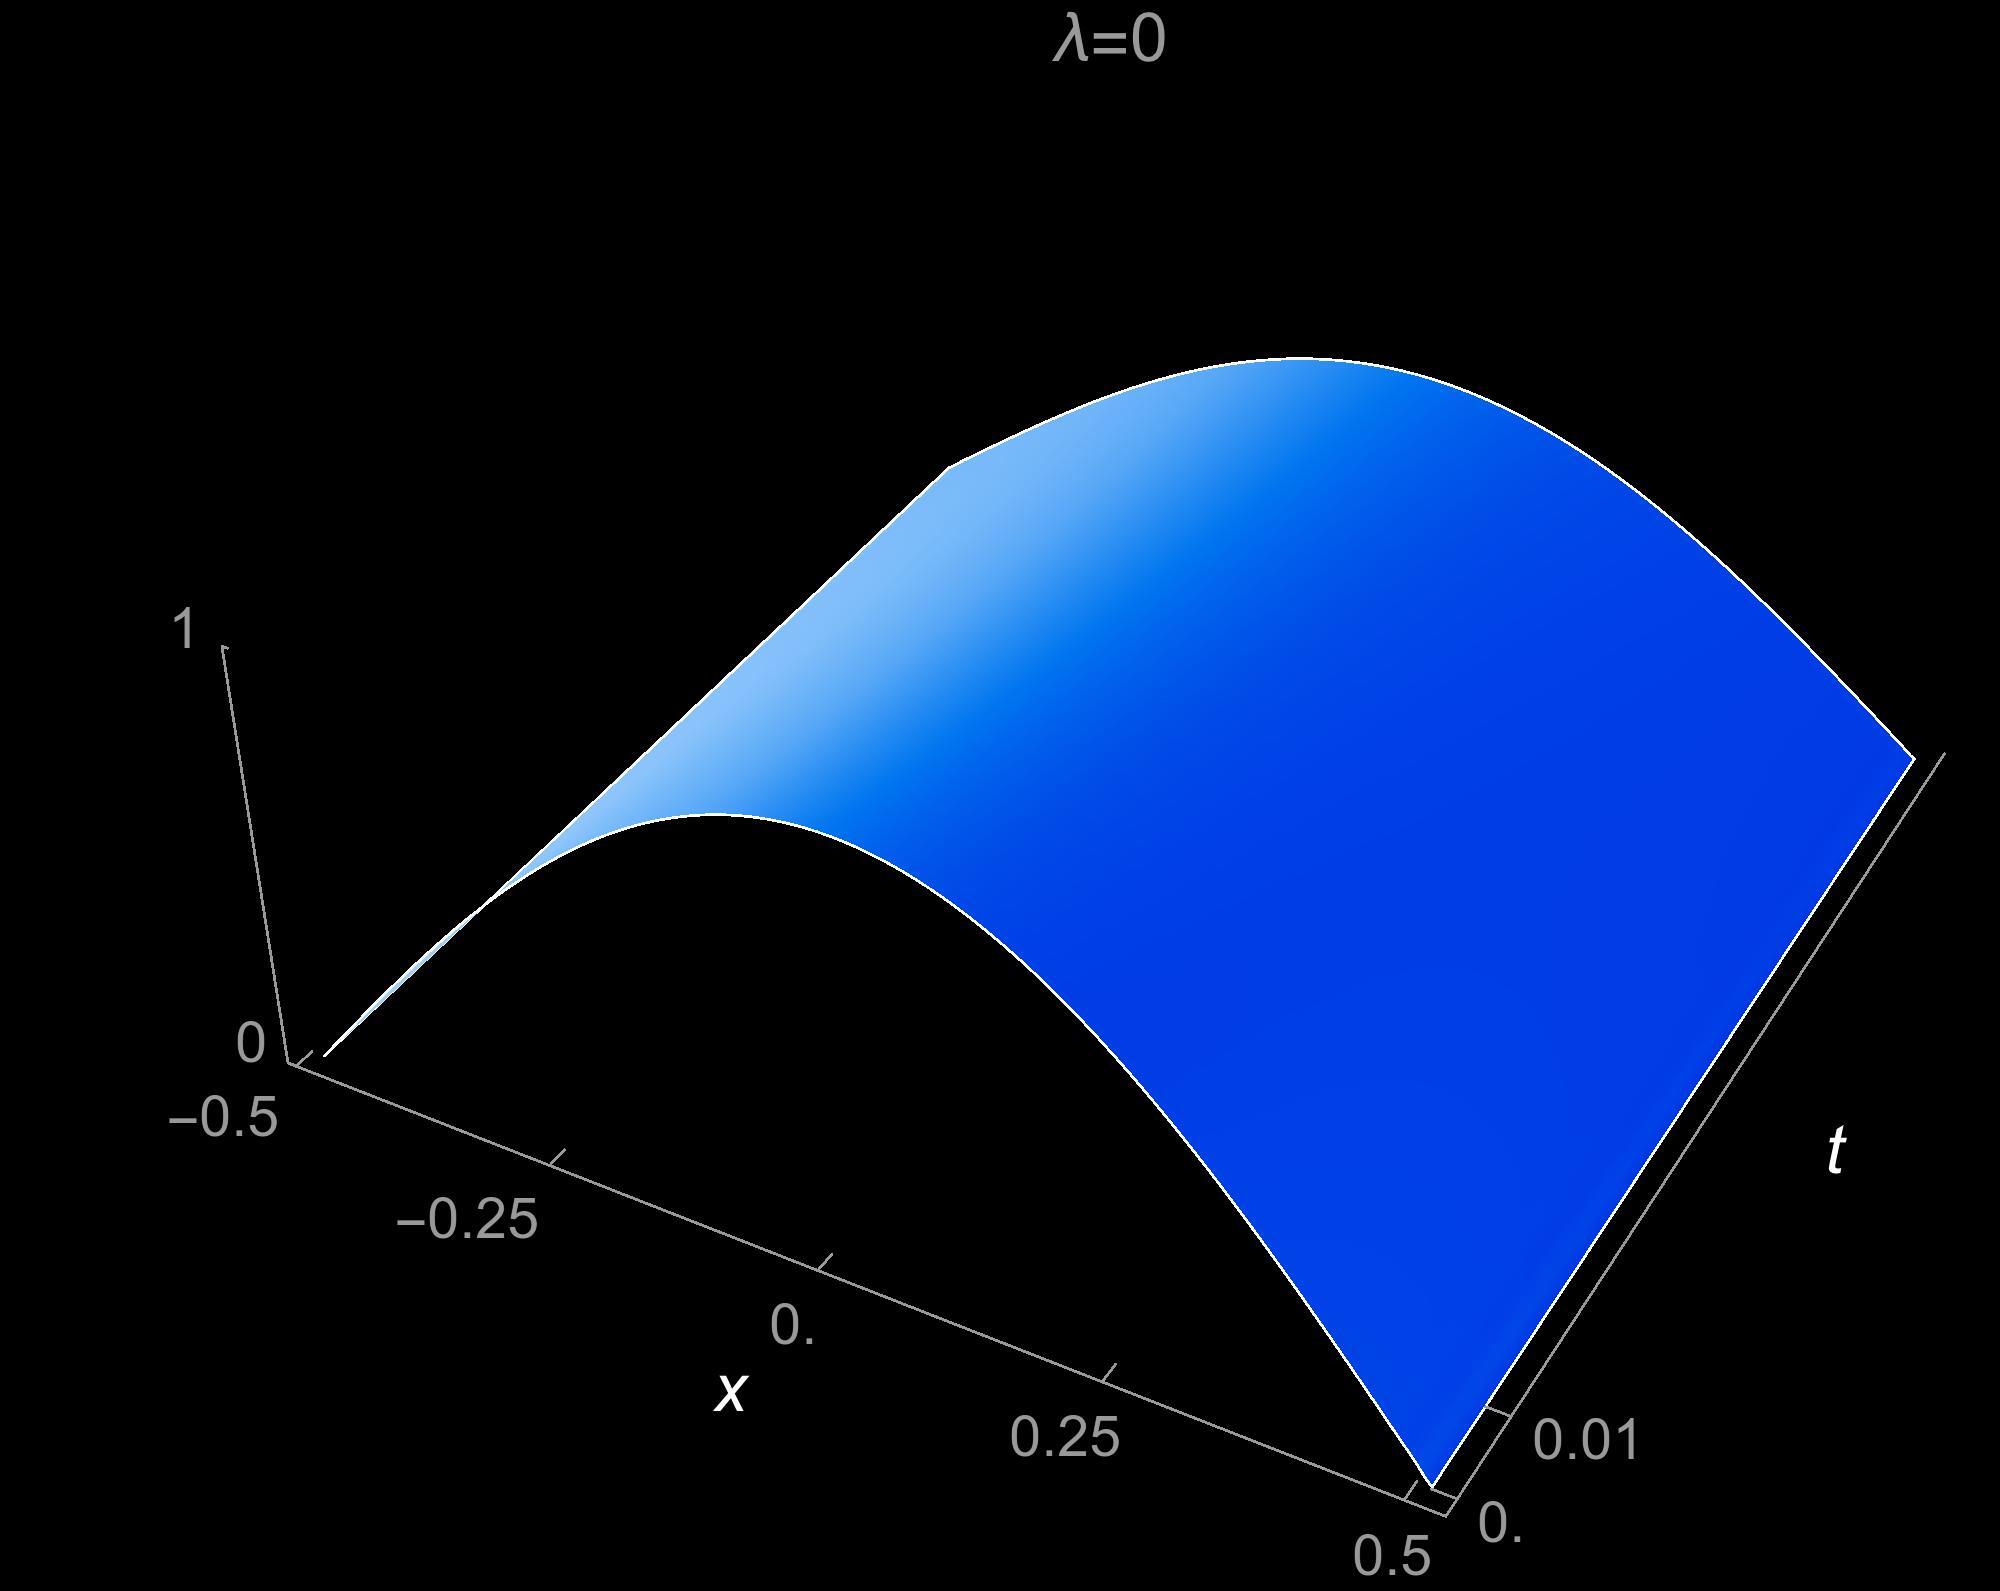
\includegraphics[scale=0.06]{figs/Sin_L0-neg.jpeg}}
  \quad
  \pause
  \visible<3->{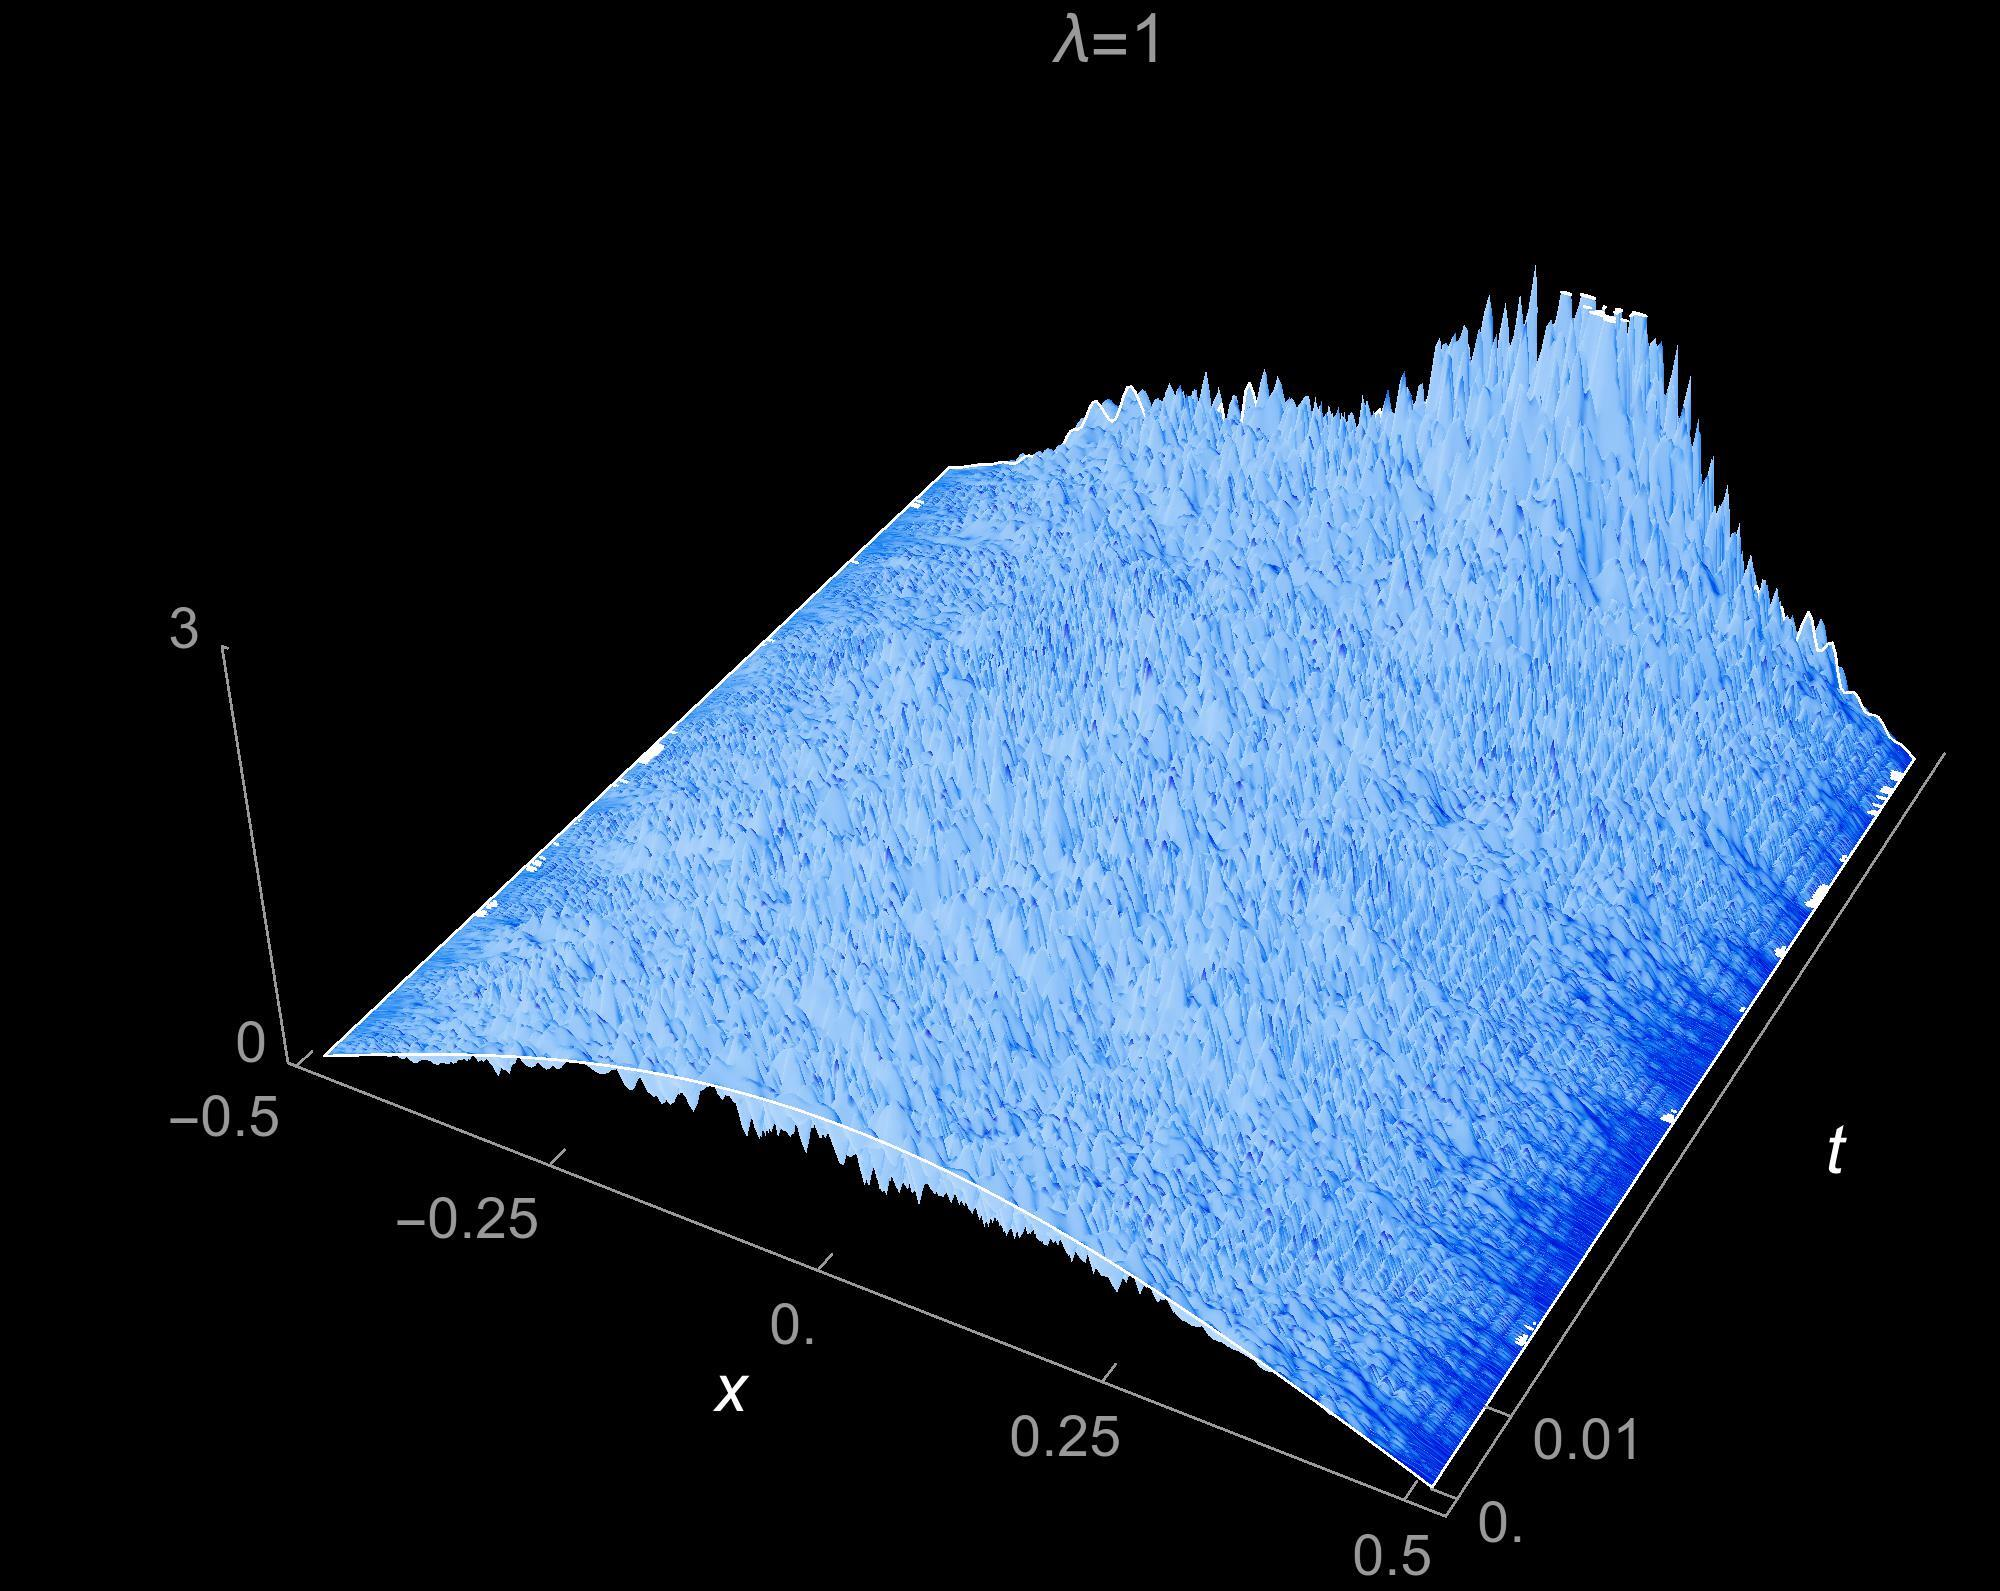
\includegraphics[scale=0.06]{figs/Sin_L1-neg.jpeg}}\\
  \pause
  \visible<4->{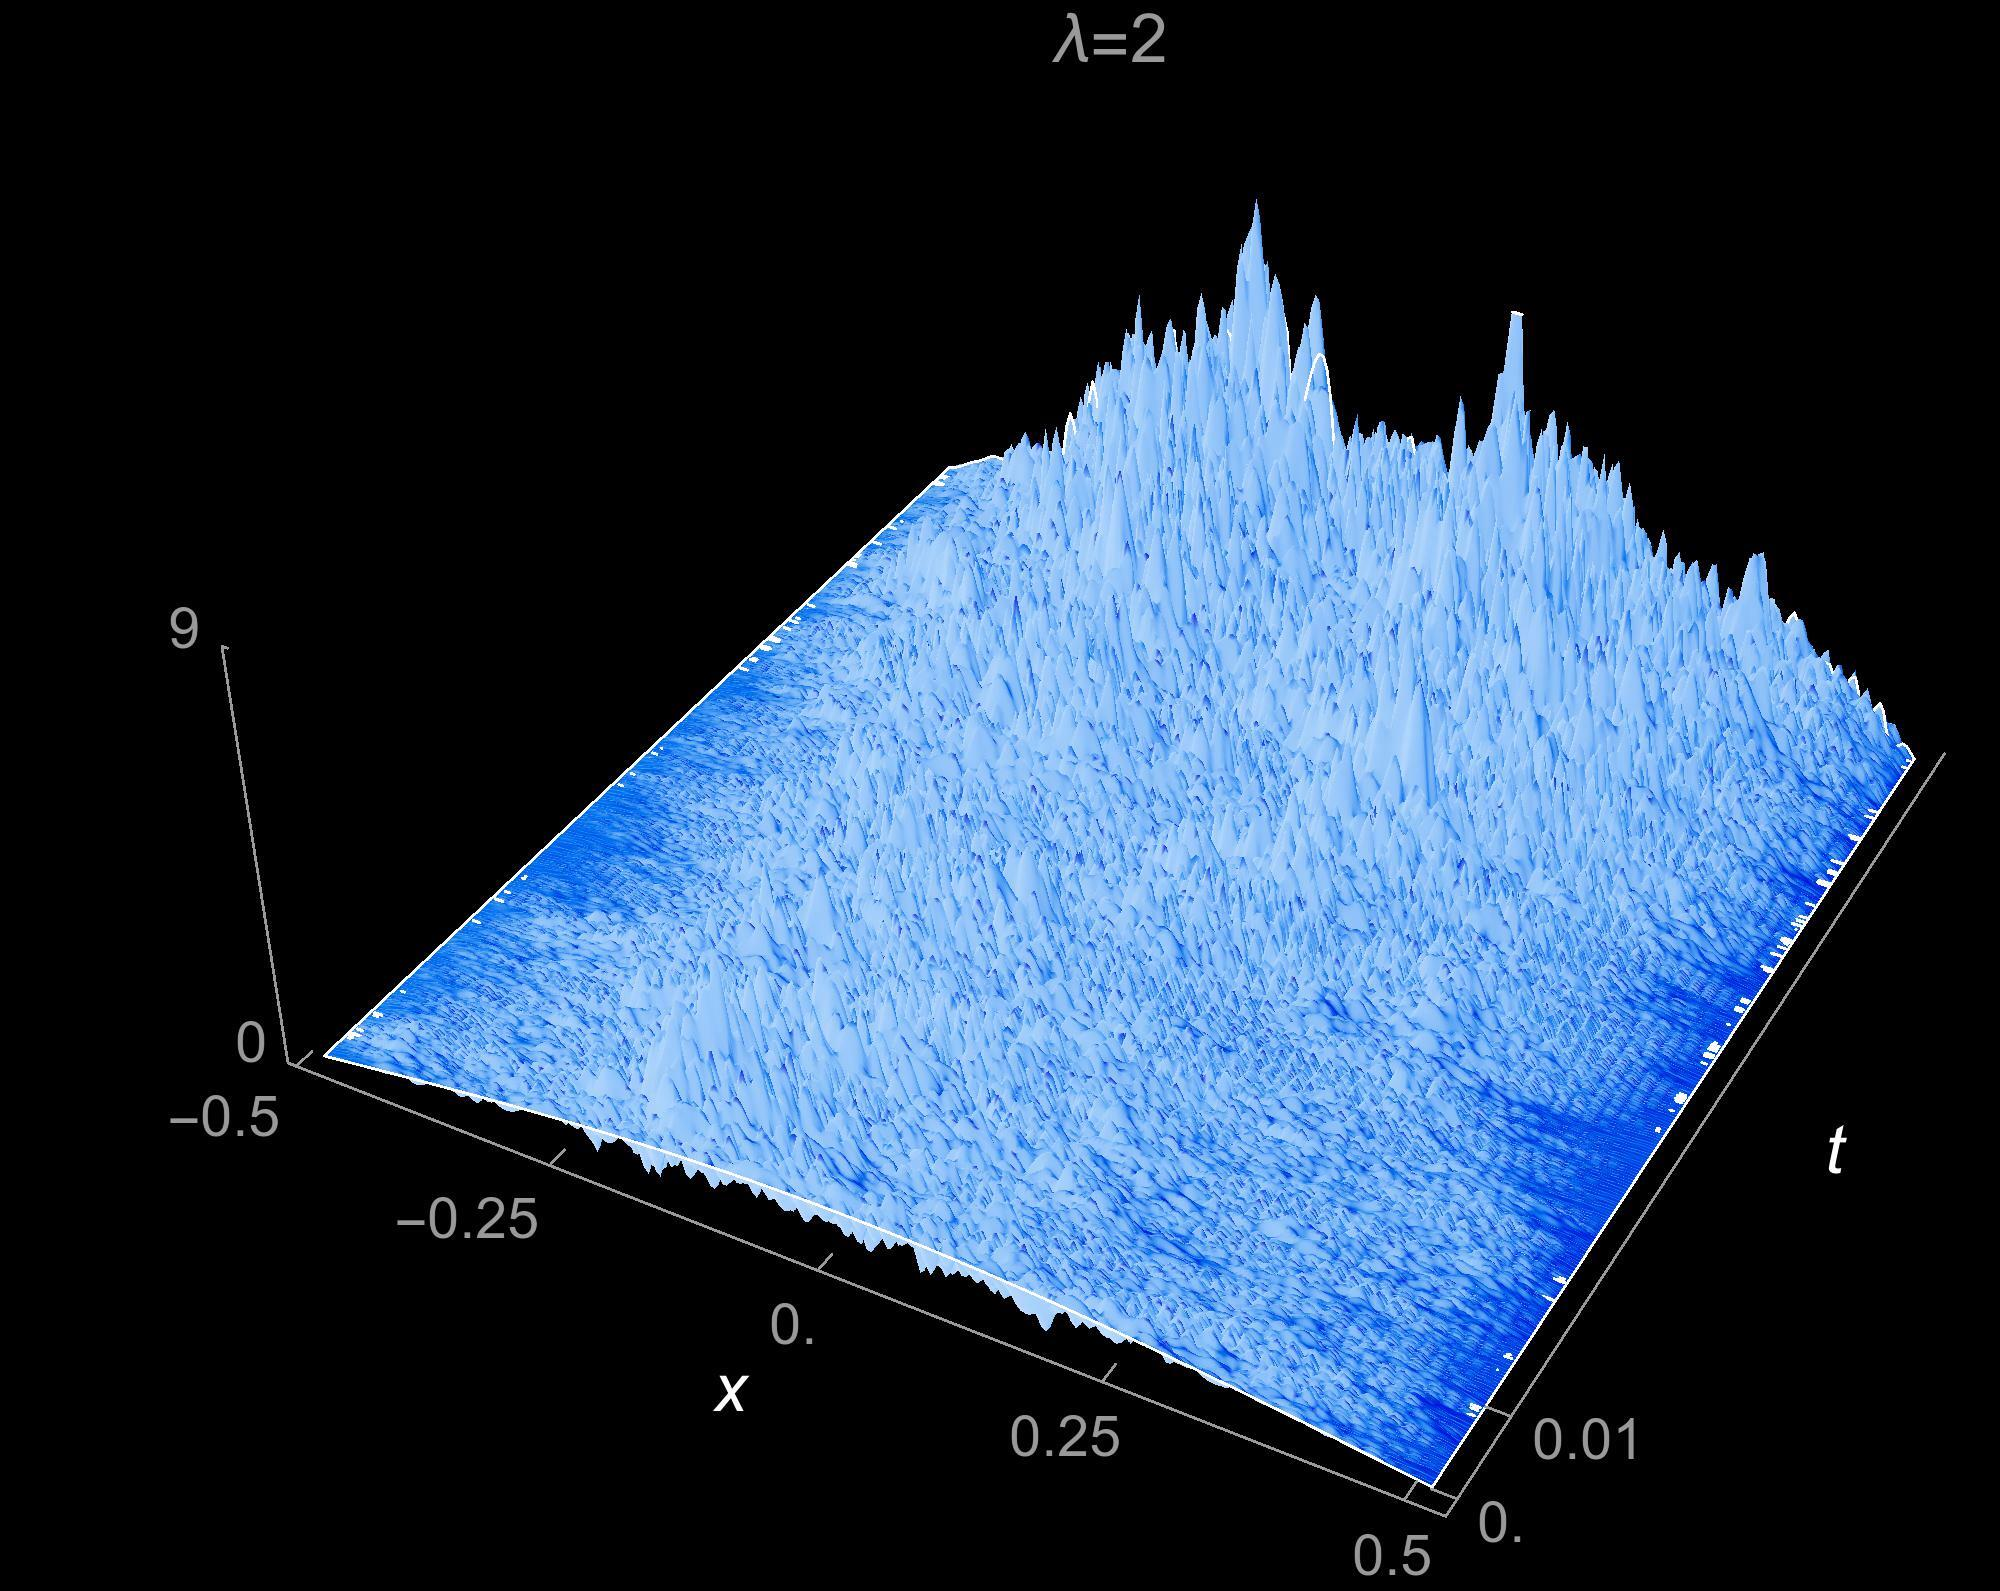
\includegraphics[scale=0.06]{figs/Sin_L2-neg.jpeg}}
  \quad
  \pause
  \visible<5->{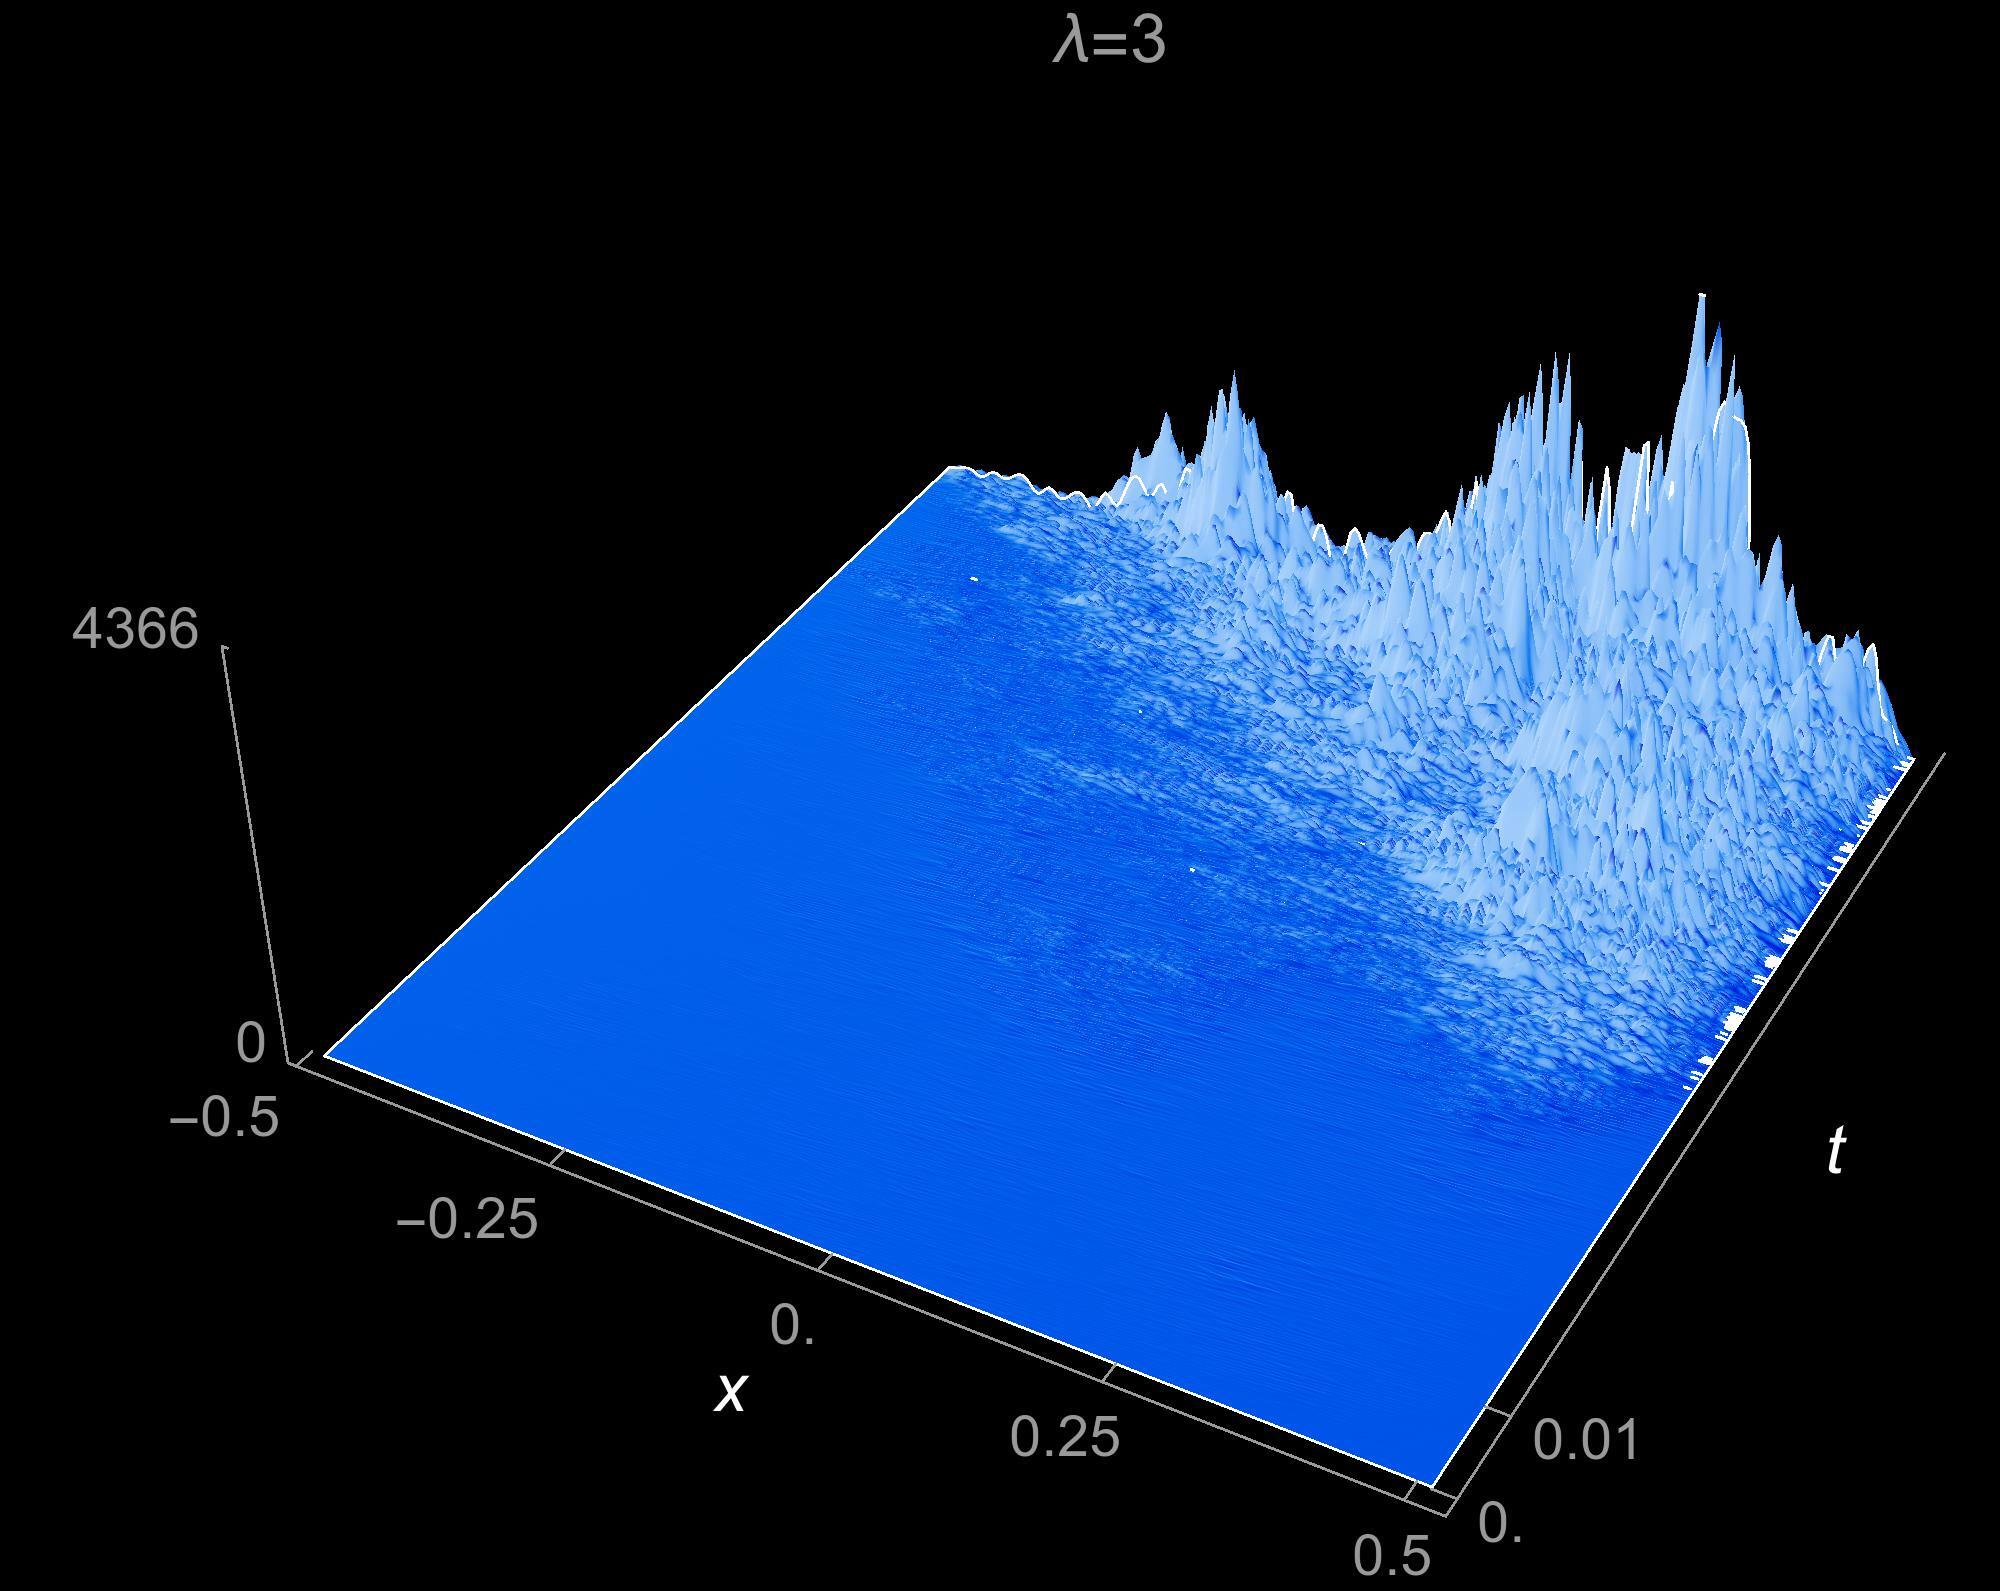
\includegraphics[scale=0.06]{figs/Sin_L3-neg.jpeg}}
\end{frame}
% }}}
% {{{ 6.
\begin{frame}
  \frametitle{\vspace{0.5em}
  $\left(\frac{\partial}{\partial t}-\frac{\partial^2}{\partial x^2}\right)u(t,x)=\lambda u(t,x) \W(t,x)$,
  $x\in\R$ \\[0.5em] \small
  with localized initial data}
  \small
  \centering
  \only<2-7>{
    \visible<2-7>{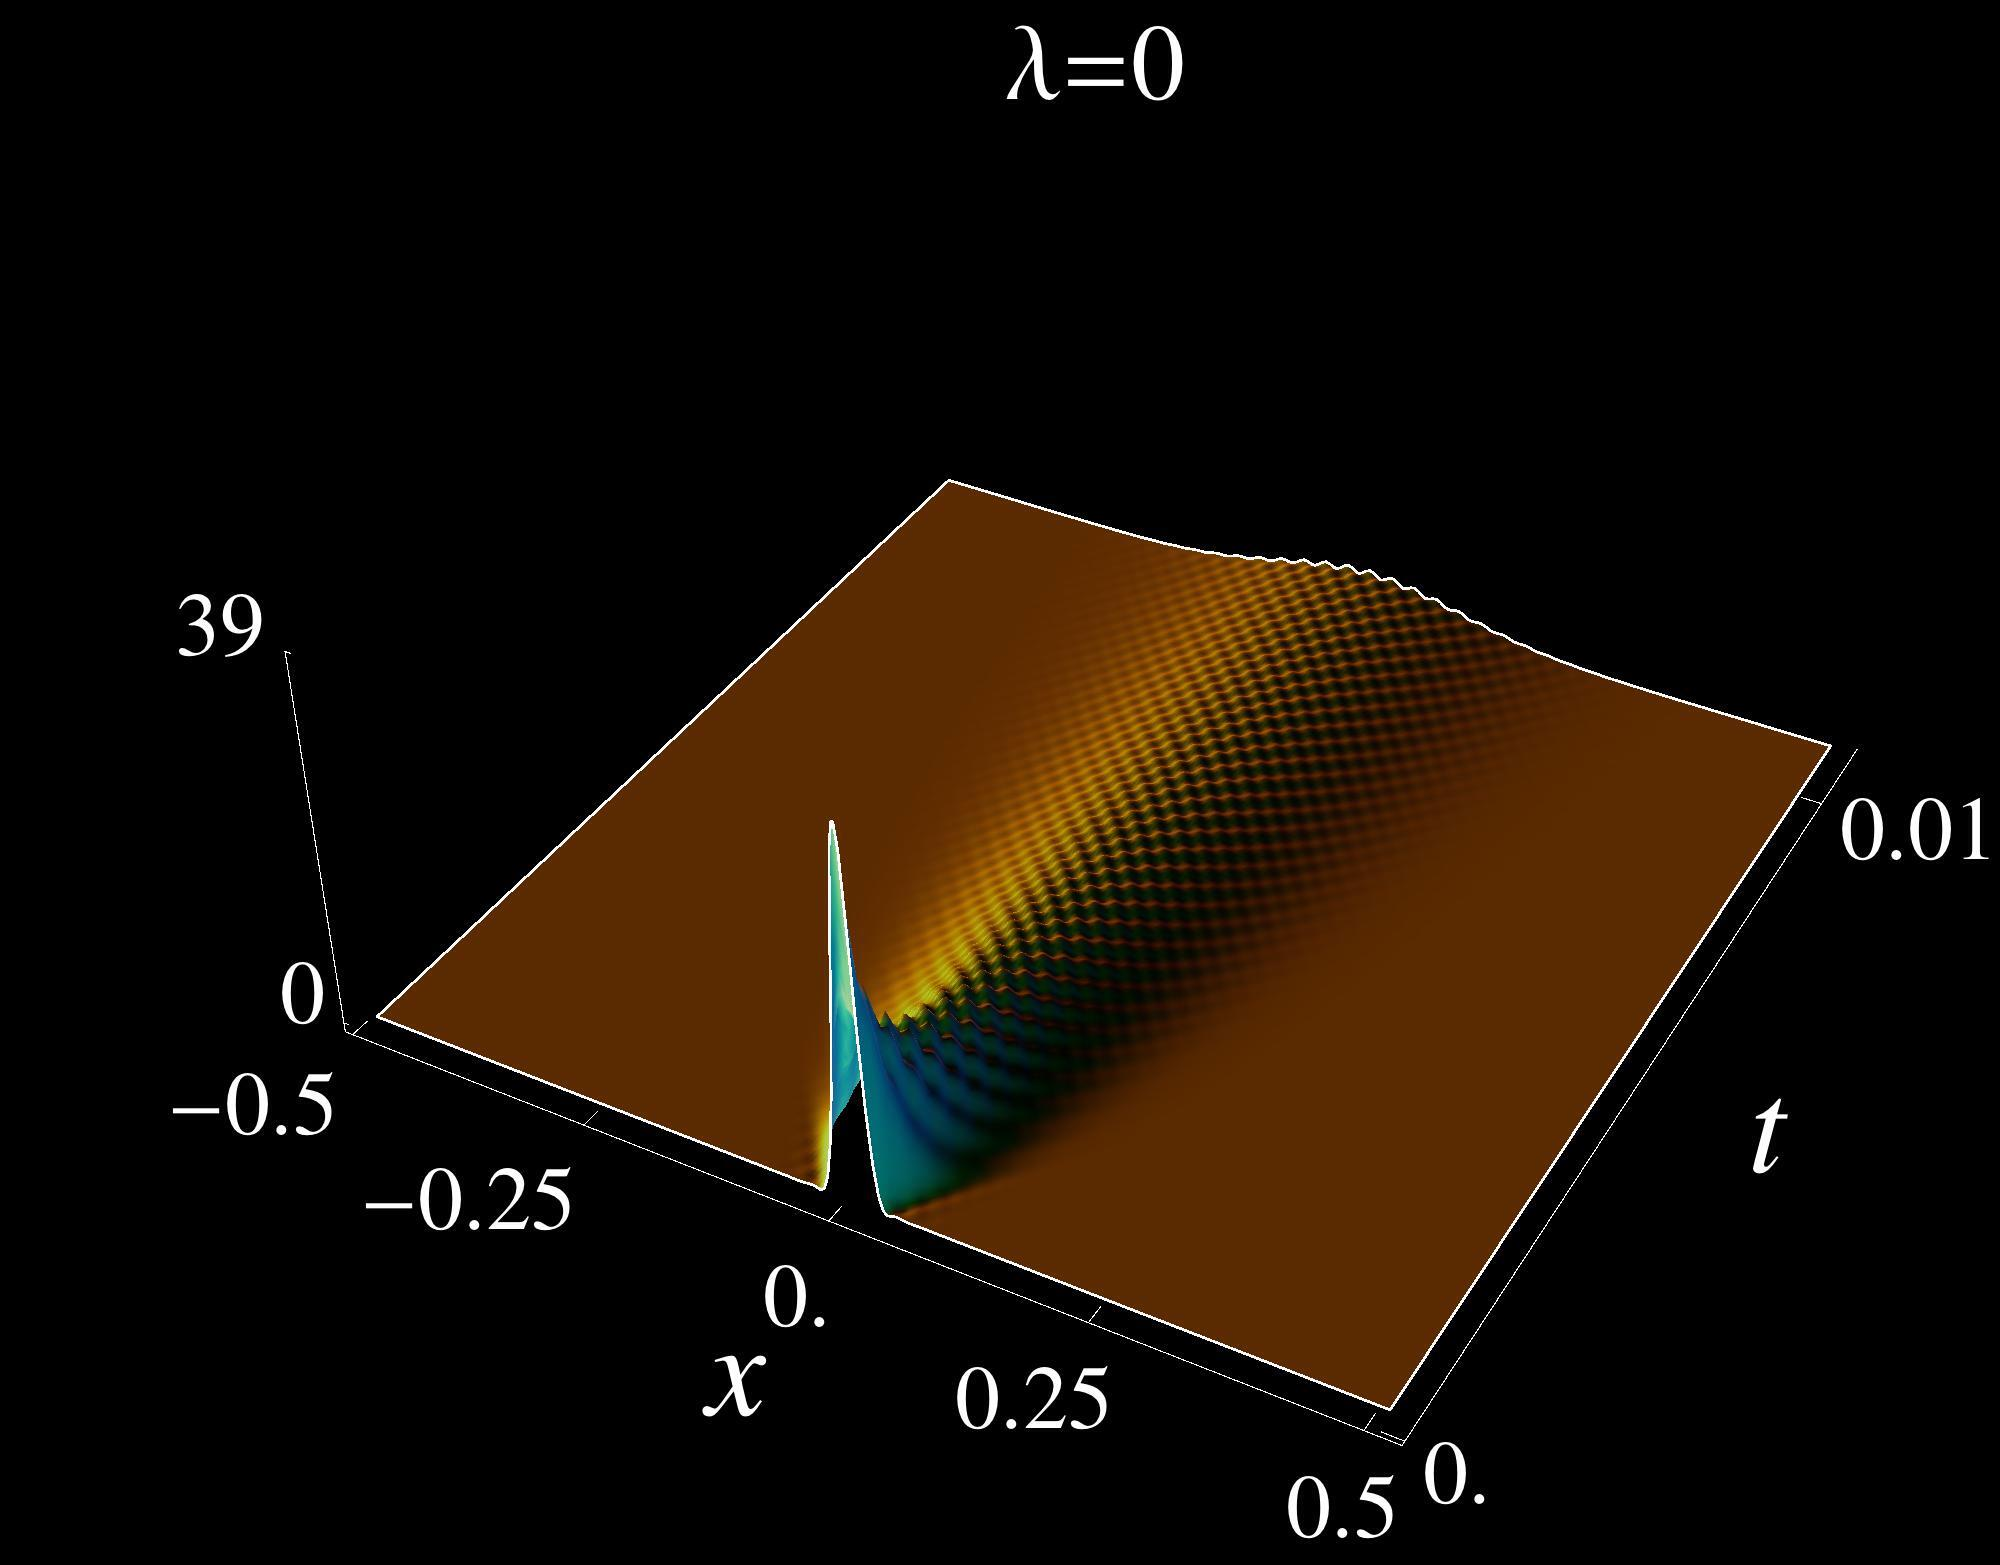
\includegraphics[scale=0.05]{figs/small_Delta_L0-neg.jpeg}}
    \visible<3-7>{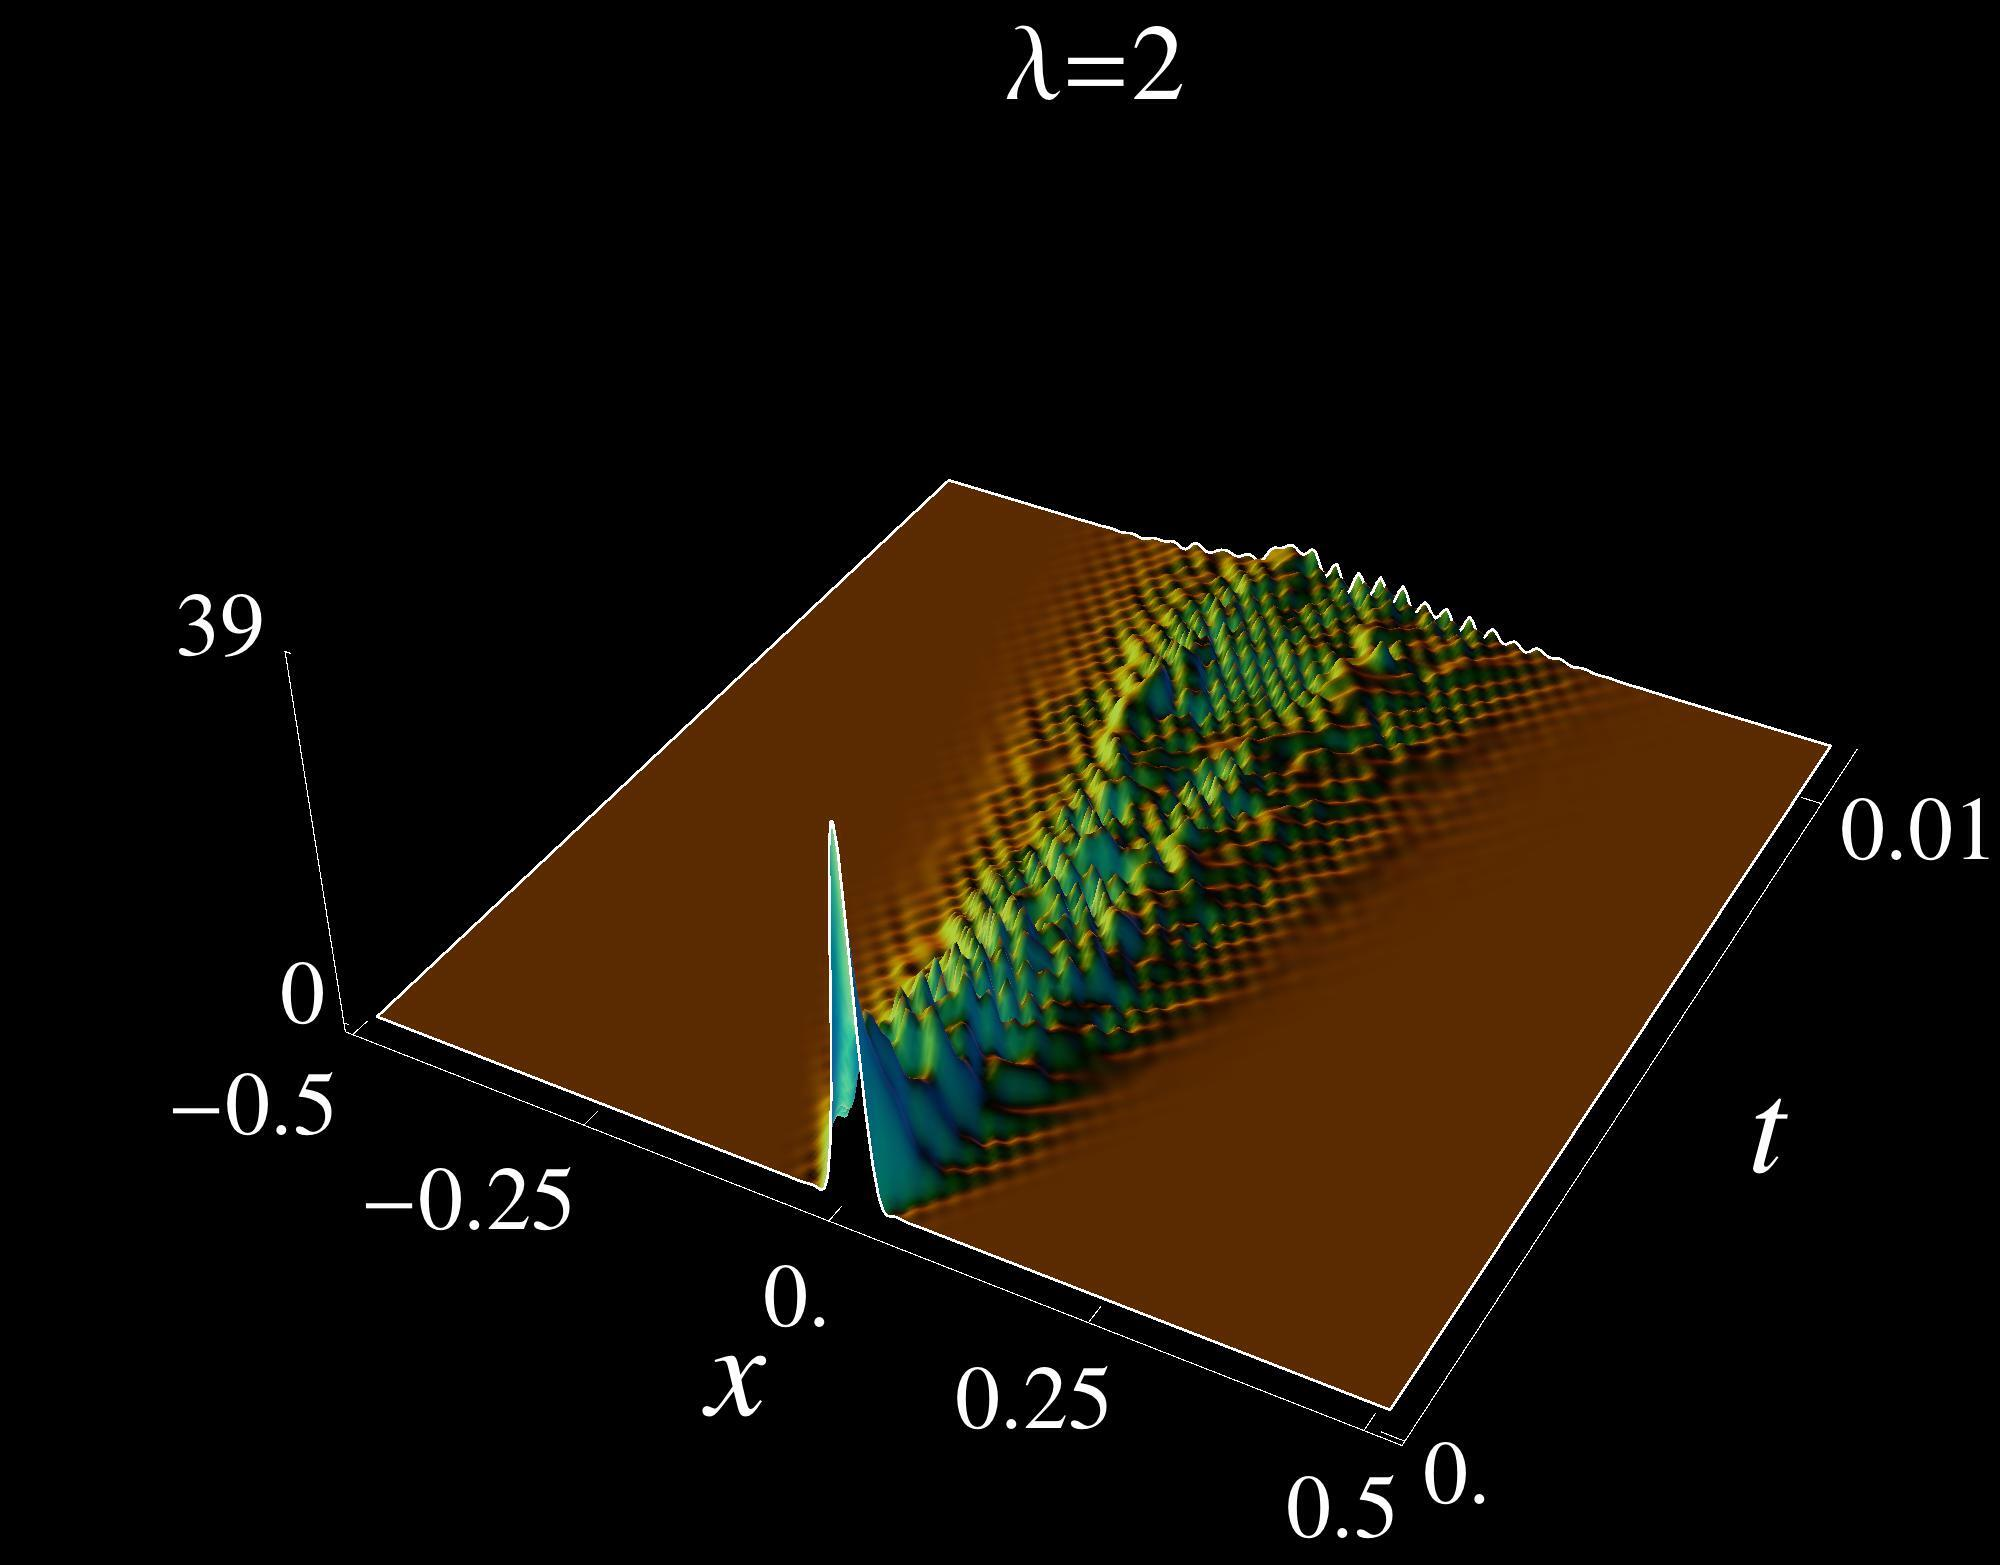
\includegraphics[scale=0.05]{figs/small_Delta_L2-neg.jpeg}}
    \visible<4-7>{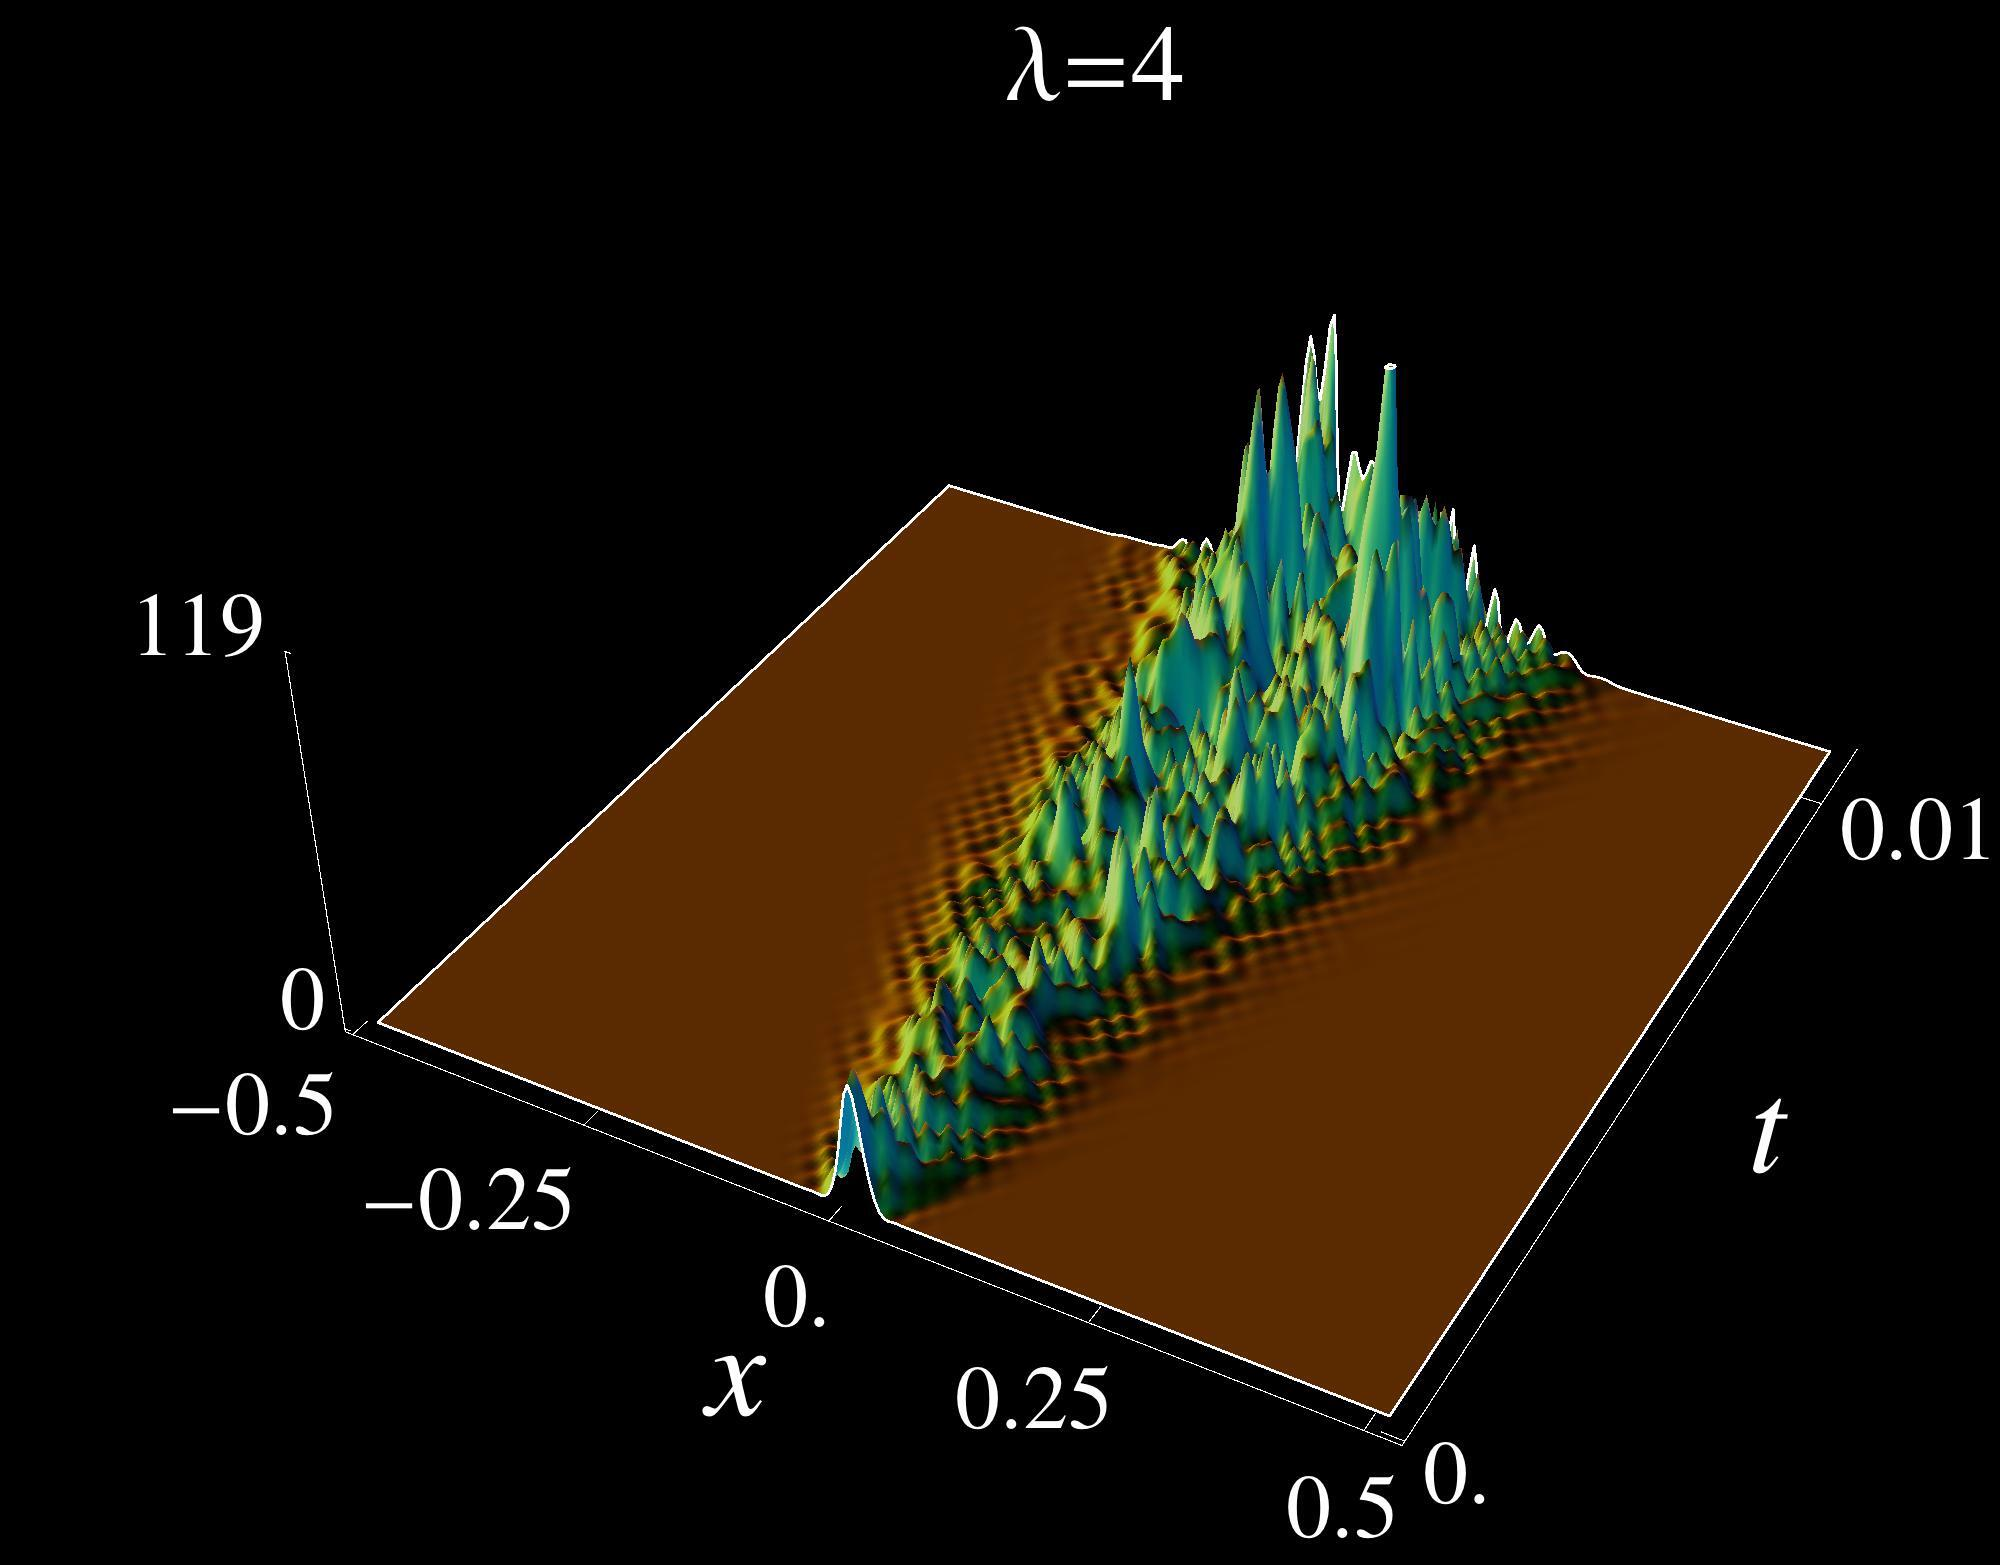
\includegraphics[scale=0.05]{figs/small_Delta_L4-neg.jpeg}}\\ \vfill
    \visible<5-7>{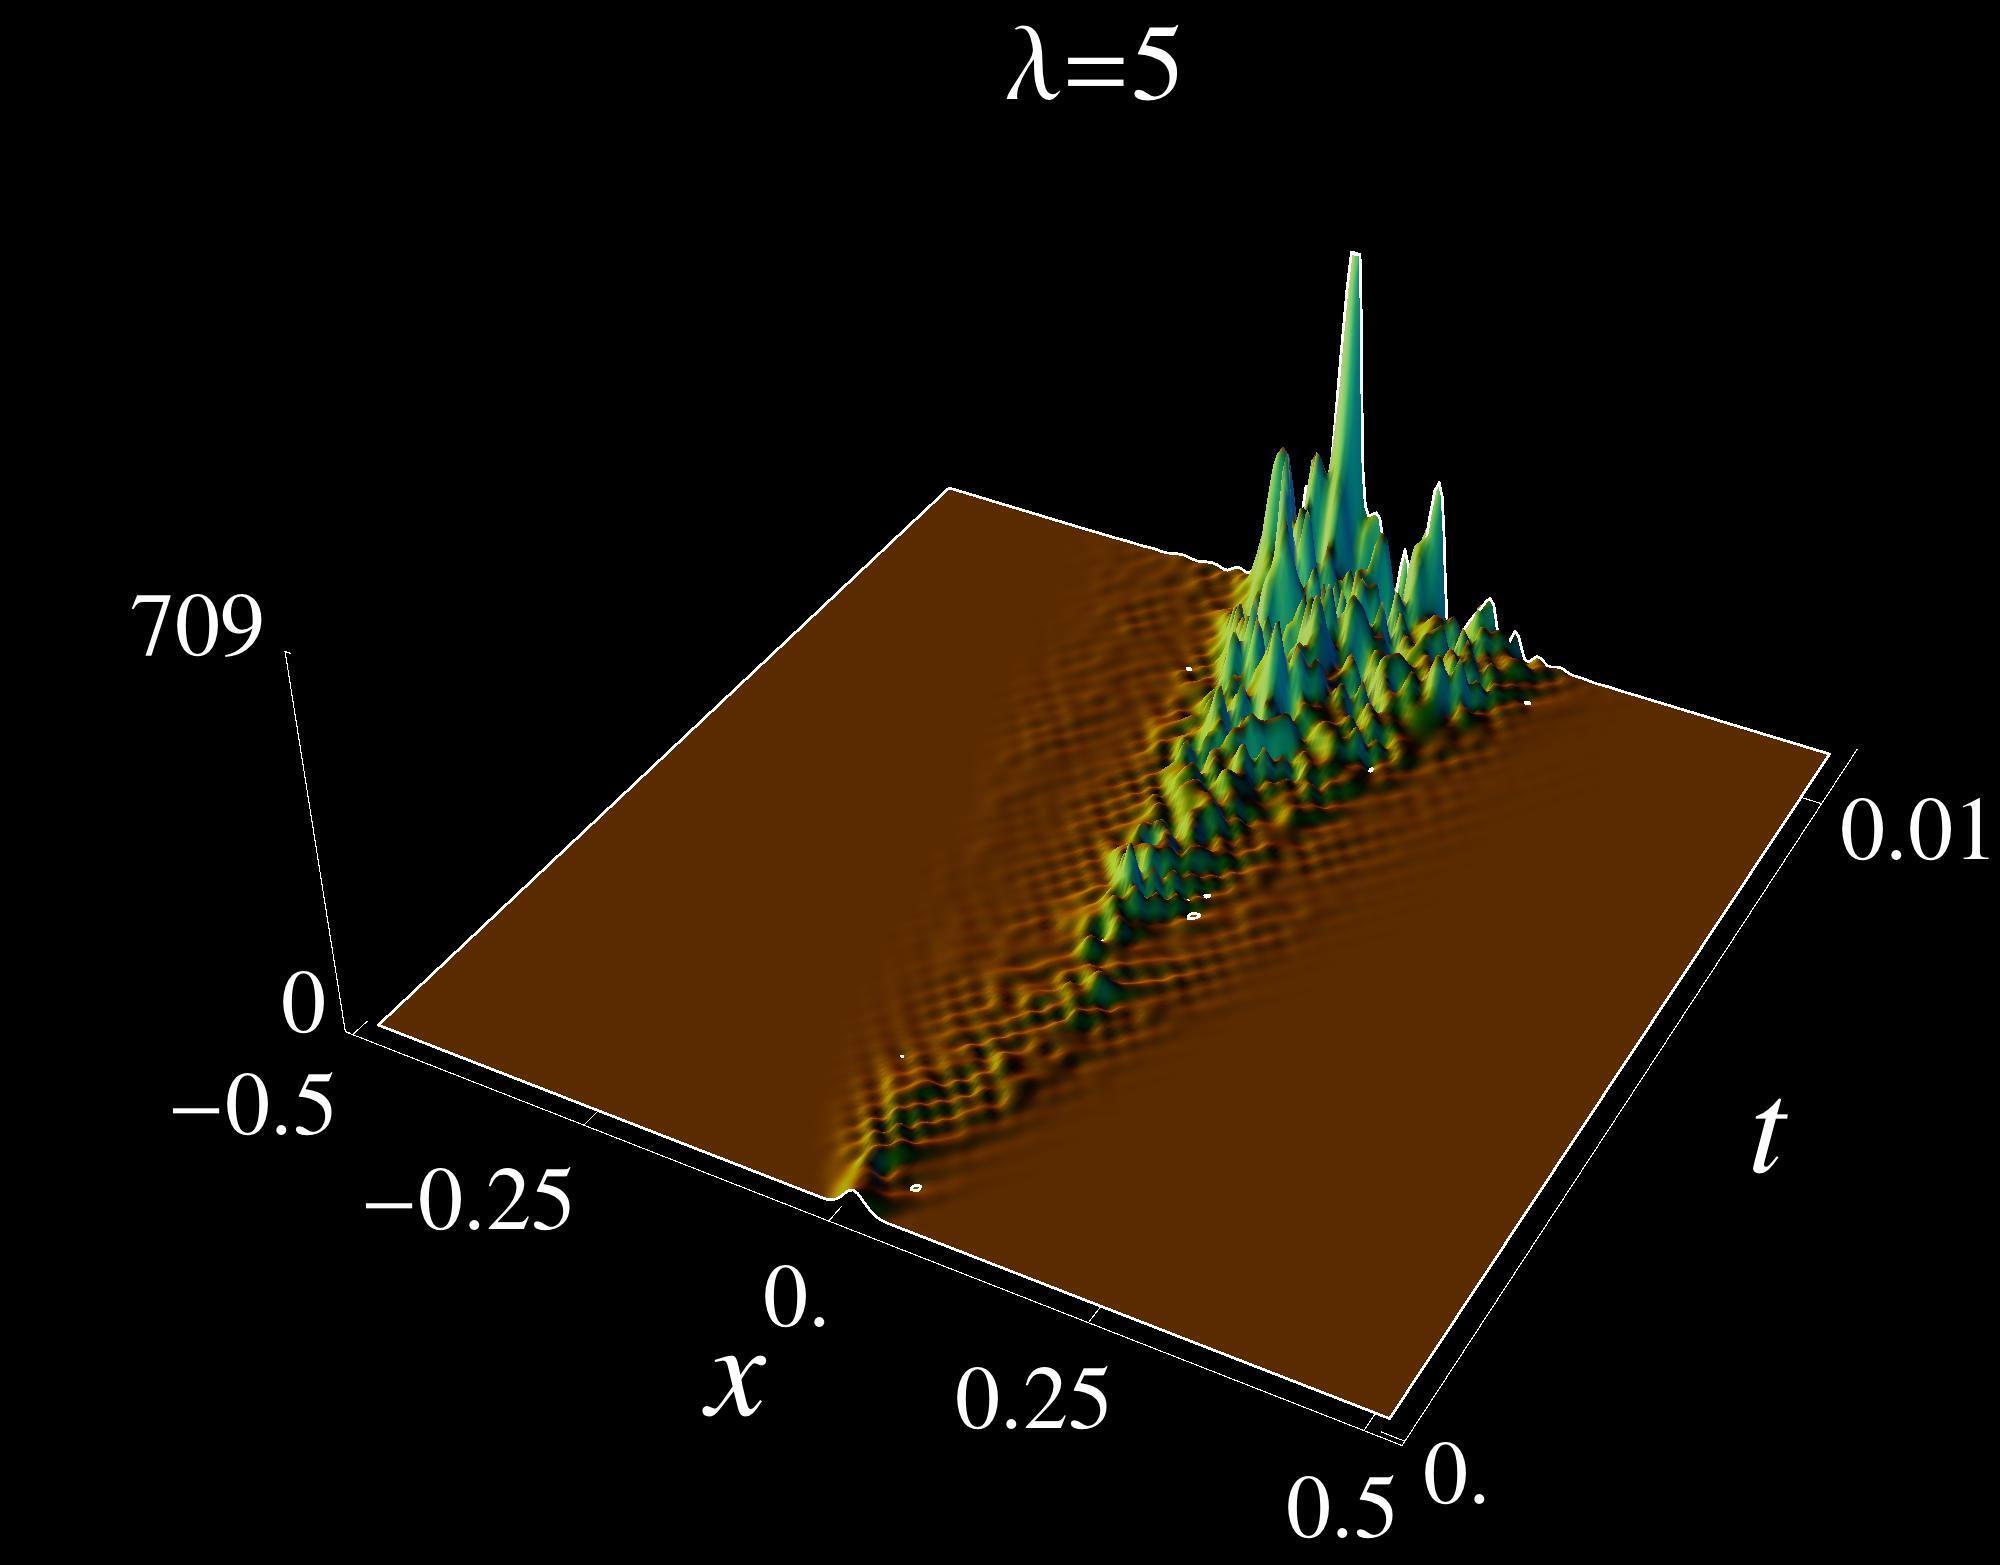
\includegraphics[scale=0.05]{figs/small_Delta_L5-neg.jpeg}}
    \visible<6-7>{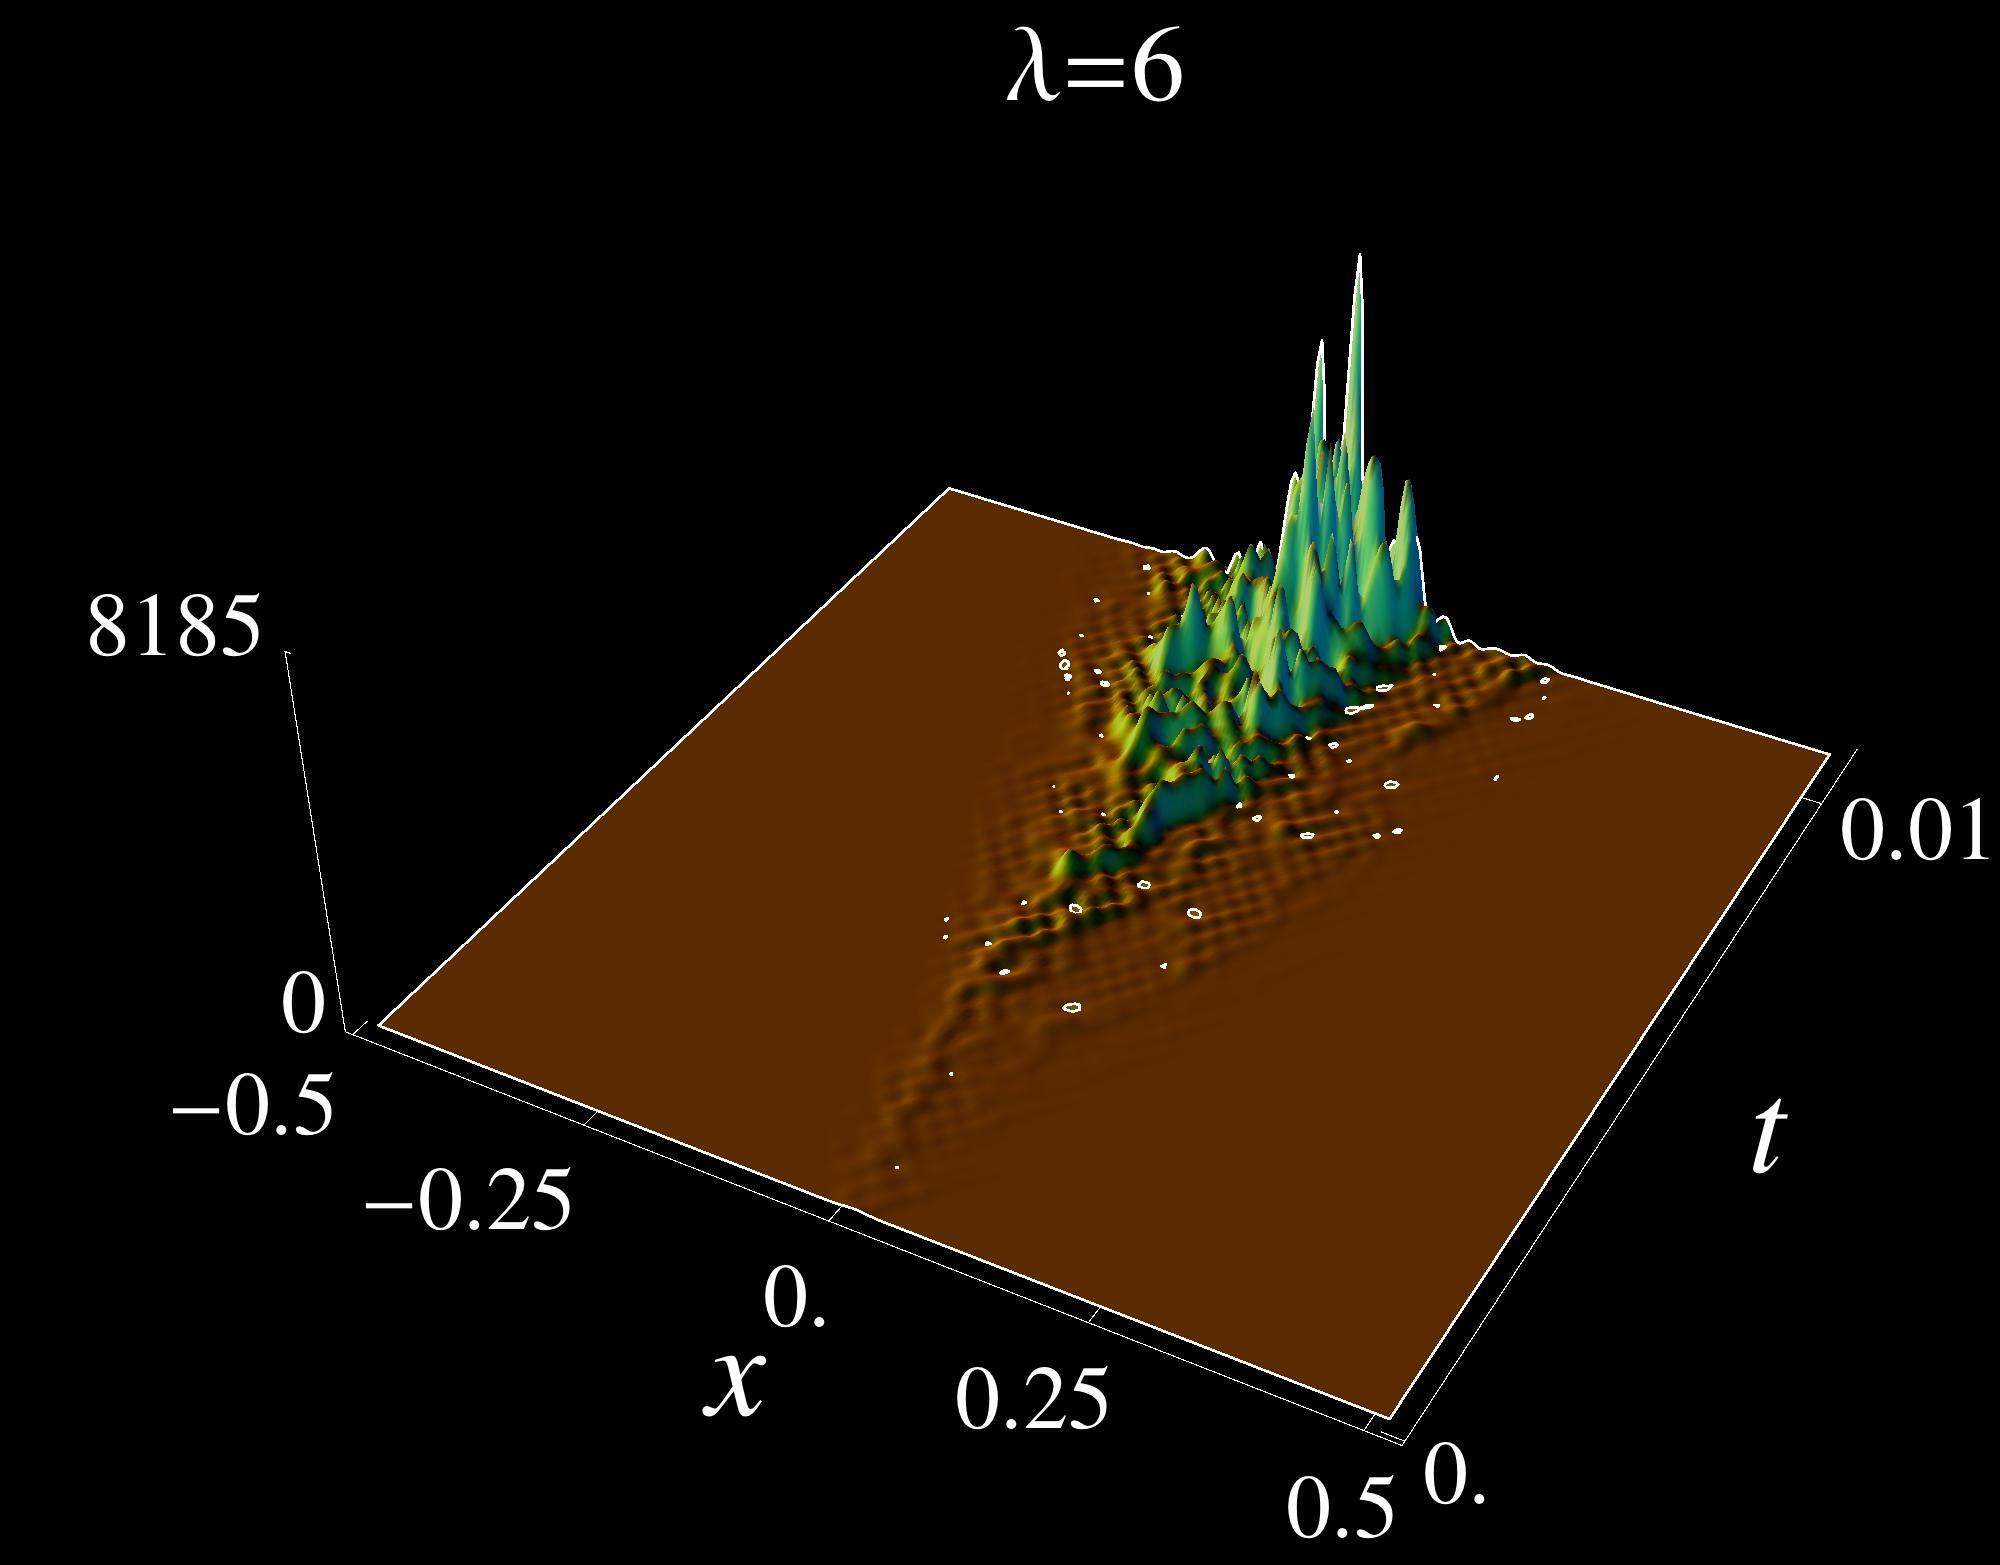
\includegraphics[scale=0.05]{figs/small_Delta_L6-neg.jpeg}}
    \visible<7>{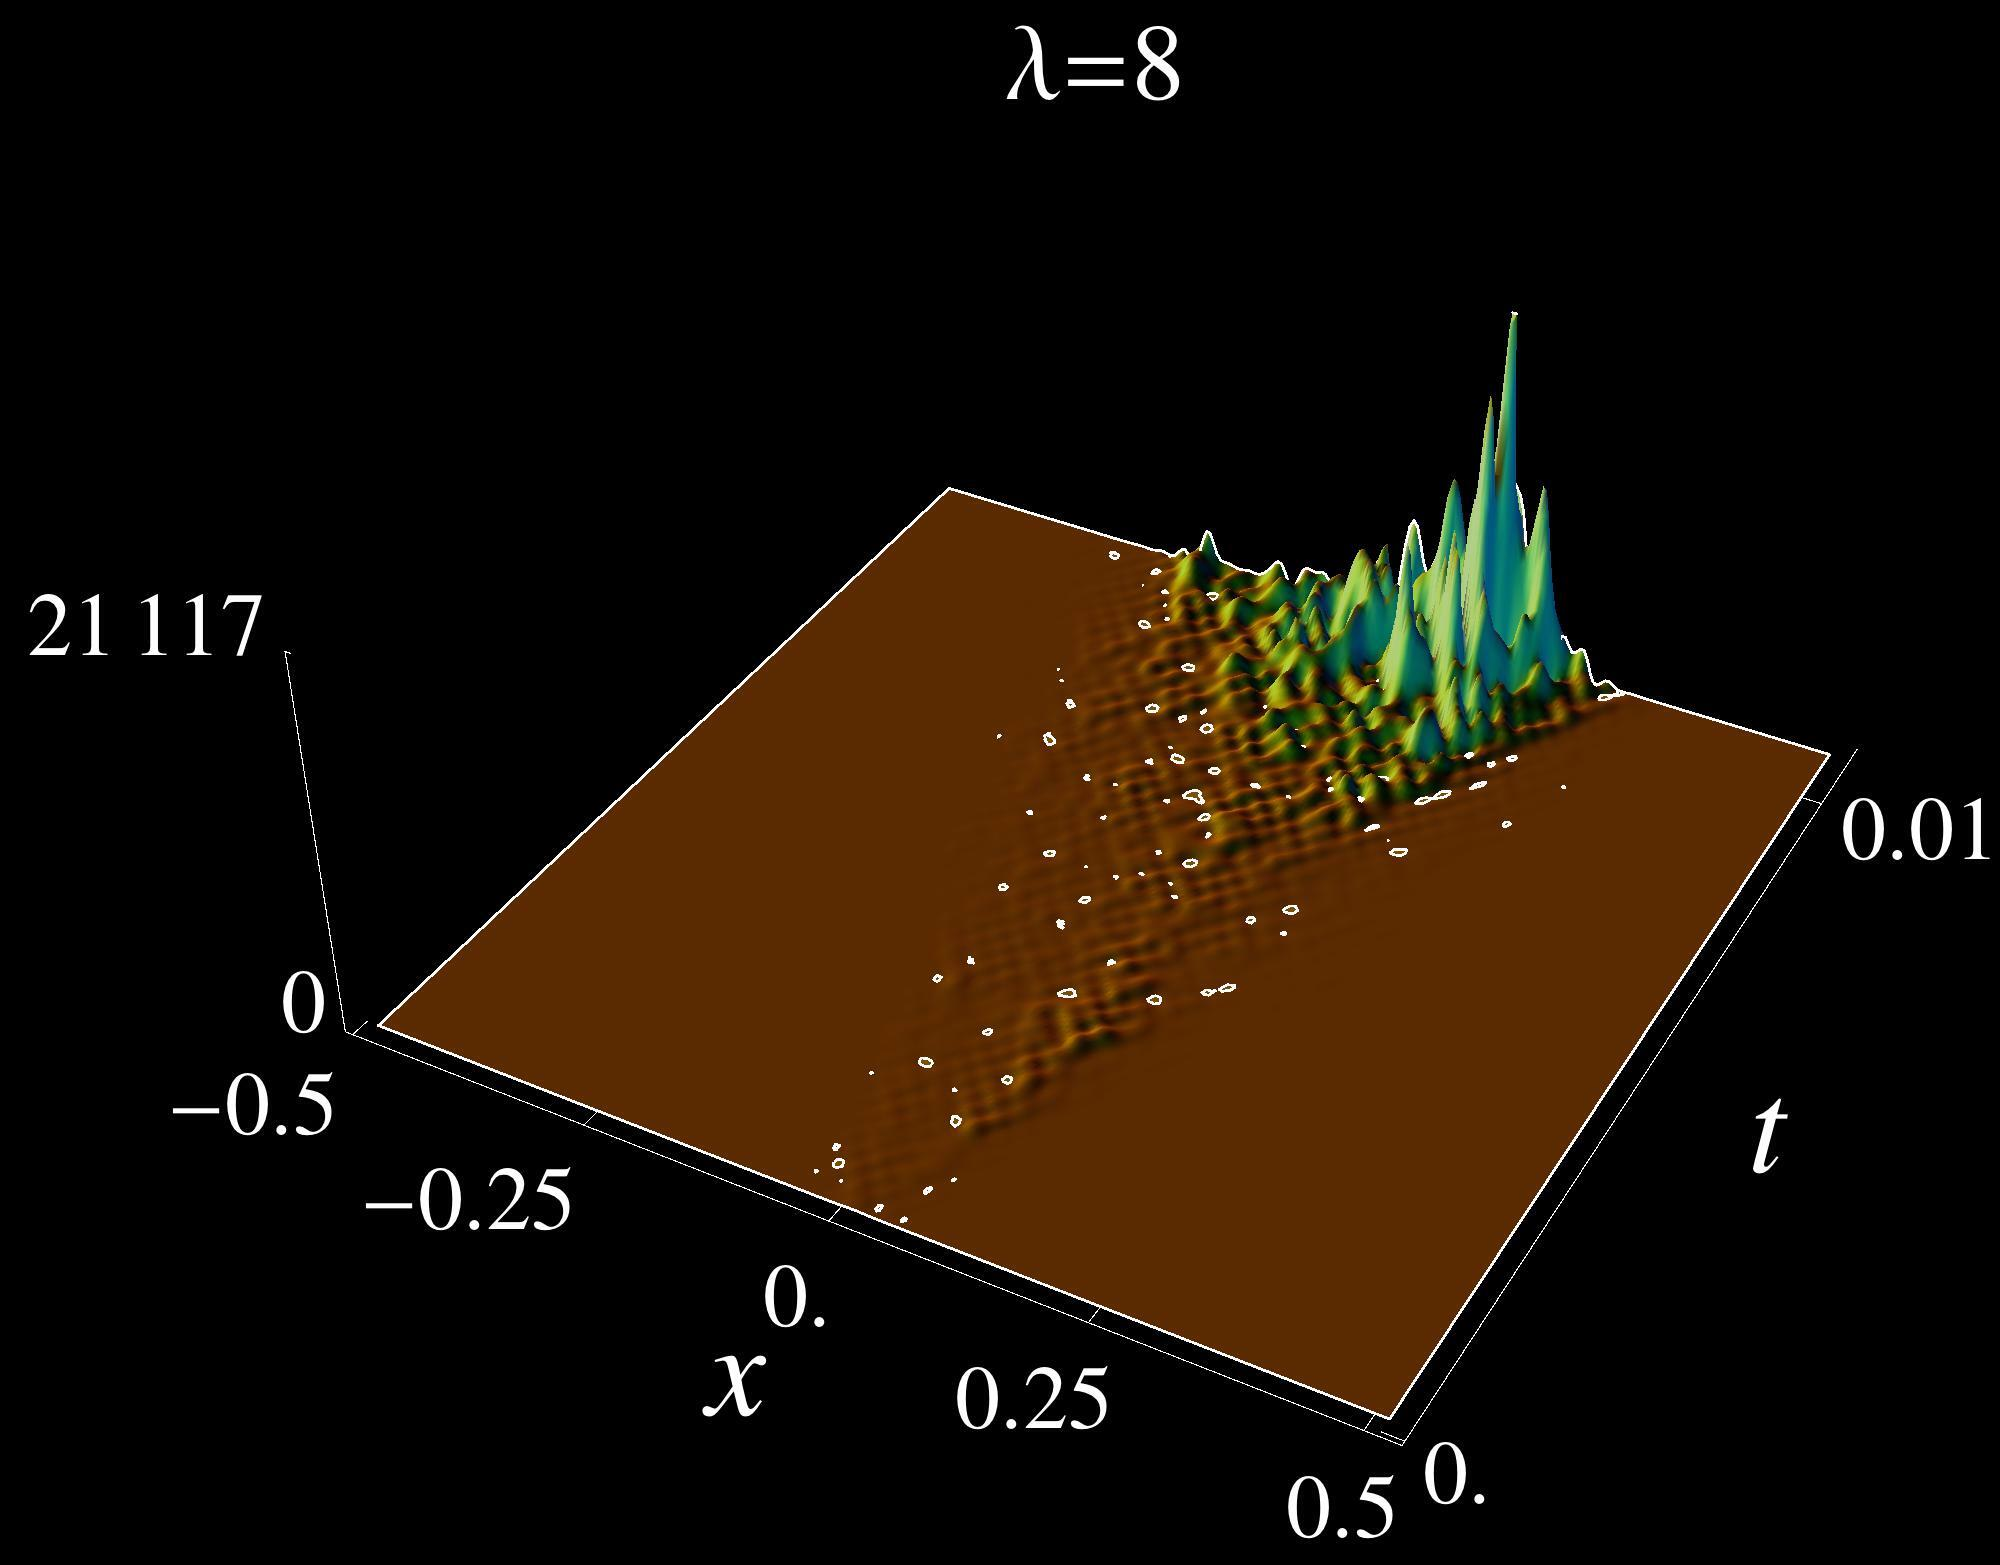
\includegraphics[scale=0.05]{figs/small_Delta_L8-neg.jpeg}}\\
    \phantom{aaa}\\[3.3em]
    \phantom{aaaaaa}
    }
  \only<8-9>{
    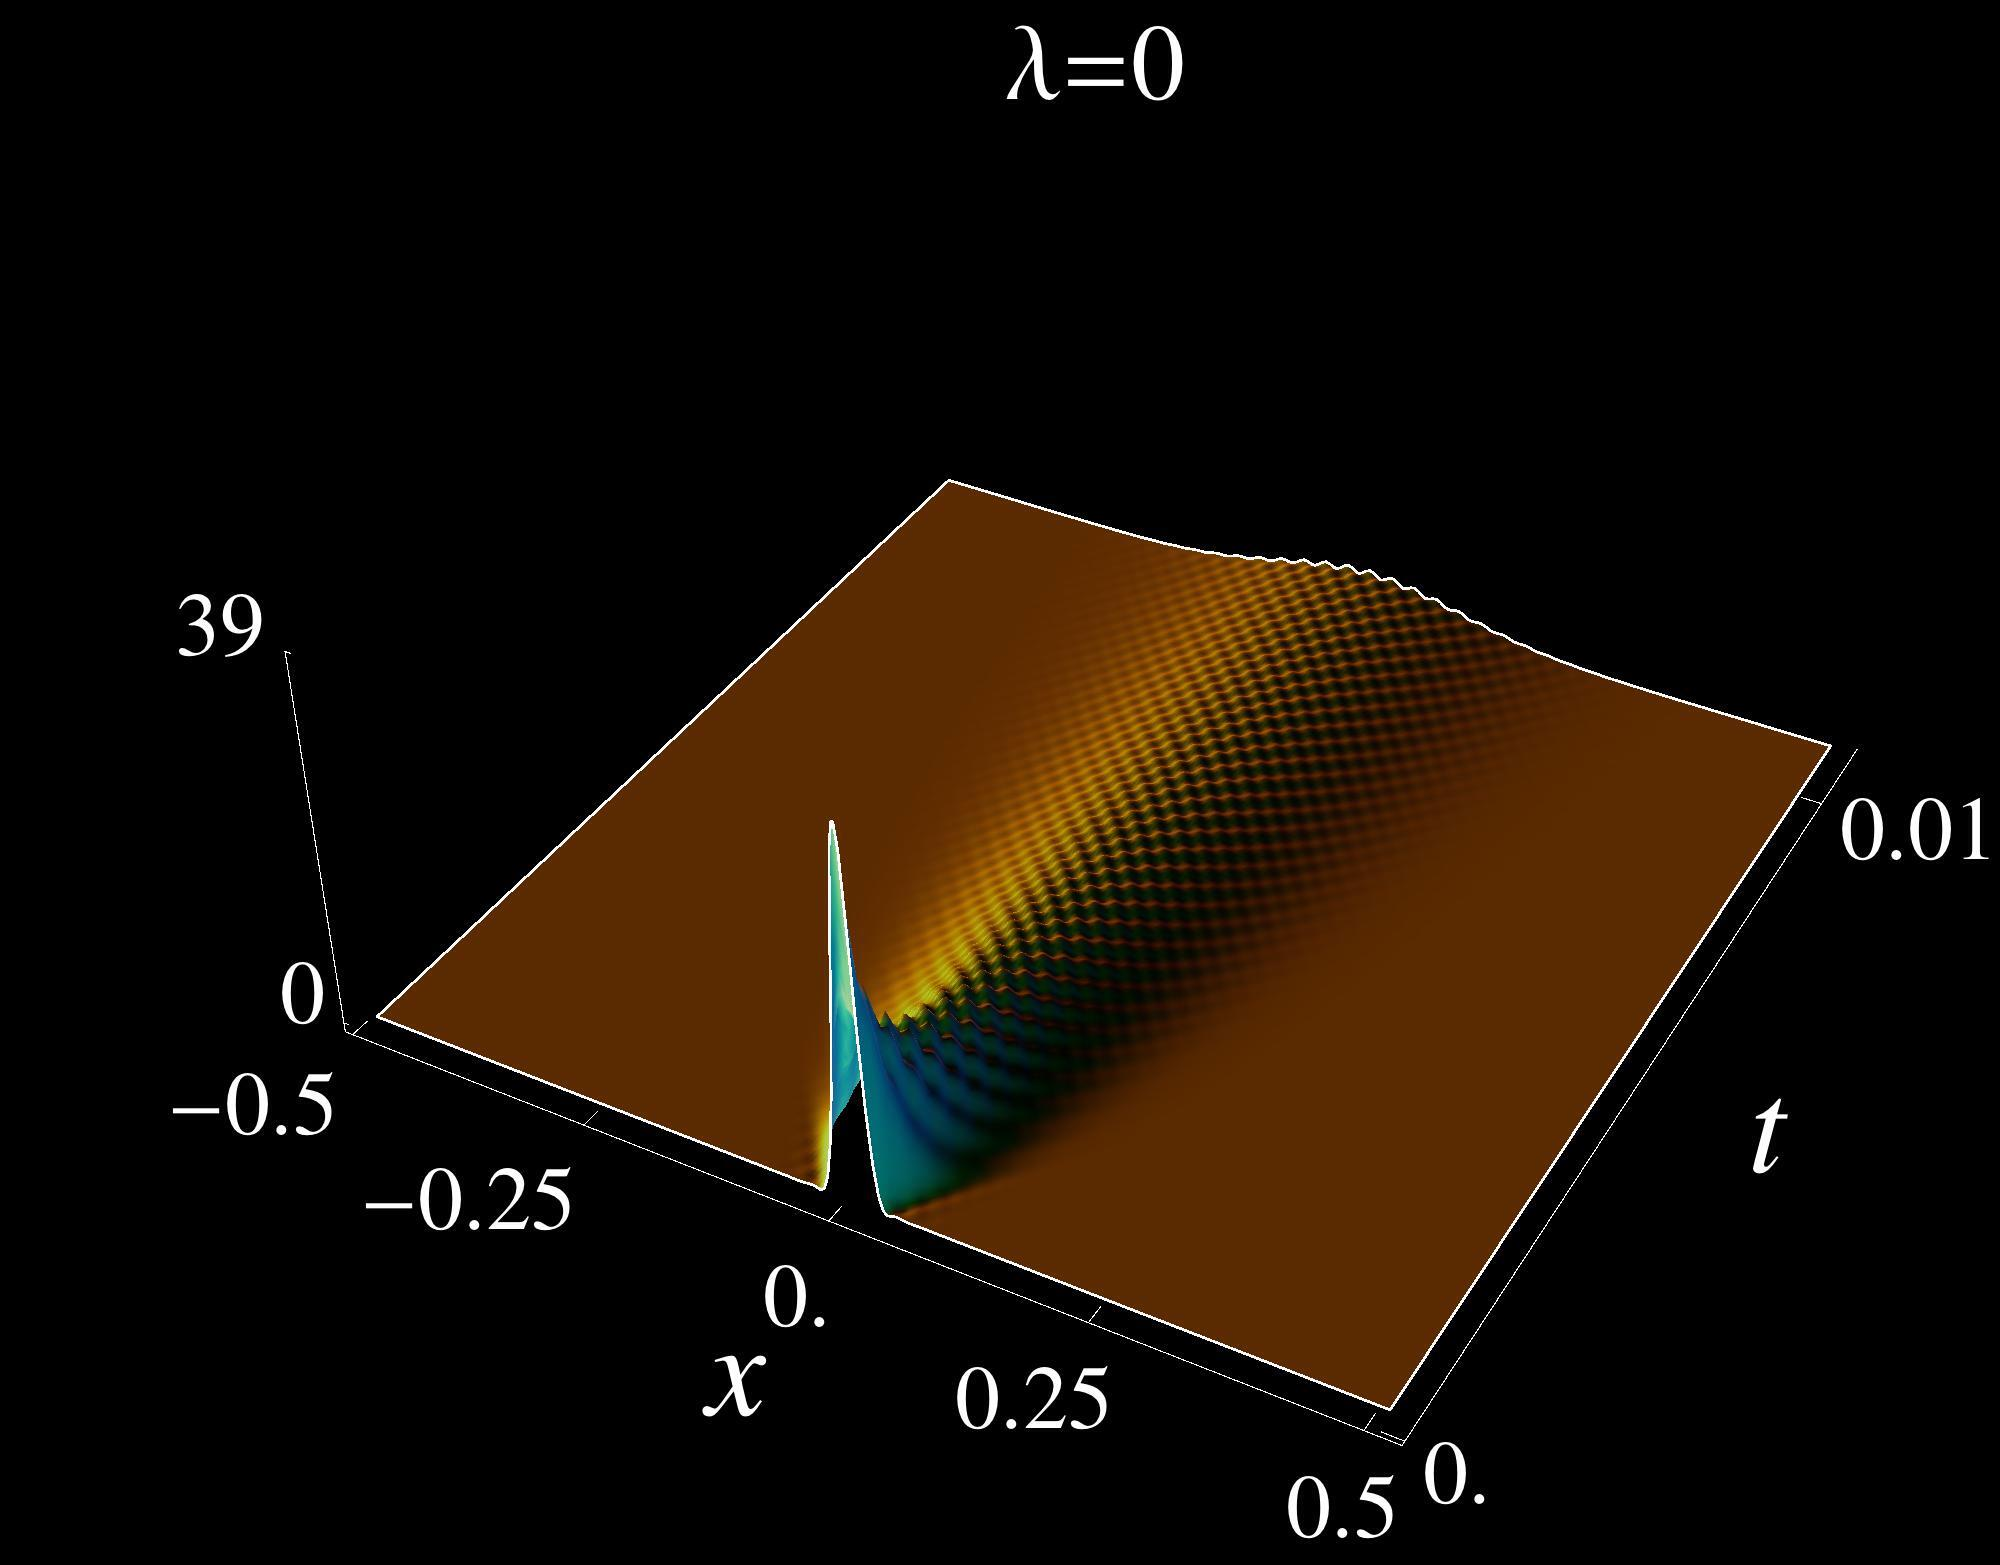
\includegraphics[scale=0.05]{figs/small_Delta_L0_cut-neg.jpeg}
    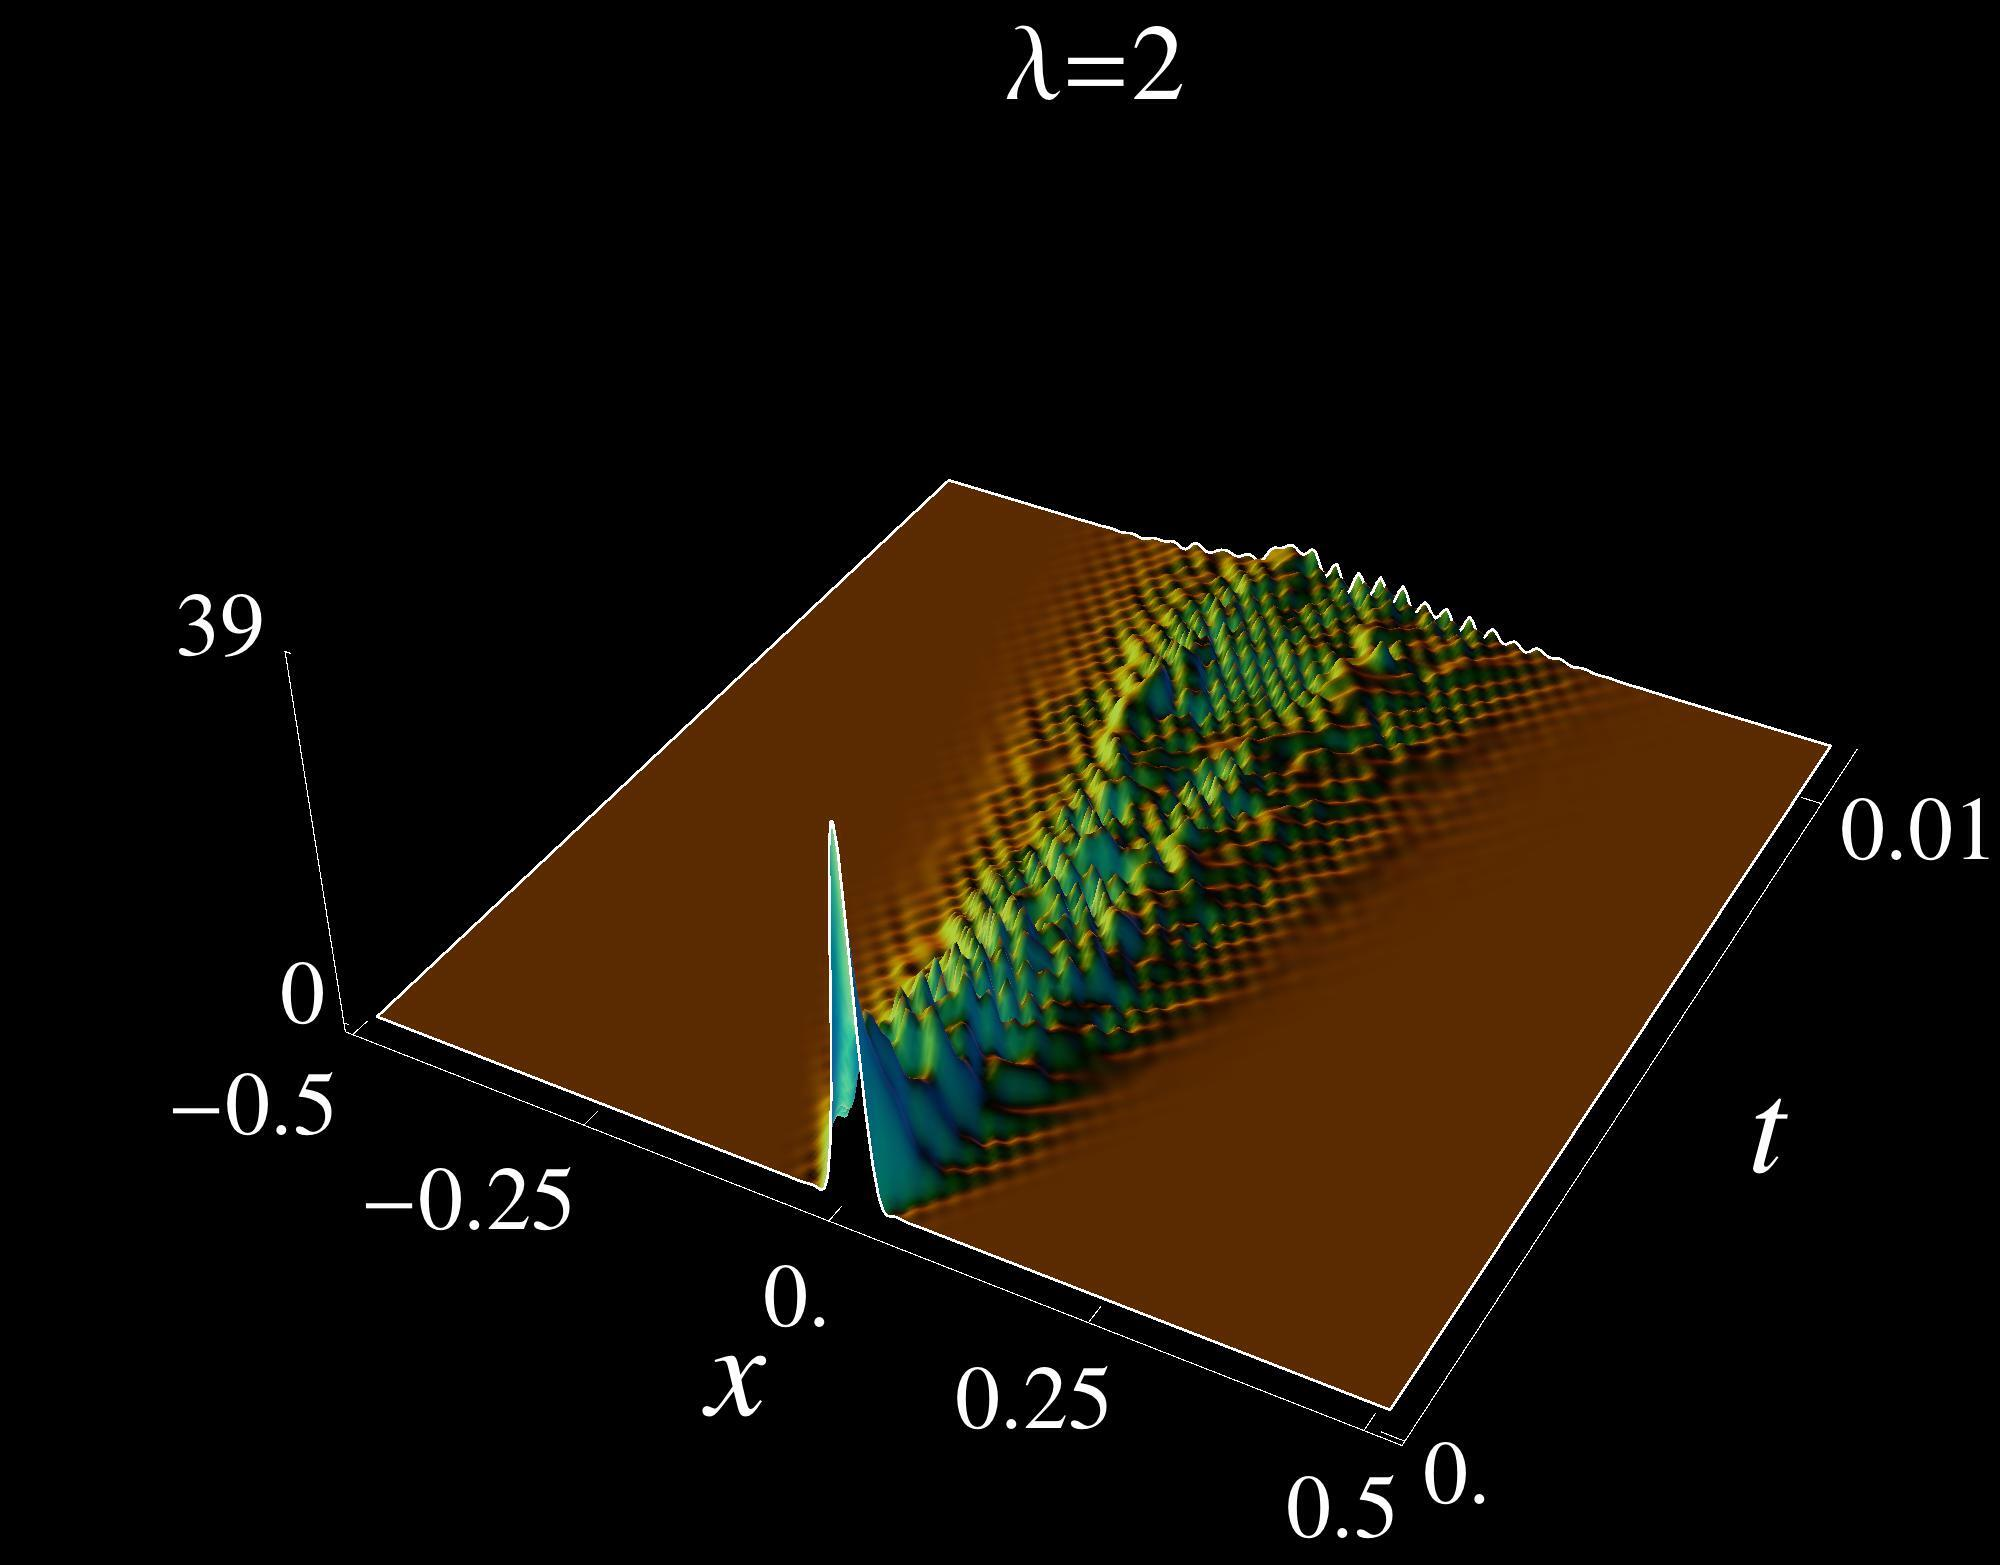
\includegraphics[scale=0.05]{figs/small_Delta_L2_cut-neg.jpeg}
    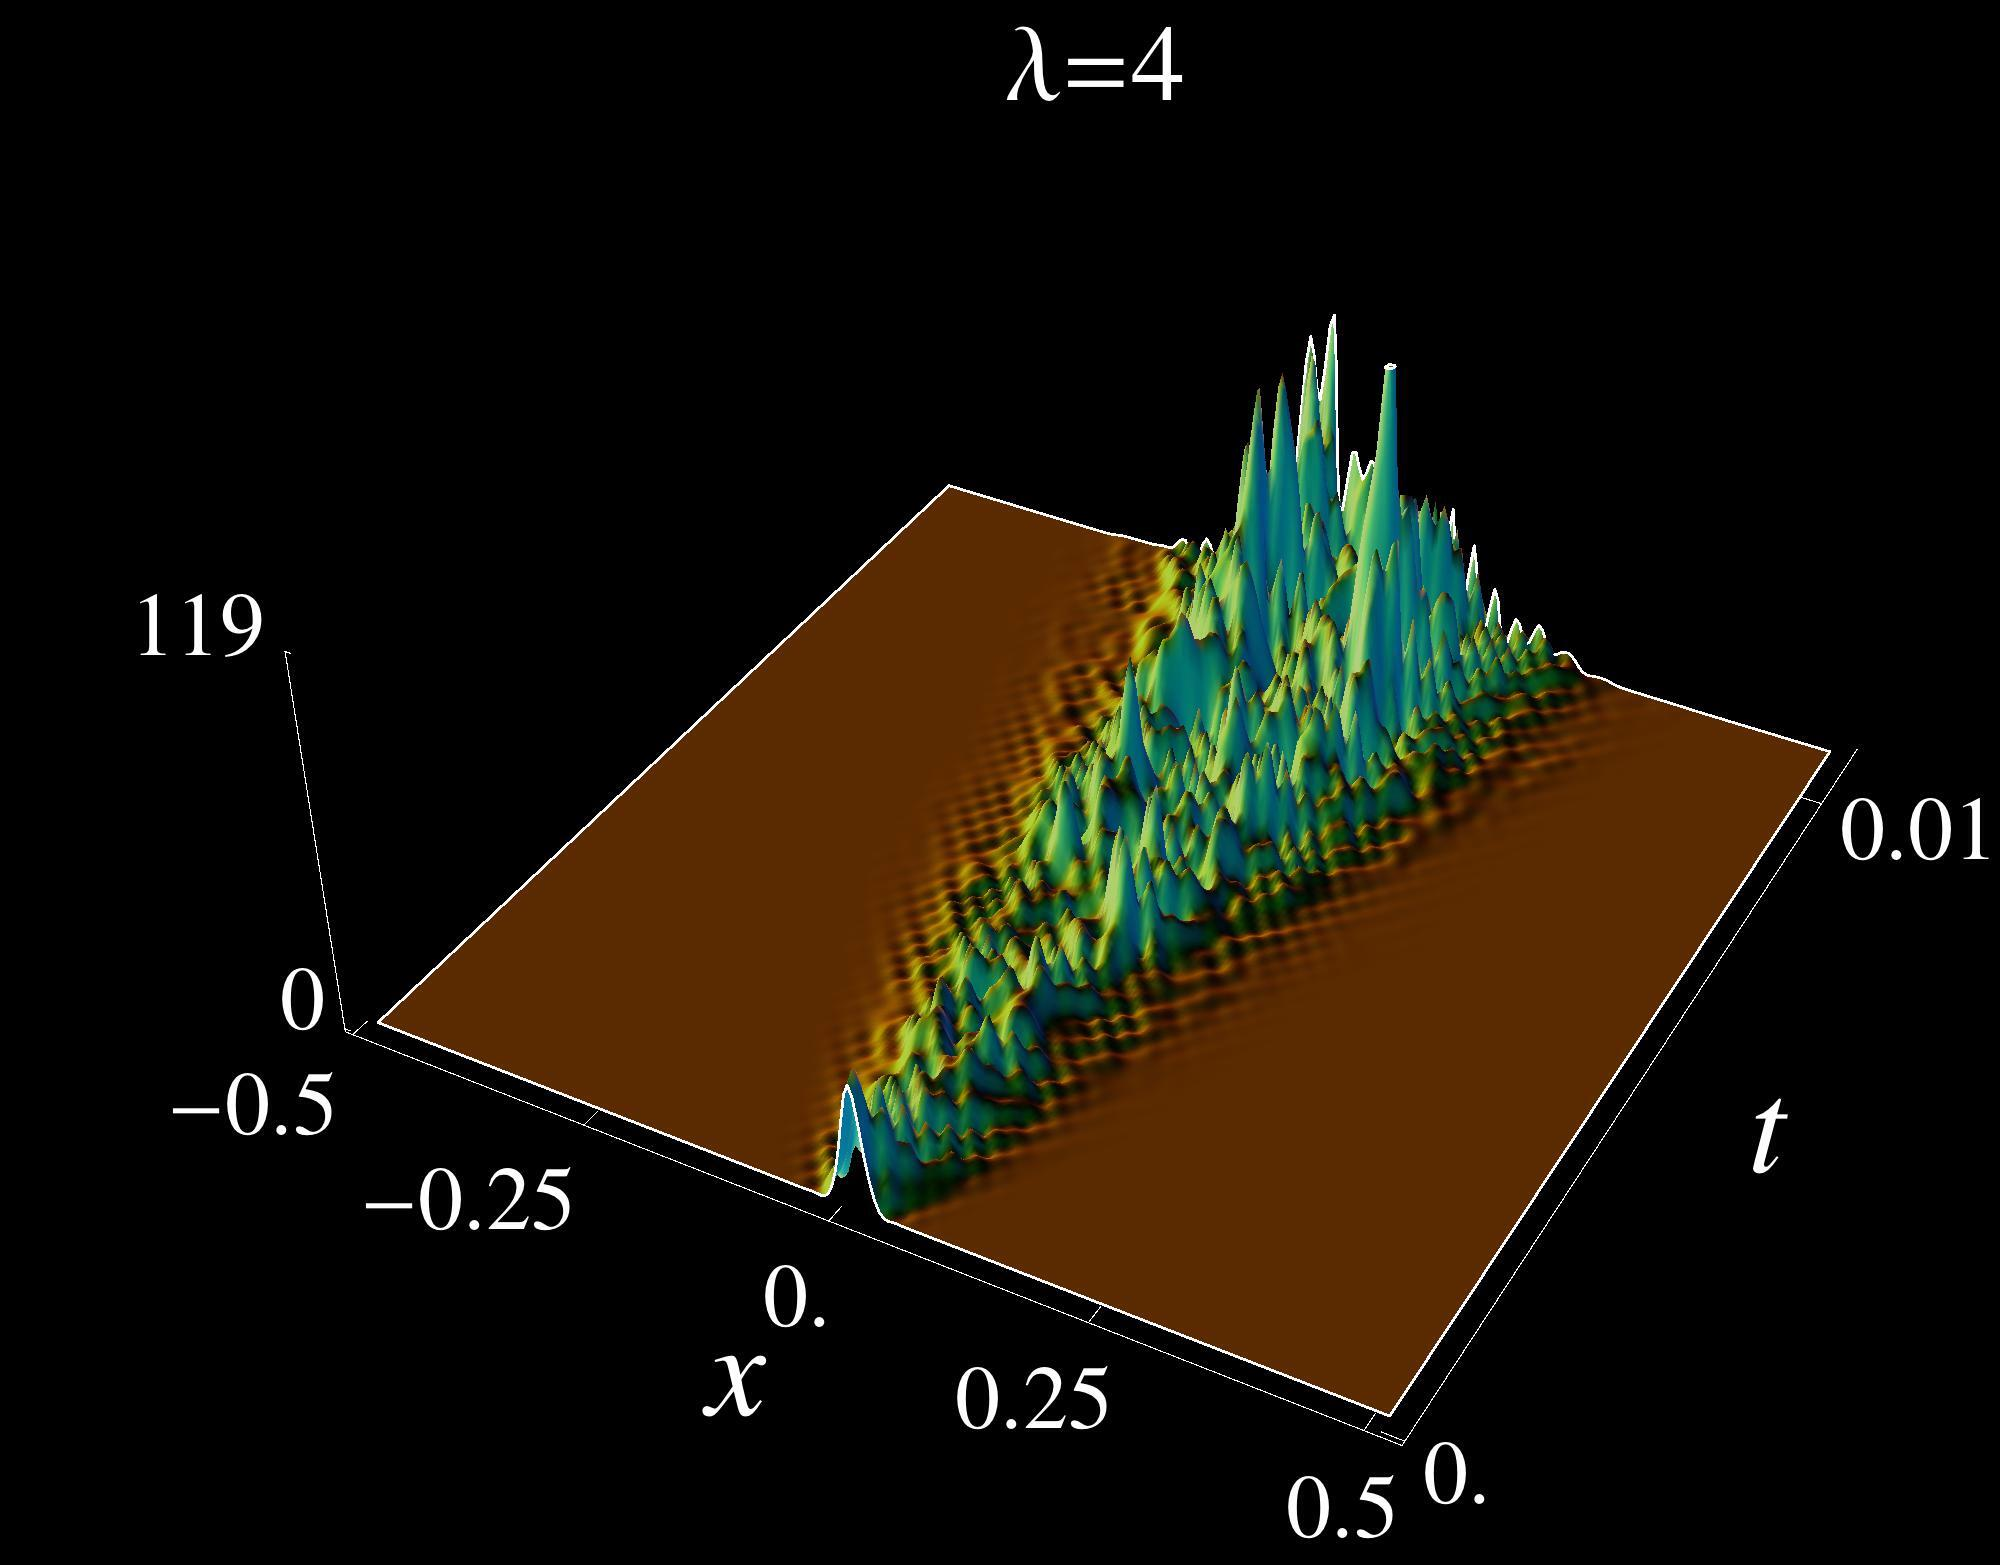
\includegraphics[scale=0.05]{figs/small_Delta_L4_cut-neg.jpeg}\\ \vfill
    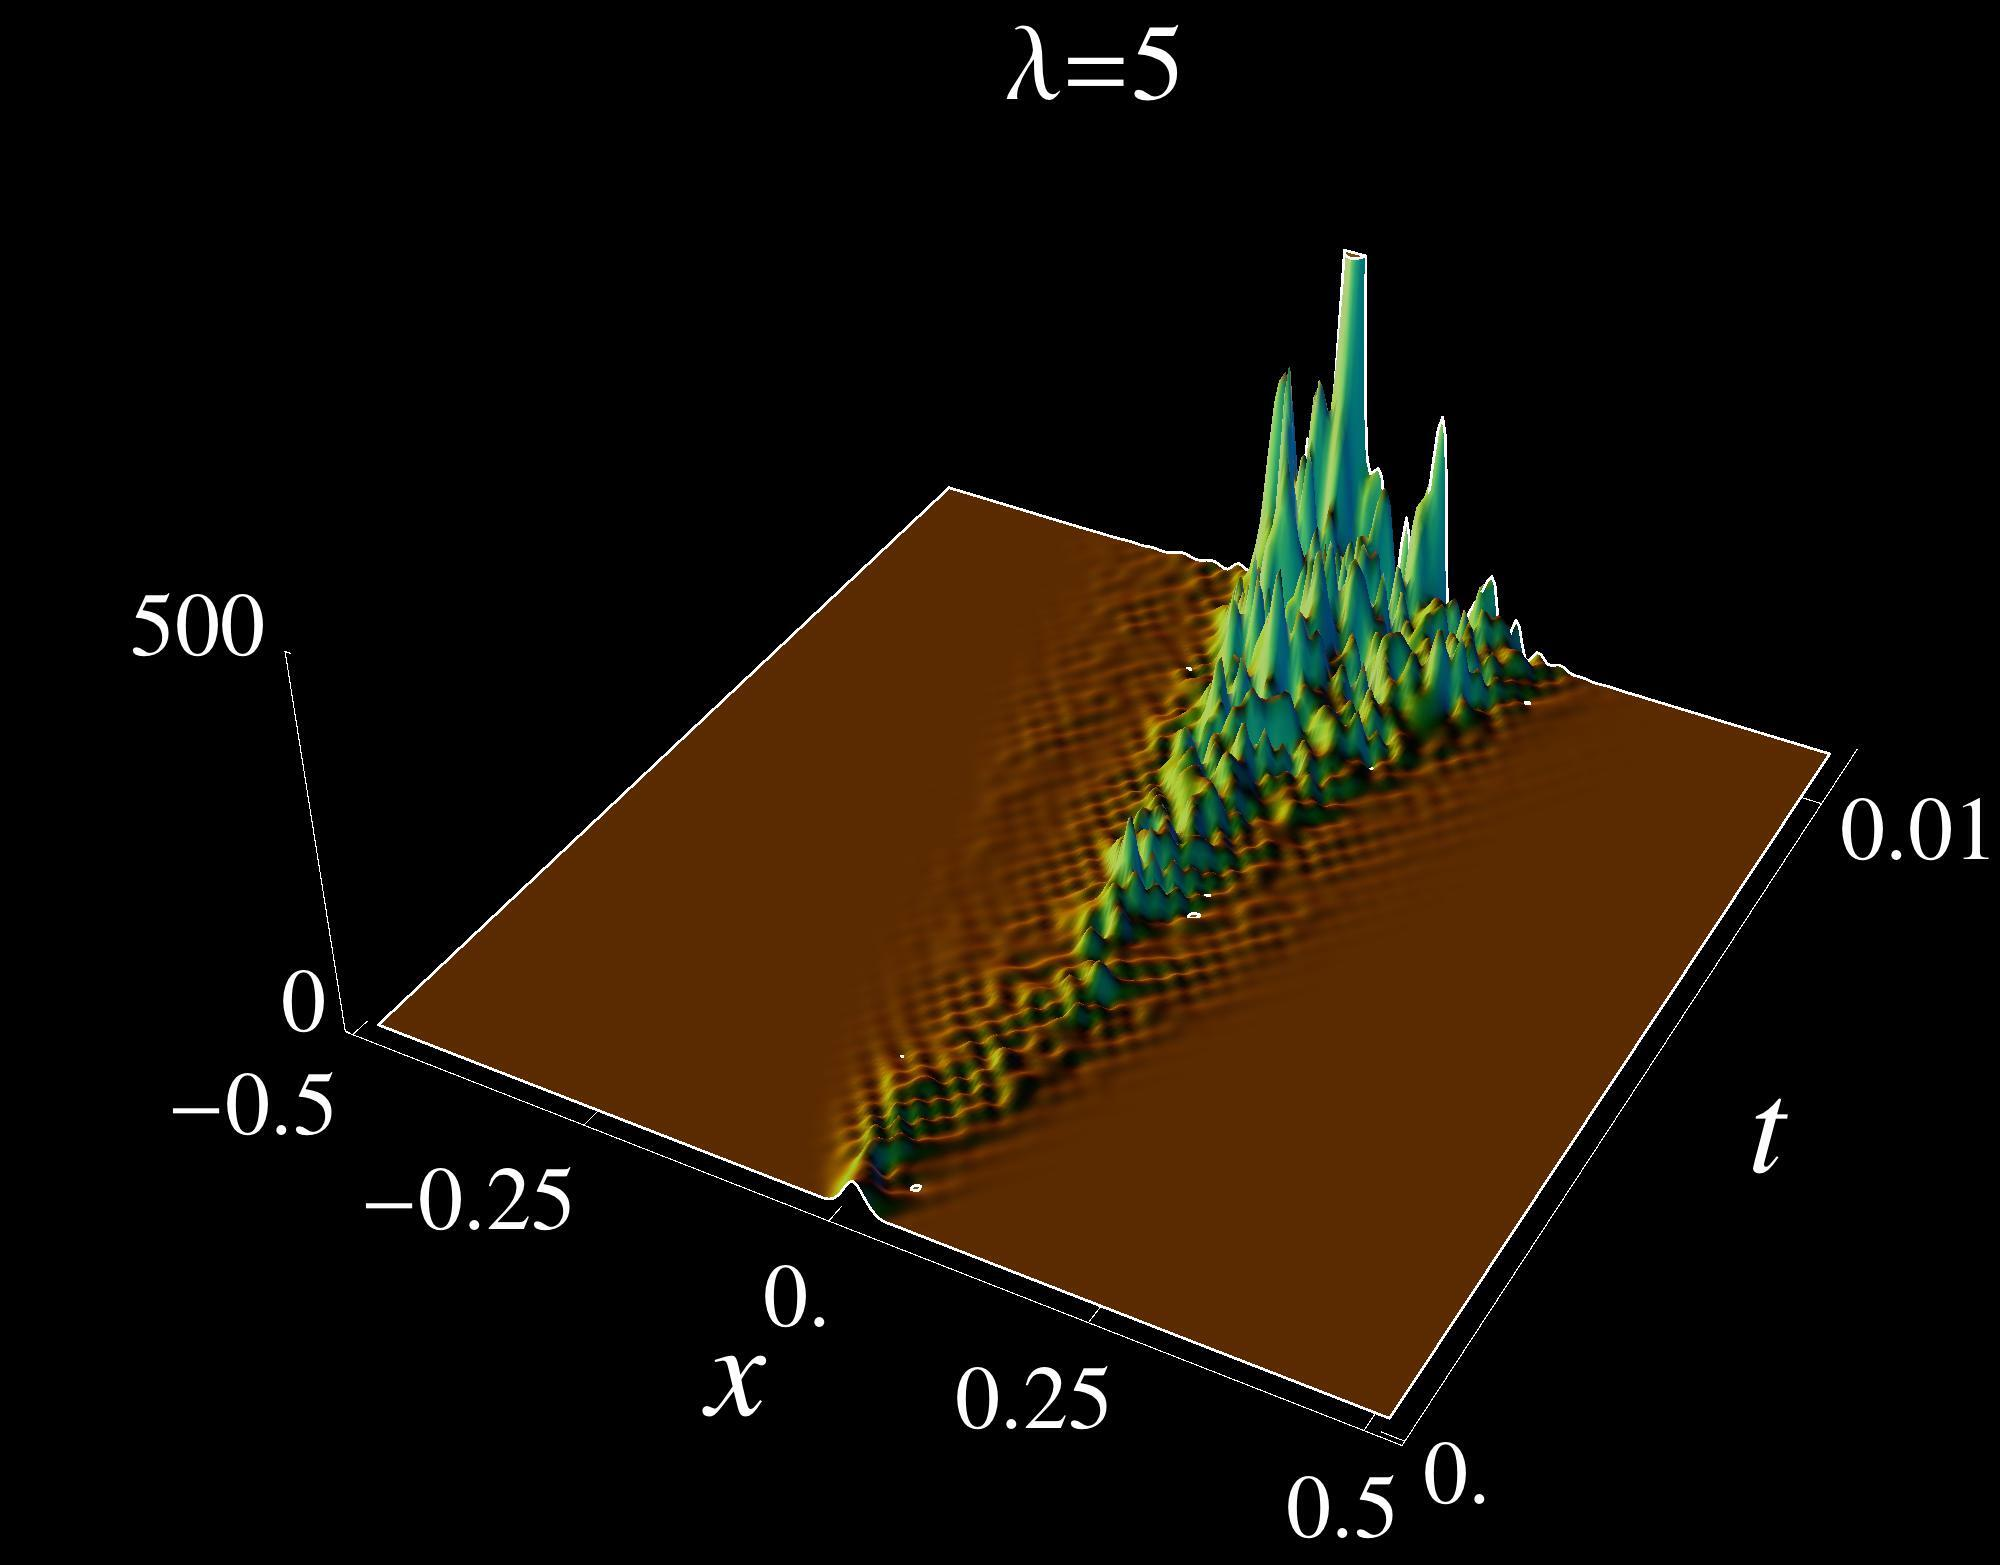
\includegraphics[scale=0.05]{figs/small_Delta_L5_cut-neg.jpeg}
    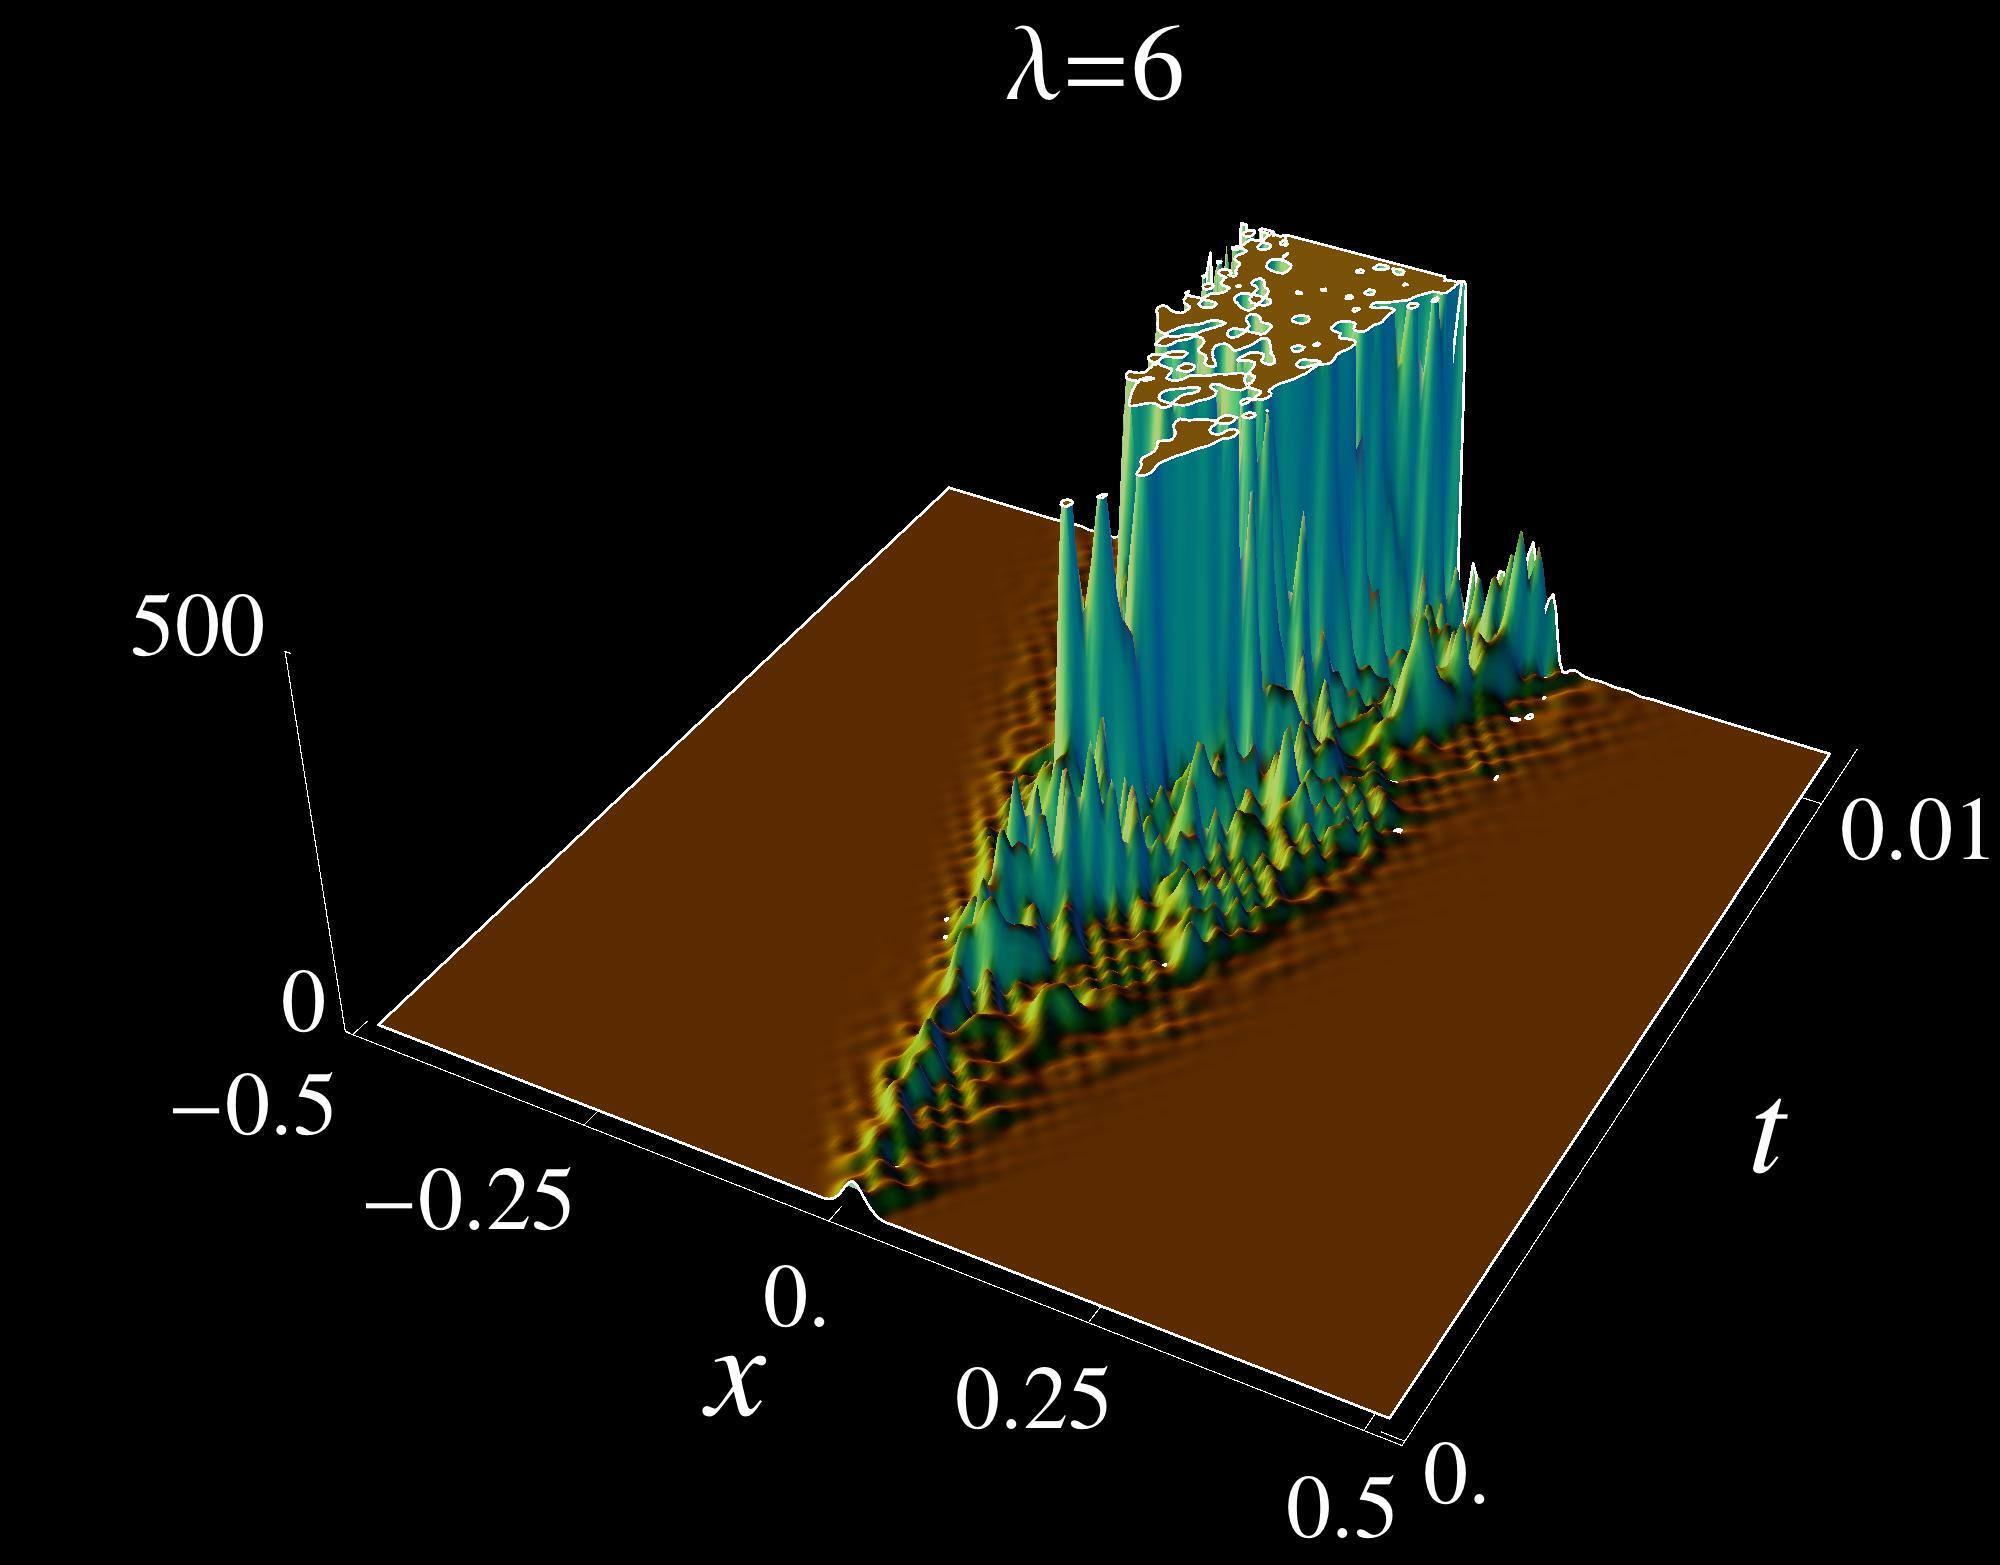
\includegraphics[scale=0.05]{figs/small_Delta_L6_cut-neg.jpeg}
    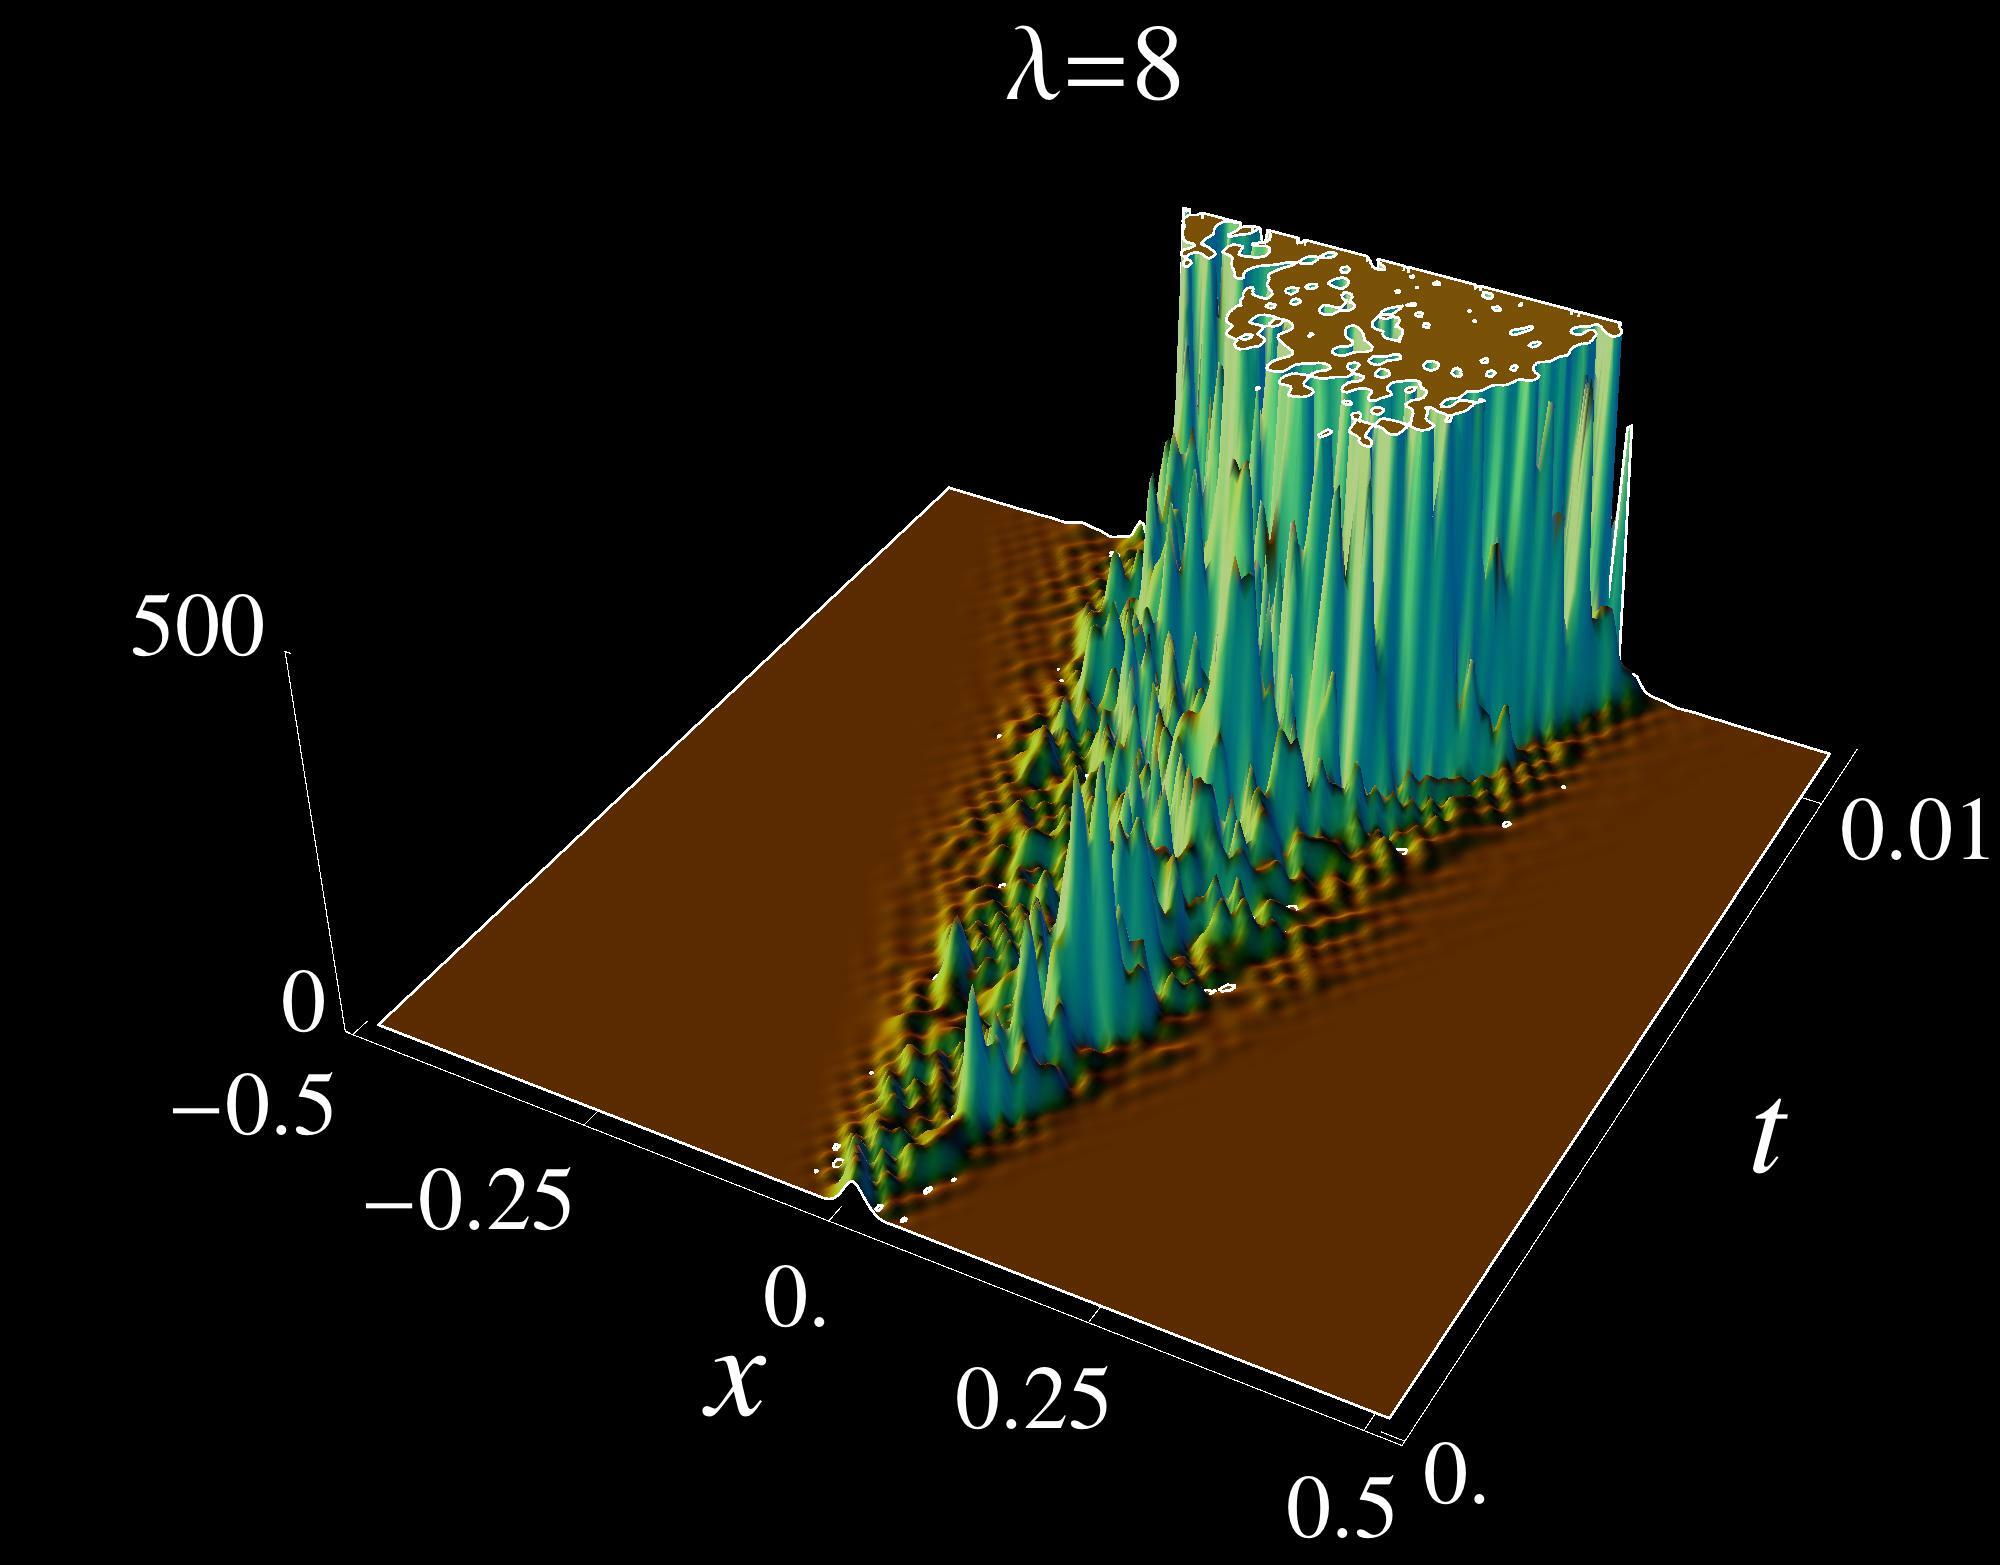
\includegraphics[scale=0.05]{figs/small_Delta_L8_cut-neg.jpeg}
    \only<8>{\phantom{aaa}\\[3.3em]
    \phantom{aaaaaa}}
    }
  \vfill
  \only<9>{
    \begin{center}
       The rate of the propagation of the tall peaks $\asymp \lambda^2$ \\[0.5em]
       {\footnotesize [L.C. \& Dalang, 15]}.
    \end{center}
    }
\end{frame}
% }}}
% {{{ 7.
\begin{frame}<5-6>{Various approaches for SPDE's}
\begin{itemize}
  \item -- Semigroup approach (Da Prato, et al). \hfill $u(t)\in L^p(\Omega,\calH)$\\[1em]
  \item[] -- Variational approach (R\"ockner, et al).\hfill Gel'fand triple\\
  %  \begin{itemize}
  %   \item[\Smiley{}] A generalization of finite dim. SDE to infinite dim. case.
  %   \item[] Cover more nonlinear eq.'s: stoch. Burger's eq., stoch. porous media eq.
  %   \item[] Existence, ergodicity, etc.
  %   \item[\Frowny{}] Not convenient for studying the spatial properties of the solution.
  %  \end{itemize}
  \vfill
  \item \alert<6>{Random field approach (Walsh, Dalang, et al.) \hfill $u(t,x)\in L^p(\Omega)$
    \only<5>{\\[1em]
    \hspace{6em} \phantom{The approach that we are using!}}
    \only<6>{\\[1em]
    \hspace{6em} The approach that we are using!}}
  \vfill
  \item -- Regularity structure (Hairer): \hfill Singular SPDEs\\[1em]
  \item[] -- Paracontrolled distributions (Gubinelli, et al)
  \pause
  %   \begin{itemize}
  %   \item[\Smiley{}] ``Singular SPDE'': the Kardar-Parisi-Zhang (KPZ) eq. \hfill(Interface propagation)
  %   \item[] \hspace{7.5em} $\Phi^4_3$ \hfill(quantum quantification model)
  %   \item[] \hspace{7.5em} PAM \hfill (critical dimension $d=2$, space white noise)
  %   \item[] Natural to obtain some pathwise properties.
  %   \item[\Frowny{}] Local theory. No probabilistic moments yet!
  %  \end{itemize}
\end{itemize}
\end{frame}
% }}}
% {{{ 8.
\begin{frame}[4-]{Stochastic Heat Equation on $\R^d$}
  \begin{align}\tag{SHE}
    \label{E:FracHt}
    \hspace{-1em}
     \begin{cases}
        \left(\displaystyle\frac{\partial}{\partial t} -\frac{1}{2}\Delta \right) u(t,x) = \rho(u(t,x))  \dot{W}(t,x),& t>0\;,\: x\in\R^d\\[0.5em]
        u(0,\cdot) = \mu(\cdot)
     \end{cases}
  \end{align}
  \vfill
  \begin{enumerate}
    \item $\rho$ is globally Lipschitz continuous s.t. $\rho(0)=0$.\\[1em]
    \item $\mu$ is {\it rough} (measure+integrability condition).\\[1em]
    \item $\W$ is white in time and colored in space ($f$ nonneg. \& nonneg. definite):
      \[
        \E\left[\W(t,x)\W(s,y)\right] = \delta_0(t-s)f(x-y)
      \]
    \vfill
    \item $\rho(u) = \lambda u$: {\it Parabolic Anderson Model}.
  \end{enumerate}
\end{frame}
% }}}
% {{{ 9.
\begin{frame}{Mild solution}
\begin{itemize}
  \item[]
  \vspace{0.5em}
    \[
      u(t,x) = J_0(t,x) +\underbrace{\mystrut{1.3em}\int_0^t\int_{\R^d} G(t-s,x-y)\rho(u(s,y))W(\ud s\ud y)}_{\displaystyle =:I(t,x)}
    \]
  \vspace{3em}
  \item[$\dagger$] $\displaystyle G(t,x)=(2\pi t)^{-d/2}\exp\left(-\frac{|x|^2}{2t}\right)$
  \vspace{1em}
  \item[$\dagger$] $\displaystyle J_0(t,x) = \int_{\R^d}G(t,x-y)\mu(\ud y)$
\end{itemize}
\end{frame}
% }}}
\section{Comparison principles: Overview}
% {{{ 11.
\begin{frame}{Comparison principles for SHE}
  \begin{align}\tag{SHE}
    \label{E:FracHt}
    \hspace{-1em}
    \begin{cases}
      \left(\displaystyle\frac{\partial}{\partial t} -\frac{1}{2}\Delta \right) u(t,x) = \rho(u(t,x))  \dot{W}(t,x),& t>0\;,\: x\in\R^d\\[0.5em]
      u(0,\cdot) = \mu(\cdot)
    \end{cases}
  \end{align}
  \vfill
  \begin{itemize}
    \item[Let]  $u_1$ and $u_2$ be two solutions to (SHE) obtained either by
    \[
      \mu     \rightarrow \mu_1,\mu_2         \quad\text{or}\quad
      \rho    \rightarrow \rho_1,\rho_2       \quad\text{or}\quad
      \dot{W} \rightarrow \dot{W}_1,\dot{W}_2 .
    \]
    \vfill
    \item[Question]  Can we compare $u_1$ \& $u_2$?\\[1em]
    In which sense?\\[1em]
    Why is it important?
  \end{itemize}
\end{frame}
% }}}
% {{{ 12.
\begin{frame}[label=current]
\begin{center}
  \def\a{6}
  \scalebox{0.9}{
  \begin{tabular}{ c | c }
    %   \hline
                                                 & \only<\a>{\cellcolor{darkpurple}}\\
    Sample-path comparison                       & \only<\a>{\cellcolor{darkpurple}}Stochastic (moment) comparison\\ \pause
                                                 & \only<\a>{\cellcolor{darkpurple}}\\ \hline
                                                 & \only<\a>{\cellcolor{darkpurple}}\\
    $\mu_1>\mu_2$                                & \only<\a>{\cellcolor{darkpurple}}$\rho_1(\cdot)\ge \rho_2(\cdot)$ \quad or \quad $f_1\ge f_2$\\[1em] \pause
    $\big\Downarrow$                             & \only<\a>{\cellcolor{darkpurple}}$\big\Downarrow$\\[1em]$
    u_1(t,x)>u_2(t,x)$\quad $\forall (t,x)$ a.s. & \only<\a>{\cellcolor{darkpurple}}$\E(u_1(t,x)^k)\ge \E(u_2(t,x)^k)$ \quad $\forall (t,x) ,k\ge 1$ \\[1em] \hline
                                                 & \only<\a>{\cellcolor{darkpurple}}\\ \pause
    Strict positivity $\sim$ Hopf-Cole Sol.      & \only<\a>{\cellcolor{darkpurple}}No Feynman-Kac formulas for nonlinear $\rho$\\[0.5em]
    Neg. moments $\sim$ Smooth density           & \only<\a>{\cellcolor{darkpurple}}Moment growth in $k\: \sim\:$ intermittency\\ \pause
                                                 & \only<\a>{\cellcolor{darkpurple}}\\ \hline
                                                 & \only<\a>{\cellcolor{darkpurple}}\\
    \small Mueller '91, Shiga '94                & \only<\a>{\cellcolor{darkpurple}}\small Joseph, Khoshnevisan \& \small Mueller '17\\
    \small Tessitore \& Zabczyk '98              & \only<\a>{\cellcolor{darkpurple}}\small Foondun, Joseph \& Li '18\\
    \small L.C. \& Kim '15, L.C. \& Huang '18    & \only<\a>{\cellcolor{darkpurple}}\small L.C. \& Kim '20 \\[1em]
  \end{tabular}
  }
 \end{center}
\end{frame}
% }}}
\section{\hspace{1em} {\it Stochastic}  comparison principles}
% {{{ 14.
\begin{frame}{Examples of stochastic comparisons}
\begin{itemize}
  \item[Assume~]  $\mu_1=\mu_2$ and $\dot{W}_1=\W_2$ but $\rho$'s are different:
    \[
      \text{either}\quad
      \rho_1(x)\le \rho_2(x)\le 0
      \quad\text{and}\quad \rho_1(x)\ge \rho_2(x)\ge 0\quad \text{for all $x\ge 0$,}
    \]
    % \vspace{0.3em}
  \begin{center}
   or
  \end{center}
  \vspace{0.3em}
  \item[Assume~] $\mu_1=\mu_2$ and $\rho_1=\rho_2$, but $\W$'s are different: $f_1\ge f_2$.
    \vfill
    \item[Eg. 1~] \textcolor{yellow!75!black}{\it Moment comparison principle}:
    $\forall m\in\bbN$, $\forall (t_\ell,x_\ell)\in (0,\infty)\times\R^d$, $\forall k_\ell\in\bbN$, $\ell=1,\cdots,m$,
    % For $m$ arbitrary space-time points $(t_\ell,x_\ell)\in (0,\infty)\times\R^d$ (not necessarily to be distinct) and $m$ integers $k_\ell\in\bbN$, $\ell=1,\cdots,m$, it holds that
     \begin{align*}
     \E\left[\prod_{\ell=1}^m u_1^{k_\ell}(t_\ell,x_\ell)\right]
     \ge
     \E\left[\prod_{\ell=1}^m u_2^{k_\ell}(t_\ell,x_\ell)\right].
    \end{align*}
    \\[1.5em]
  \item[] (This is the content in {\small [Joseph, et al '17] and [Foondun, et al '18]})
\end{itemize}
\end{frame}
% }}}
% {{{ 15.
\begin{frame}
\begin{itemize}
  \item[Eg. 2~]
    $\forall m\in\bbN$, $\forall (t_\ell,x_\ell)\in (0,\infty)\times\R^d$, $\forall k_\ell\in\bbN$, $\ell=1,\cdots,m$,
    \begin{align}\tag{$\star$}
      \E\left[\prod_{\ell=1}^m g_\ell^{k_\ell}(u_1(t_\ell,x_\ell))\right] \ge
      \E\left[\prod_{\ell=1}^m g_\ell^{k_\ell}(u_2(t_\ell,x_\ell))\right],
    \end{align}
    where $g_\ell(z)$ can be either
    \[
    x^{b_\ell}[\log(c_\ell+ x)]^{a_\ell}
    \quad\text{or} \quad x^{d_\ell},
    \]
    with $a_\ell, b_\ell,d_\ell\ge  1$ and $c_\ell \ge e$.
    \vfill
  \item[Eg. 3~] Statement in ($\star$) is true with $g_\ell(z)$ being either
    \[
      \exp\left(-\lambda_\ell z\right),\quad \frac{1}{(1+z)^{c_\ell}},\quad\text{or}\quad \log\left(\frac{z+a_\ell}{z+b_\ell}\right)
    \]
    with $\lambda_\ell>0$, $a_\ell>b_\ell>0$ and $c_\ell\ge 1$.
\end{itemize}
\end{frame}
% }}}
% {{{ 16.
\begin{frame}
\begin{itemize}
    \item[Eg. 4~] $\forall m\ge 1$, $t_m>\cdots >t_1>0$,  $k_1,\cdots k_m\in\bbN\setminus\{0\}$, $\alpha_1,\cdots,\alpha_m\in [2,\infty)$, and $x_{j}^\ell\in\R^d$ with $\ell=1,\cdots,m$ and $j=1,\cdots,k_\ell$ s.t.  $\left\{x_{k_1}^\ell,\cdots,x_{k_\ell}^\ell\right\}$ are distinct points for each $\ell$, \\
      \begin{multline*}
        \E\left(
        \prod_{\ell=1}^m \left[u_1^2\left(t_\ell,x_{1}^\ell\right)+\cdots+ u_1^2\left(t_\ell,x_{k_\ell}^\ell\right)\right]^{\frac{\alpha_\ell}{2}}
        \right)\\
        \ge
        \E\left(
        \prod_{\ell=1}^m \left[u_2^2\left(t_\ell,x_{1}^\ell \right)+ \cdots+u_2^2\left(t_\ell,x_{k_\ell}^\ell \right)\right]^{\frac{\alpha_\ell}{2}}
        \right).
      \end{multline*}
\end{itemize}
\end{frame}
% }}}
% {{{ 17.
\begin{frame}
\begin{itemize}
  \item[Eg. 5~] $\forall (t,x)\in(0,\infty)\times\R^d$, $c> 0$ and any integer $n\ge 1$, it holds that\\
    \begin{align}\tag{$\star$}
      \E\left(\left[u_1(t,x)-c\right]^{2n}\right) \ge
      \E\left(\left[u_2(t,x)-c\right]^{2n}\right).
    \end{align}
    \vspace{0.5em}
  \item[] In particular, by choosing $c=(\mu * G(t,\cdot))(x)$, ($\star$) tells us that all \textcolor{yellow!75!black}{\it centered moments} of even orders can be compared, i.e.,
  \vspace{0.5em}
    \[
      \E\left(I_1(t,x)^{2n}\right) \ge
      \E\left(I_2(t,x)^{2n}\right).
    \]
    % \item[] {\small When $n=1$, this is a comparison result for the variances. Only the comparison of variances (i.e., $n=1$) can be derived from the moment comparison principle, not for $n\ge 2$.}
    \vspace{2.5em}\\
    \noindent\textcolor{gray}{\rule{4cm}{0.6pt}}
    \begin{minipage}{0.7\textwidth}
      \footnotesize
      $\dagger$ Recall: $u_\ell(t,x) = J_0(t,x) +I_\ell(t,x)$, $\ell = 1,2.$
    \end{minipage}
\end{itemize}
\end{frame}
% }}}
% {{{ 18.
\begin{frame}
\begin{enumerate}
  \item[Eg. 6~] \textcolor{yellow!75!black}{\it (Slepian's inequality for SPDEs)} \\[0.5em]
    If $\mu_1=\mu_2$ and $\rho_1=\rho_2$, and if $f_1\ge f_2$ but $f_1$ and $f_2$ are {\it equal} to each other near the origin, then for all $a>0$, $t>0$, and $x_1,\cdots, x_N\in\R^d$, \\[1em]
    \[
    \bbP \left\{ \max_{1\leq k \leq N} u_1(t, x_k) \leq a  \right\} \geq \bbP \left\{ \max_{1\leq k \leq N} u_2(t, x_k) \leq a  \right\}.
    \]
    \vspace{2em}

    Formally, this is equivalent to take $g(x) = \one_{[0,a]}(x)$.
\end{enumerate}
\end{frame}
% }}}
% {{{ 19.
\begin{frame}{Difficulties  and hence contributions}
\begin{enumerate}
  \item \textcolor{yellow!75!black}{Dalang's condition} --- Weakest assumption for the correlation measure to have $L^2(\Omega)$ solution:
    \begin{align}
      \int_{\R^d}\frac{\widehat{f}(\ud \xi)}{1+|\xi|^2}<\infty. \tag{DL}
    \end{align}
    \vfill
  \item \textcolor{yellow!75!black}{Rough initial data}: $\mu$ is a (nonnegative) measure s.t.
    \[
      J_0(t,x)<\infty\quad \forall t>0,\:x\in\R^d
      \pause\qquad\Longleftrightarrow\quad
      \int_{\R^d}e^{-a|x|^2}\mu(\ud x)<\infty,\forall a>0.
    \]\pause
  \item[] E.g., \quad $\mu=\delta_0$, \quad $\mu(\ud x) = e^{+|x|^{3/2}}\ud x$, \quad $\mu(\ud x) = |x|^{-\beta}\ud x\: (\beta\in (0,d))$, \dots
    \vfill
  \item \textcolor{yellow!75!black}{Stochastic comparison}: goes beyond the moment comparison and covers, e.g., Examples 2--6.
\end{enumerate}
\end{frame}
% }}}
% {{{ 20.
\begin{frame}{Multiple-time comparison over certain function sets $\bbF$}
\begin{enumerate}
  \item[Def.~] Let $\{u_i(t,x); (t,x)\in \R_+\times K\}$, $i=1,2$, be two random fields, where $K$ is the spatial index set.
  \item[] For some function cone $\bbF$, and some $n\ge 1$, we say that $u_1$ and $u_2$ satisfy
    \vspace{0.5em}
    \begin{center}
      the \textcolor{yellow!75!black}{\it multiple/$n$-time stochastic comparison principle \\over $\bbF$ with $u_1$ dominating $u_2$}
    \end{center}
    \vspace{1em}
    if for any $0<t_1<\cdots<t_n<\infty$, and $F_1,\dots, F_n\in\bbF$,
    it holds that\\[0.5em]
    \begin{align*}
      \E\left[\prod_{\ell=1}^n F_\ell\left(u_1(t_\ell,\cdot)\right)\right] \ge
      \E\left[\prod_{\ell=1}^n F_\ell\left(u_2(t_\ell,\cdot)\right)\right].
    \end{align*}
\end{enumerate}
\end{frame}
% }}}
% {{{ 21. Statement of Main Theorem
\begin{frame}[label=current]{Statement of main results}

  {\noindent\bf \underline{Theorem.}} (L.C. \& Kim '20)~
  Under Dalang's condition, for rough initial data,
  \begin{gather*}
    \text{if} \quad \rho_1(\cdot)\ge \rho_2(\cdot)\ge 0\quad\text{or}\quad\text{if}\quad f_1\ge f_2,
  \end{gather*}
  then for $K=\R^d$, $u_1$ and $u_2$ satisfy  \pause
  \vspace{1em}
  \begin{enumerate}
    \item the multiple-time stochastic comparison principle over $\bbF[C_{p,+}^{2,v}]$,
      \medskip
    \item the multiple-time stochastic comparison principle over $\bbF[C^{2,v}_{b,-}]$,
      \medskip
    \item the $1$-time stochastic comparison principle over $\bbF[C^{2,v}_p]$.
  \end{enumerate}
  \vfill
  \noindent\textcolor{gray}{\rule{4cm}{0.6pt}}\\[0.3em]
  \begin{minipage}{0.3\textwidth}
    \textcolor{gray}{
    \footnotesize
    $p$: \underline{polynomial growth}. \\
    $b$: \underline{bounded}.\\
    $v$: convex functions.}
  \end{minipage}
  \begin{minipage}{0.45\textwidth}
    \textcolor{gray}{
    \footnotesize
    $+$: first derivative nonnegative.\\
    $-$: first derivative nonpositive.\\
    \phantom{aaa}}
  \end{minipage}
\end{frame}
% }}}
% {{{ 22. Approximation diagram
\begin{frame}[fragile]{Proof strategy: approximations of SHE}
  \tikzset{
    invisible/.style={opacity=0},
    visible on/.style={alt={#1{}{invisible} }},
    alt/.code args={<#1>#2#3}{%
      \alt<#1>{\pgfkeysalso{#2}}{\pgfkeysalso{#3}} % \pgfkeysalso doesn't change the path
    },
  }
  \usetikzlibrary{shapes,arrows}
  \tikzstyle{decision} = [diamond, draw, fill=blue!20!black,  node distance=3cm,  text width=4.5em,   text badly centered, inner sep=0pt]
  \tikzstyle{block1} = [rectangle, draw, fill=blue!20!black,  node distance=12em, text centered,      rounded corners,     minimum height=4em]
  \tikzstyle{block2} = [rectangle, draw, fill=green!20!black, node distance=12em, text centered,      rounded corners,     minimum height=4em]
  \tikzstyle{cloud} = [ellipse,    draw, fill=red!20!black,   node distance=7em,  minimum height=2em, align=center]
  \tikzstyle{line} = [->,          draw, shorten <=0.3em,     shorten >=0.3em]
  \begin{tikzpicture}[node distance = 1em, auto]
    % Place nodes
    \node [tape, draw, text width=6em, text centered, visible on=<1->] (1) {$u(t,x)$ solves\\ (SHE)};

    \node [block1, text width=8em, below of=1, node distance=7em, visible on=<2->] (2) {Regularization\\ of initial data \\ \& noise $u_{\epsilon_1}(t,x)$};
    \path [line,visible on=<2->] (1) -- (2);

    \node [block1, text width=8em, right of=2,visible on=<3->] (3) {Mollification\\ of Laplace \\ $u_{\epsilon_1,\epsilon_2}(t,x)$};
    \path [line,visible on=<3->] (2) -- (3);


    \node [block1, text width=8em, right of=3, visible on =<4->] (4) {Discretization\\ in space \\ $u_{\epsilon_1,\epsilon_2}(t,[x]_\delta)$};
    \path [line,visible on =<4->] (3) -- (4);

    \node [block2, text width=8em, below of=4 ,node distance=7em, visible on =<5->] (5) {Interacting\\ diffusions on $\bbZ^d$\\ $U(t,i)$};
    \node[draw,dashed, rectangle, minimum height=13em, minimum width=11em,rounded corners,visible on =<5->] (0) at ($(4)!0.5!(5)$) {};


    \node [block2, text width=8em, left of=5, visible on =<6->] (6) {Truncating \& \\ mollifying $\rho$ \\ s.t. $\rho\in C_c^2(\R_+)$\\ $U_{\epsilon}(t,i)$};
    \path [line,visible on =<6->] (5) -- (6);

    \node [block2, text width=8em, left of=6,visible on =<7->] (7) {Truncating $\bbZ^d$ to\\ finite-dim. SDE \\ $U_{\epsilon,m}(t,i)$};
    \path [line,visible on =<7->] (6) -- (7);

    \node [cloud, below of=7,align=center,node distance=6em,visible on =<8->] (8) {\underline{Lemma 1}: Stoch.\\ comparisons};
    \path [line,>=stealth', double = black, double distance = 0.1em, visible on =<8->] (7) -- (8);

    \node [cloud, below of=5,align=center,node distance=6em,visible on =<9->] (9) {\underline{Lemma 2}: Stoch.\\ comparisons};
    \path [line,>=stealth', double = black, double distance = 0.1em, visible on =<9->] (5) -- (9);

    \node [cloud, right of=1,align=center,node distance=12em,visible on =<10->] (10) {\underline{Thm}: Stoch.\\ comparisons};
    \path [line,>=stealth', double = black, double distance = 0.1em, visible on =<10->] (1) -- (10);
  \end{tikzpicture}
\end{frame}
% }}}
% {{{ 23. Lemma 1.
\begin{frame}<1,2,4>
\[
  d U(t, i)=\kappa \sum_{j\in K} p_{i,j} \left( U(t, j)- U(t, i)\right) \ud t + \rho (U(t,i)) \ud M_i(t), \quad i\in K
\]
\vfill
{\noindent\bf \underline{Lemma 1}.} (L.C. \& Kim '20)~
For the finite (i.e., $|K|<\infty$) interacting diffusion eq.,
\begin{gather*}
  \text{if} \quad \rho_1(\cdot)\ge \rho_2(\cdot)\ge 0\quad\text{or}\quad\text{if}\quad \gamma_1\ge \gamma_2,
\end{gather*}
where $\rho_i\in C_c^2(\R_+)$,
then $u_1$ and $u_2$ satisfy all the comparison results in Theorem.

\vfill
\pause
Ideas of proof: Follows closely to {\small [Cox, et al '96]}: \\[1em]
\begin{center}
  \it Integration-by-parts formula \\[0.6em]
  Trotter's product formula \\[0.6em]
  Markov properties (for $n$-time case)
\end{center}
with necessary changes to make in order to take care of \pause
\begin{itemize}
 \item correlated noise and
 \item comparison over the correlation function $\gamma$'s.
\end{itemize}
\end{frame}
% }}}
% {{{ 24. Integration-by-parts formula
\begin{frame}<2->
\begin{itemize}
  \vfill
  \item[] Let $T_t^{(\ell)}$ be the semigroup, i.e., $T_t^{(\ell)} F(x):=\E_{x}\left[ F\left(U_\ell(t,\cdot)\right)\right]$ and $G_\ell$ be the corresponding infinitesimal generator, $\ell\in \{1,2\}$:
  \begin{align*}
    G^{(\ell)} = \kappa &\sum_{1\leq i, j \leq d} \left(p_{i,j}-\delta_{i,j}\right) z_j D_i +
    \begin{cases}
      \displaystyle \frac{1}{2}\sum_{1\leq i, j \leq d} \rho_\ell(x_i)\rho_\ell(x_j) \gamma(i-j) D_iD_j\\[1em]
      \displaystyle \frac{1}{2}\sum_{1\leq i, j \leq d} \rho(x_i)\rho(x_j) \gamma_\ell(i-j) D_iD_j
    \end{cases}
  \end{align*}
  \vfill
  \item \textcolor{yellow!75!black}{\bf Integration-by-parts formula}
    \[
      T_t^{(1)} - T_t^{(2)} = \int_0^t T_s^{(1)}\left[ G^{(1)} - G^{(2)} \right] T^{(2)}_{t-s} \,\, \ud s
    \]
    \vfill
  \item We only need to show that
    \begin{align*}
      D_iD_j & T_t F(z) \geq 0 \qquad \forall i, j, t, z.\\ \pause
             &||\\
      \underbrace{\left( D_iD_j F \right)}_{\ge 0} &\: \underbrace{TF_t(z)}_{\stackrel{?}{\ge} 0}
    \end{align*}
\end{itemize}
\end{frame}
% }}}
% {{{ 25. Trotter's product formula
\begin{frame}<4>
  \begin{eqnarray*}
    &G^{(\kappa,\rho)}&\\
    &||& \\
    \underbrace{\mystrut{1em} \kappa \sum_{1\leq i, j \leq d} \left(p_{i,j}-\delta_{i,j}\right) z_j D_i}_{\displaystyle:= G^{(\kappa,0)}}\quad &+& \quad
    \underbrace{\mystrut{1em} \displaystyle \frac{1}{2}\sum_{1\leq i, j \leq d} \rho(x_i)\rho(x_j) \gamma(i-j) D_iD_j }_{\displaystyle:= G^{(0,\rho)}}
  \end{eqnarray*}
  \begin{minipage}{0.4\textwidth}
    \begin{align*}
    \begin{cases}
      \displaystyle dU(t, i)=\rho\left(U(t, i) \right) d M_i(t)\\
      \displaystyle U(0,i) = u_0(i)
    \end{cases}
    \end{align*}
    \[\rotatebox[origin=c]{90}{$\sim$}\]
    \[T^{(\kappa,0)}\]
  \end{minipage}
  \hfill
  \begin{minipage}{0.5\textwidth}
    \begin{align*}
    \begin{cases}
      dU(t, i)=\kappa \sum_{j=1}^d (p_{i,j}-\delta_{i,j}) U(s,j) \ud t\\
      U(0,i) = u_0(i)
    \end{cases}
    \end{align*}
    \[\rotatebox[origin=c]{90}{$\sim$}\]
    \[T^{(0,\rho)}\]
  \end{minipage}
  \vfill
  \mySeparateLine
  \begin{center}
    \textcolor{yellow!75!black}{\bf Trotter's product formula}\\
    \begin{align*}
      \lim_{k\rightarrow\infty}\left[ T_{t/k}^{(\kappa,0)} T_{t/k}^{(0,\rho)}\right]^k=T_t^{(\kappa,\rho)}
    \end{align*}
  \end{center}
  \myEnd
\end{frame}
% }}}
% {{{ 26. Lemma 2.
\begin{frame}[label=current]
\[
  d U(t, i)=\kappa \sum_{j\in Z^d} p_{i,j} \left( U(t, j)- U(t, i)\right) \ud t + \rho (U(t,i)) \ud M_i(t), \quad i\in Z^d
\]
\vfill
{\noindent\bf \underline{Lemma 2}.} (L.C. \& Kim '20)~
For the infinite interacting diffusion eq.,
\begin{gather*}
  \text{if} \quad \rho_1(\cdot)\ge \rho_2(\cdot)\ge 0\quad\text{or}\quad\text{if}\quad \gamma_1\ge \gamma_2,
\end{gather*}
where $\rho_i\in \Lip$,
then $u_1$ and $u_2$ satisfy all the comparison results in Theorem.
\pause
\vfill
\begin{center}
  \renewcommand{\arraystretch}{1.8}
  \definecolor{LightCyan}{rgb}{0.88,1,1}
  \definecolor{Gray}{gray}{0.85}
  \begin{tabular}{ |c | c| c |c| }
  \hline
                     &  \thead{Cox, et al \\ PTRF '96}    &  \thead{Foondun, et al\\ AAP '18}                                                    &  \thead{L.C. \& Kim \\ EJP '20}\\ \hline \hline
  Noise              &  i.i.d. BM's                       &  \multicolumn{2}{c|}{\cellcolor{darkpurple} Correlated BM's } \\ \hline \hline
  Fun. Cones $\bbF$  &  $\bbF[C_{b}^{2,v}]$               &  \multicolumn{1}{c}{\tabularCenterstack{c}{$x^n$, $n\in\bbN$ \\(moment comparison)}}  &  \multicolumn{1}{|>{\columncolor{darkpurple}}c|}{\tabularCenterstack{c}{$\bbF[C_{p}^{2,v}]$;\\ Slepian’s ineq.}}\\ \hline
  Comparing          &  \multicolumn{2}{c|}{only $\rho$}  &  \cellcolor{darkpurple} both $\rho$ and $\gamma$\\
  \hline
  \end{tabular}
\end{center}
\end{frame}
% }}}
% {{{ 27.
\begin{frame}<4>[label=current]

{\noindent\bf \underline{Theorem}.} (L.C. \& Kim '20)~
Under Dalang's condition, for rough initial data,
\begin{gather*}
  \text{if} \quad \rho_1(\cdot)\ge \rho_2(\cdot)\ge 0\quad\text{or}\quad\text{if}\quad f_1\ge f_2,
\end{gather*}
then for $K=\R^d$, $u_1$ and $u_2$, solutions to (SHE), satisfy  \pause
\vspace{1em}
\begin{enumerate}
  \item the multiple-time stochastic comparison principle over $\bbF[C_{p,+}^{2,v}]$,
    \medskip
  \item the multiple-time stochastic comparison principle over $\bbF[C^{2,v}_{b,-}]$,
    \medskip
  \item the $1$-time stochastic comparison principle over $\bbF[C^{2,v}_p]$.
\end{enumerate}
\vfill
\noindent\textcolor{gray}{\rule{4cm}{0.6pt}}\\[0.3em]
\begin{minipage}{0.3\textwidth}
  \textcolor{gray}{
  \footnotesize
  $p$: \underline{polynomial growth}. \\
  $b$: \underline{bounded}.\\
  $v$: convex functions.}
\end{minipage}
\begin{minipage}{0.45\textwidth}
  \textcolor{gray}{
  \footnotesize
  $+$: first derivative nonnegative.\\
  $-$: first derivative nonpositive.\\
  \phantom{aaa}}
\end{minipage}
\end{frame}
% }}}
% {{{ 28.
\begin{frame}[label=current]
\begin{center}
  \renewcommand{\arraystretch}{1.8}
  \definecolor{LightCyan}{rgb}{0.88,1,1}
  \definecolor{Gray}{gray}{0.85}
  \setlength\doublerulesep{0.5em}
  \begin{tabular}{ |c | c| c |c| }
    \hline
    % arXiv:1912.05350
                                                                               &  \thead{Joseph, et al \\ AOP '17}  &  \thead{Foondun, et al\\ AAP '18}  &  \thead{L.C. \& Kim\\ EJP '20}\\ \hline \hline
    Equation                                                                   &  SHE on $\R$                       &  Frac. SHE on $\R^d$                &  \cellcolor{darkpurple} SHE on $\R^d$ \\ \hline
    Noise                                                                      &  $f=\delta_0$                      &  Riesz kernel                       &  \cellcolor{darkpurple} Dalang's Condition \\ \hline
    Initial data& $u_0(x)\equiv 1$                                             &  $u_0(x)\ge 0$ bounded             &  \cellcolor{darkpurple} Rough \\ \hline \hline
    \multicolumn{1}{|c|}{\tabularCenterstack{c}{Function\\ cones $\bbF$}}      &  \multicolumn{2}{c|}{$x^n$, $n\in\bbN$ (moment comparison)}& \multicolumn{1}{>{\columncolor{darkpurple}}c|}{\tabularCenterstack{c}{More general;\\ Slepian’s ineq.}}\\ \hline
    Comparing                                                                  &  \multicolumn{2}{c|}{only $\rho$}  &  \cellcolor{darkpurple} both $\rho$ and $\W$ \\ \hline\hline
    \multicolumn{1}{|c|}{\tabularCenterstack{c}{Mollification\\ of $\Delta$}}  &  \multicolumn{2}{c|}{Random walk}  &  \cellcolor{darkpurple} Yoshida approximation\\ \hline
  \end{tabular}
\end{center}
\end{frame}
% }}}
\section{ \hspace{1em} {\it Sample-path} comparison principles}
% {{{ 30.
\begin{frame}<6>[label=current]
\begin{center}
  \def\a{6}
  \scalebox{0.9}{
  \begin{tabular}{ c | c }
  %   \hline
  \only<\a>{\cellcolor{darkpurple}}                                                &                                                                  \\
  Sample-path comparison  \only<\a>{\cellcolor{darkpurple}}                        & Stochastic (moment) comparison                                   \\ \pause
  \only<\a>{\cellcolor{darkpurple}}                                                &                                                                  \\ \hline
  \only<\a>{\cellcolor{darkpurple}}                                                &                                                                  \\
  $\mu_1>\mu_2$  \only<\a>{\cellcolor{darkpurple}}                                 & $\rho_1(\cdot)\ge \rho_2(\cdot)$ \quad or \quad $f_1\ge f_2$     \\ [1em] \pause
  $\big\Downarrow$ \only<\a>{\cellcolor{darkpurple}}                               & $\big\Downarrow$                                                 \\ [1em]
  $u_1(t,x)>u_2(t,x)$\quad $\forall (t,x)$ a.s.  \only<\a>{\cellcolor{darkpurple}} & $\E(u_1(t,x)^k)\ge \E(u_2(t,x)^k)$ \quad $\forall (t,x) ,k\ge 1$ \\ [1em] \hline
  \only<\a>{\cellcolor{darkpurple}}                                                &                                                                  \\ \pause
  Strict positivity $\sim$ Hopf-Cole Sol. \only<\a>{\cellcolor{darkpurple}}        & No Feynman-Kac formulas for nonlinear $\rho$                     \\ [0.5em]
  Neg. moments $\sim$ Smooth density  \only<\a>{\cellcolor{darkpurple}}            & Moment growth in $k\:\sim\:$ intermittency                       \\ \pause
  \only<\a>{\cellcolor{darkpurple}}                                                &                                                                  \\ \hline
  \only<\a>{\cellcolor{darkpurple}}                                                &                                                                  \\
  \small Mueller '91, Shiga '94  \only<\a>{\cellcolor{darkpurple}}                 & \small Joseph, Khoshnevisan \& \small Mueller '17                \\
  \small Tessitore \& Zabczyk '98 \only<\a>{\cellcolor{darkpurple}}                & \small Foondun, Joseph \& Li '18                                 \\
  \small L.C. \& Kim '15, L.C. \& Huang '18 \only<\a>{\cellcolor{darkpurple}}      & \small L.C. \& Kim '20                                           \\ [1em]
  \end{tabular}
  }
\end{center}
\end{frame}
% }}}
% {{{ 31.
\begin{frame}<2>
Two steps in the proof....
\vfill
\begin{enumerate}
 \item[Step 1.] Weak comparison:  $u_1(t,x)\ge u_2(t,x)$ a.s.
 \vfill
 \item[Step 2.] Strong comparison: $u_1(t,x)> u_2(t,x)$ a.s.
\end{enumerate}
\end{frame}
% }}}
% {{{ 32.
\begin{frame}[fragile]{Weak comparisons: $u_1(t,x) \alert{\ge} u_2(t,x)$ a.s.}
\tikzset{
    invisible/.style={opacity=0},
    visible on/.style={alt={#1{}{invisible} }},
    alt/.code args={<#1>#2#3}{%
      \alt<#1>{\pgfkeysalso{#2}}{\pgfkeysalso{#3}} % \pgfkeysalso doesn't change the path
    },
  }
  \usetikzlibrary{shapes,arrows}
  \tikzstyle{decision} = [diamond, draw, fill=blue!20!black,  node distance=3cm,  text width=4.5em,   text badly centered, inner sep=0pt]
  \tikzstyle{block1} = [rectangle, draw, fill=blue!20!black,  node distance=12em, text centered,      rounded corners,     minimum height=4em]
  \tikzstyle{block2} = [rectangle, draw, fill=green!20!black, node distance=12em, text centered,      rounded corners,     minimum height=4em]
  \tikzstyle{cloud} = [ellipse,    draw, fill=red!20!black,   node distance=7em,  minimum height=2em, align=center]
  \tikzstyle{line} = [->,          draw, shorten <=0.3em,     shorten >=0.3em]
  \begin{tikzpicture}[node distance = 1em, auto]
    % Place nodes
    \node [tape, draw, text width=6em, text centered, visible on=<1->] (1) {$u(t,x)$ solves\\ (SHE)};

    \node [block1, text width=8em, below of=1, node distance=7em, visible on=<1->] (2) {Regularization\\ of initial data \\ \& noise $u_{\epsilon_1}(t,x)$};
    \path [line,visible on=<1->] (1) -- (2);

    \node [block1, text width=8em, right of=2,visible on=<1->] (3) {Mollification\\ of Laplace \\ $u_{\epsilon_1,\epsilon_2}(t,x)$};
    \path [line,visible on=<1->] (2) -- (3);

    \node [block1, text width=8em, right of=3, visible on =<1->] (4) {Discretization\\ in space \\ $u_{\epsilon_1,\epsilon_2}(t,[x]_\delta)$};
    \path [line,visible on =<1->] (3) -- (4);

    \node [block2, text width=8em, below of=4 ,node distance=7em, visible on =<1->] (5) {Interacting\\ diffusions on $\bbZ^d$\\ $U(t,i)$};
    \node[draw,dashed, rectangle, minimum height=13em, minimum width=11em,rounded corners,visible on =<1->] (0) at ($(4)!0.5!(5)$) {};


    % \node [block2, text width=8em, left of=5, visible on =<6->] (6) {Truncating \& \\ mollifying $\rho$ \\ s.t. $\rho\in C_c^2(\R_+)$\\ $U_{\epsilon}(t,i)$};
    % \path [line,visible on =<6->] (5) -- (6);
    %
    % \node [block2, text width=8em, left of=6,visible on =<7->] (7) {Truncating $\bbZ^d$ to\\ finite-dim. SDE \\ $U_{\epsilon,m}(t,i)$};
    % \path [line,visible on =<7->] (6) -- (7);
    %
    % \node [cloud, below of=7,align=center,node distance=6em,visible on =<8->] (8) {\underline{Thm 3}: Stoch.\\ comparisons};
    % \path [line,>=stealth', double = black, double distance = 0.1em, line,>=stealth', double = black, double distance = 0.1em, visible on =<8->] (7) -- (8);

    \node [cloud, below of=5,align=center,node distance=6em,visible on =<2->] (9) {Weak ($\ge$) \\ comparisons};
    \path [line,>=stealth', double = black, double distance = 0.1em, visible on =<2->] (5) -- (9);

    \node [cloud, right of=1,align=center,node distance=12em,visible on =<3->] (10) {Weak ($\ge$)\\ comparisons};
    \path [line,>=stealth', double = black, double distance = 0.1em, visible on =<3->] (1) -- (10);
\end{tikzpicture}
\end{frame}
% }}}
% {{{ 33.
\begin{frame}{Strong comparison:  $u_1(t,x) \alert{>} u_2(t,x)$ a.s.\\[0.5em] \small Mueller's contribution}
\begin{align*}
  \bbP\bigg(& \text{$u(s,x)=J_0(s,x) + I(s,x)<\beta$ for all $(s,x)$ in some times-space stripe $S$}\bigg) \\[1em] \pause &=\beta^{-p} \E \left( \sup_{(s,x)\in S} |I(s,x)|^p\right) \pause
  \leq  C\exp \bigg( \underbrace{\mystrut{3ex}\textcolor{gray!50!black}{\frac{1}{4}\alpha p \log \left( \tau\right)}+ \textcolor{lgtblue!70!white}{C p^{\frac{\alpha+1}{\alpha}}\tau}}_{\displaystyle\mystrut{1em} =:f(p)} \bigg)
\end{align*}
\vspace{-1em}\pause
\begin{figure}
  \centering
  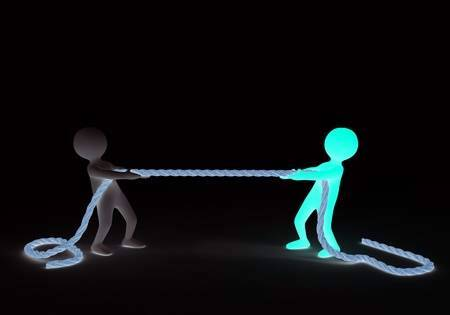
\includegraphics[scale=0.25]{figs/picture-tug-war2-neg.jpg} \\
  % \caption{}
  $p=\left(\frac{\alpha ^2 \log (1/\tau)}{4(\alpha +1) C\tau }\right)^{\alpha}$
\end{figure}
\end{frame}
% }}}
% {{{ 34.
\begin{frame}[label=current]
\begin{center}
  \renewcommand{\arraystretch}{1.8}
  \definecolor{LightCyan}{rgb}{0.88,1,1}
  \definecolor{Gray}{gray}{0.85}
  \scalebox{0.9}{
  \begin{tabular}{ |c| c| c |c| c| }
    \hline
                                                                 &   \thead{Mueller '91\\ Shiga '94}      &   \thead{L.C. \&\\ Kim '05}                                                            &   \thead{Tessitore \& \\ Zabczyk '98}  &   \thead{L.C. \& \\ Huang '19} \\ \hline\hline
    Eq.                                                          &   SHE on $\R$                          &   Frac. SHE on $\R$                                                                    &   \multicolumn{2}{>{\columncolor{darkpurple}}c|}{SHE on $\R^d$} \\ \hline
    Noise                                                        &   \multicolumn{2}{c|}{white in space}  &   \multicolumn{1}{c|}{\tabularCenterstack{c}{Colored; Strong \\ restrictions on $f$}}  &   \cellcolor{darkpurple} Dalang's Condition+ \\ \hline
    \multicolumn{1}{|c|}{\tabularCenterstack{c}{Init. \\ data}}  &   Functions                            &   Rough                                                                                &   Functions                            &   \cellcolor{darkpurple} Rough \\ \hline
  \end{tabular}
  }
\end{center}
\vfill
\vspace{3em}
\hfill \noindent\textcolor{gray}{\rule{0.5\textwidth}{0.6pt}}\\[0.3em]
\hfill \begin{minipage}{0.5\textwidth}
  \footnotesize\textcolor{gray}{
  $\dagger$ Dalang' conditions+: $\alpha\in(0,1]$,
  \[\int_{\R^d}\frac{\widehat{f}(\ud \xi)}{(1+|\xi|^2)^{1-\alpha}}<\infty. \tag{DL+}\]
  }
\end{minipage}
\end{frame}
% }}}
% {{{ 35. Ref.
\begin{frame}<10>
\footnotesize
{\bf\noindent Sample-path comparison principle:}
\begin{enumerate}
  \item \textcolor{yellow!75!black}{Mueller, C.} On the support of solutions to the heat equation with noise.                                                                                                             \textcolor{blue}{ \it Stochastics Stochastics Rep.              } 1991
  \item \textcolor{yellow!75!black}{Shiga, T.} Two contrasting properties of solutions for one-dimensional stochastic partial differential equations.                                                                     \textcolor{blue}{ \it Canad. J. Math.                           } 1994
  \item \textcolor{yellow!75!black}{Tessitore, G.} and \textcolor{yellow!75!black}{J. Zabczyk}. Strict positivity for stochastic heat equations.                                                                                   \textcolor{blue}{ \it Stochastic Process. Appl.                 } 1998
  \item[ \textcolor{magenta}{\bf 4.} ]\textcolor{yellow!75!black}{L.C.} and \textcolor{yellow!75!black}{K. Kim}. On comparison principle and strict positivity of solutions to the nonlinear stochastic fractional heat equations. \textcolor{blue}{ \it Ann. Inst. Henri Poincar\'e Probab. Stat. } 2017
  \item[ \textcolor{magenta}{\bf 5.} ] \textcolor{yellow!75!black}{L.C.} and \textcolor{yellow!75!black}{J. Huang.} Comparison principle for stochastic heat equation on $\R^d$.                                                   \textcolor{blue}{ \it Ann. Probab.                              } 2019
\end{enumerate}
\vfill
{\bf\noindent Stochastic (moment) comparison principle:}
\begin{enumerate}
  \item \textcolor{yellow!75!black}{Cox, J. T.}, \textcolor{yellow!75!black}{K. Fleischmann} and \textcolor{yellow!75!black}{A. Greven}. Comparison of interacting diffusions and an application to their ergodic theory.                  \textcolor{blue}{ \it Probab. Theory Related Fields           }1996
  \item \textcolor{yellow!75!black}{Tribe, R.} and \textcolor{yellow!75!black}{J. Zabczyk}. Notes on stochastic comparisons theorems for SDEs and SPDEs.                                                                          \textcolor{blue}{ \it Unpublished note, private communication }2013
  \item \textcolor{yellow!75!black}{Joseph, M.}, \textcolor{yellow!75!black}{D. Khoshnevisan} and \textcolor{yellow!75!black}{C. Mueller}. Strong invariance and noise-comparison principles for some parabolic stochastic PDEs.           \textcolor{blue}{ \it Ann. Probab.                            }2017
  \item \textcolor{yellow!75!black}{Foondun, M.}, \textcolor{yellow!75!black}{M. Joseph} and \textcolor{yellow!75!black}{S.T. Li}. An approximation result for a class of stochastic heat equations.                                       \textcolor{blue}{ \it Ann. Appl. Probab.                      }2018
  \item[\textcolor{magenta}{\bf 5.}] \textcolor{yellow!75!black}{L.C.} and \textcolor{yellow!75!black}{K. Kim.} Stochastic comparison principle for stochastic heat equation.                                                     \textcolor{blue}{ \it Electron. J. Probab.                    }2020
\end{enumerate}
\end{frame}
% }}}
% {{{ 36. Acknowledge
\begin{frame}<13>
\footnotesize
\hfill
\begin{minipage}{0.45\textwidth}
\begin{center}
  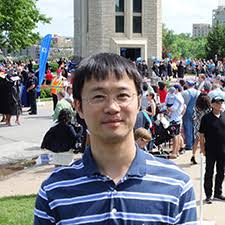
\includegraphics[scale=0.25]{figs/Jingyu.jpeg}\\
  Jingyu Huang\\
  University of Birmingham\\
  UK
\end{center}
\end{minipage}
\begin{minipage}{0.45\textwidth}
\begin{center}
  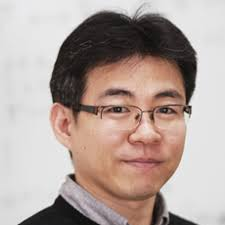
\includegraphics[scale=0.25]{figs/Kunwoo.jpeg}\\
  Kunwoo Kim\\
  Pohang University of Science and Technology, Korea
\end{center}
\end{minipage}
\vfill
\begin{enumerate}
  \item[-] \footnotesize L.C. and K. Kim: On comparison principle and strict positivity of solutions to the nonlinear stochastic fractional heat equations. \textcolor {blue}{\it  Ann. Inst. Henri Poincaré Probab. Stat.} 53 (2017), no. 1, 358--388.
  \item[-] \footnotesize L.C. and J. Huang: Comparison principle for stochastic heat equation on $\R^d$.                                                    \textcolor {blue}{\it Ann. Probab.}, 2019, Vol. 47, No. 2, 989--1035.
  \item[-] \footnotesize L.C. and K. Kim: Stochastic comparison for stochastic heat equation on $\R^d$.                                                     \textcolor {blue}{\it Electron. J. Probab.}, 2020.
  %   \pause
  %   \vfill
  % \item Raluca Balan\hfill University of Ottawa, CA
  % \item Michael Cranston \hfill University of California, Irvine
  % \item[Superv.] Robert Dalang \hfill \'{E}cole Polytechnique F\'{e}d\'{e}rale de Lausanne, CH
  % \item Guannan Hu \hfill University of Missouri-St. Louis
  % \item[Postd.] Yaozhong Hu \hfill University of Alberta, CA
  % \item Jingyu Huang \hfill University of Birmingham, UK
  % \item[Postd.] Davar Khoshnevisan \hfill University of Utah
  % \item Kunwoo Kim \hfill Pohang University of Science and Technology, KR
  % \item[Postd.] David Nualart \hfill University of Kansas
  % \item Fei Pu\hfill University of Utah
  \vfill
  \item[]\begin{center}
          {\Huge
          Thank you for listening!}\\[1em]
          {\small
 Le Chen (le.chen@emory.edu)}
         \end{center}
\pause
 \end{enumerate}
\end{frame}
% }}}
\end{document}


% {{{ Trotter's product formula
\begin{frame}<4>
 \begin{itemize}
  \item[] Let $T^{(\kappa,\rho)}_t$ denote the semigroup of the diffusion process with \\[1em]
     -- $\kappa$: drift parameter \\[0.5em]
     -- $\rho$: diffusion coefficient
  \bigskip
  \item \textcolor{yellow!75!black}{\bf Trotter's product formula} tells us that $\lim_{k\rightarrow\infty}\left[ T_{t/k}^{(\kappa,0)} T_{t/k}^{(0,\rho)}\right]^k=T_t^{(\kappa,\rho)}$.
  \vfill
  \item[] $\hspace{0em}\kappa=0:\hspace{2em}G^{(0,\rho)},T^{(0,\rho)}\hspace{2em}\begin{cases}
    \displaystyle dU(t, i)=\rho\left(U(t, i) \right) d M_i(t)\\
    \displaystyle U(0,i) = u_0(i)
    \end{cases}$
  \vfill
  \item[] $\hspace{3em}\rho\equiv0:\hspace{2em}G^{(\kappa,0)},T^{(\kappa,0)}\hspace{2em}\begin{cases}
    dU(t, i)=\kappa \sum_{j=1}^d (p_{i,j}-\delta_{i,j}) U(s,j) \ud t\\
    U(0,i) = u_0(i)
    \end{cases}$
 \end{itemize}
\end{frame}
% }}}
